\documentclass[12pt,]{book}
\usepackage{lmodern}
\usepackage{amssymb,amsmath}
\usepackage{ifxetex,ifluatex}
\usepackage{fixltx2e} % provides \textsubscript
\ifnum 0\ifxetex 1\fi\ifluatex 1\fi=0 % if pdftex
  \usepackage[T1]{fontenc}
  \usepackage[utf8]{inputenc}
\else % if luatex or xelatex
  \ifxetex
    \usepackage{mathspec}
  \else
    \usepackage{fontspec}
  \fi
  \defaultfontfeatures{Ligatures=TeX,Scale=MatchLowercase}
\fi
% use upquote if available, for straight quotes in verbatim environments
\IfFileExists{upquote.sty}{\usepackage{upquote}}{}
% use microtype if available
\IfFileExists{microtype.sty}{%
\usepackage{microtype}
\UseMicrotypeSet[protrusion]{basicmath} % disable protrusion for tt fonts
}{}
\usepackage[margin=1in]{geometry}
\usepackage{hyperref}
\hypersetup{unicode=true,
            pdftitle={Lecture Notes: Introduction to Data Science},
            pdfauthor={Héctor Corrada Bravo},
            pdfborder={0 0 0},
            breaklinks=true}
\urlstyle{same}  % don't use monospace font for urls
\usepackage{color}
\usepackage{fancyvrb}
\newcommand{\VerbBar}{|}
\newcommand{\VERB}{\Verb[commandchars=\\\{\}]}
\DefineVerbatimEnvironment{Highlighting}{Verbatim}{commandchars=\\\{\}}
% Add ',fontsize=\small' for more characters per line
\usepackage{framed}
\definecolor{shadecolor}{RGB}{248,248,248}
\newenvironment{Shaded}{\begin{snugshade}}{\end{snugshade}}
\newcommand{\KeywordTok}[1]{\textcolor[rgb]{0.13,0.29,0.53}{\textbf{#1}}}
\newcommand{\DataTypeTok}[1]{\textcolor[rgb]{0.13,0.29,0.53}{#1}}
\newcommand{\DecValTok}[1]{\textcolor[rgb]{0.00,0.00,0.81}{#1}}
\newcommand{\BaseNTok}[1]{\textcolor[rgb]{0.00,0.00,0.81}{#1}}
\newcommand{\FloatTok}[1]{\textcolor[rgb]{0.00,0.00,0.81}{#1}}
\newcommand{\ConstantTok}[1]{\textcolor[rgb]{0.00,0.00,0.00}{#1}}
\newcommand{\CharTok}[1]{\textcolor[rgb]{0.31,0.60,0.02}{#1}}
\newcommand{\SpecialCharTok}[1]{\textcolor[rgb]{0.00,0.00,0.00}{#1}}
\newcommand{\StringTok}[1]{\textcolor[rgb]{0.31,0.60,0.02}{#1}}
\newcommand{\VerbatimStringTok}[1]{\textcolor[rgb]{0.31,0.60,0.02}{#1}}
\newcommand{\SpecialStringTok}[1]{\textcolor[rgb]{0.31,0.60,0.02}{#1}}
\newcommand{\ImportTok}[1]{#1}
\newcommand{\CommentTok}[1]{\textcolor[rgb]{0.56,0.35,0.01}{\textit{#1}}}
\newcommand{\DocumentationTok}[1]{\textcolor[rgb]{0.56,0.35,0.01}{\textbf{\textit{#1}}}}
\newcommand{\AnnotationTok}[1]{\textcolor[rgb]{0.56,0.35,0.01}{\textbf{\textit{#1}}}}
\newcommand{\CommentVarTok}[1]{\textcolor[rgb]{0.56,0.35,0.01}{\textbf{\textit{#1}}}}
\newcommand{\OtherTok}[1]{\textcolor[rgb]{0.56,0.35,0.01}{#1}}
\newcommand{\FunctionTok}[1]{\textcolor[rgb]{0.00,0.00,0.00}{#1}}
\newcommand{\VariableTok}[1]{\textcolor[rgb]{0.00,0.00,0.00}{#1}}
\newcommand{\ControlFlowTok}[1]{\textcolor[rgb]{0.13,0.29,0.53}{\textbf{#1}}}
\newcommand{\OperatorTok}[1]{\textcolor[rgb]{0.81,0.36,0.00}{\textbf{#1}}}
\newcommand{\BuiltInTok}[1]{#1}
\newcommand{\ExtensionTok}[1]{#1}
\newcommand{\PreprocessorTok}[1]{\textcolor[rgb]{0.56,0.35,0.01}{\textit{#1}}}
\newcommand{\AttributeTok}[1]{\textcolor[rgb]{0.77,0.63,0.00}{#1}}
\newcommand{\RegionMarkerTok}[1]{#1}
\newcommand{\InformationTok}[1]{\textcolor[rgb]{0.56,0.35,0.01}{\textbf{\textit{#1}}}}
\newcommand{\WarningTok}[1]{\textcolor[rgb]{0.56,0.35,0.01}{\textbf{\textit{#1}}}}
\newcommand{\AlertTok}[1]{\textcolor[rgb]{0.94,0.16,0.16}{#1}}
\newcommand{\ErrorTok}[1]{\textcolor[rgb]{0.64,0.00,0.00}{\textbf{#1}}}
\newcommand{\NormalTok}[1]{#1}
\usepackage{longtable,booktabs}
\usepackage{graphicx,grffile}
\makeatletter
\def\maxwidth{\ifdim\Gin@nat@width>\linewidth\linewidth\else\Gin@nat@width\fi}
\def\maxheight{\ifdim\Gin@nat@height>\textheight\textheight\else\Gin@nat@height\fi}
\makeatother
% Scale images if necessary, so that they will not overflow the page
% margins by default, and it is still possible to overwrite the defaults
% using explicit options in \includegraphics[width, height, ...]{}
\setkeys{Gin}{width=\maxwidth,height=\maxheight,keepaspectratio}
\IfFileExists{parskip.sty}{%
\usepackage{parskip}
}{% else
\setlength{\parindent}{0pt}
\setlength{\parskip}{6pt plus 2pt minus 1pt}
}
\setlength{\emergencystretch}{3em}  % prevent overfull lines
\providecommand{\tightlist}{%
  \setlength{\itemsep}{0pt}\setlength{\parskip}{0pt}}
\setcounter{secnumdepth}{5}
% Redefines (sub)paragraphs to behave more like sections
\ifx\paragraph\undefined\else
\let\oldparagraph\paragraph
\renewcommand{\paragraph}[1]{\oldparagraph{#1}\mbox{}}
\fi
\ifx\subparagraph\undefined\else
\let\oldsubparagraph\subparagraph
\renewcommand{\subparagraph}[1]{\oldsubparagraph{#1}\mbox{}}
\fi

%%% Use protect on footnotes to avoid problems with footnotes in titles
\let\rmarkdownfootnote\footnote%
\def\footnote{\protect\rmarkdownfootnote}

%%% Change title format to be more compact
\usepackage{titling}

% Create subtitle command for use in maketitle
\newcommand{\subtitle}[1]{
  \posttitle{
    \begin{center}\large#1\end{center}
    }
}

\setlength{\droptitle}{-2em}
  \title{Lecture Notes: Introduction to Data Science}
  \pretitle{\vspace{\droptitle}\centering\huge}
  \posttitle{\par}
\subtitle{CSMC320, University of Maryland, College Park}
  \author{Héctor Corrada Bravo}
  \preauthor{\centering\large\emph}
  \postauthor{\par}
  \predate{\centering\large\emph}
  \postdate{\par}
  \date{2018-01-19}


\usepackage{amsthm}
\newtheorem{theorem}{Theorem}[chapter]
\newtheorem{lemma}{Lemma}[chapter]
\theoremstyle{definition}
\newtheorem{definition}{Definition}[chapter]
\newtheorem{corollary}{Corollary}[chapter]
\newtheorem{proposition}{Proposition}[chapter]
\theoremstyle{definition}
\newtheorem{example}{Example}[chapter]
\theoremstyle{definition}
\newtheorem{exercise}{Exercise}[chapter]
\theoremstyle{remark}
\newtheorem*{remark}{Remark}
\newtheorem*{solution}{Solution}
\begin{document}
\maketitle

{
\setcounter{tocdepth}{2}
\tableofcontents
}
\chapter{Preamble}\label{preamble}

These are lecture notes for \href{/}{CSMC320, Introduction to Data
Science} at the University of Maryland, College Park.

Refer to the \href{/}{Course Web Page} for further information.

\chapter{Introduction and Overview}\label{introduction-and-overview}

\section{What is Data Science?}\label{what-is-data-science}

Data science encapsulates the interdisciplinary activities required to
create data-centric artifacts and applications that address specific
scientific, socio-political, business, or other questions.

Let's look at the constiuent parts of this statement:

\subsection{Data}\label{data}

Measureable units of information gathered or captured from activity of
people, places and things.

\subsection{Specific Questions}\label{specific-questions}

Seeking to understand a phenomenon, natural, social or other, can we
formulate specific questions for which an answer posed in terms of
patterns observed, tested and or modeled in data is appropriate.

\subsection{Interdisciplinary
Activities}\label{interdisciplinary-activities}

Formulating a question, assessing the appropriateness of the data and
findings used to find an answer require understanding of the specific
subject area. Deciding on the appropriateness of models and inferences
made from models based on the data at hand requires understanding of
statistical and computational methods.

\subsection{Data-centric artifacts and
applications}\label{data-centric-artifacts-and-applications}

Answers to questions derived from data are usually shared and published
in meaningful, succint but sufficient, reproducible artifacts (papers,
books, movies, comics). Going a step further, interactive applications
that let others explore data, models and inferences are great.

\section{Why Data Science?}\label{why-data-science}

The granularity, size and accessibility data, comprising both physical,
social, commercial and political spheres has exploded in the last decade
or more.

\begin{quote}
I keep saying that the sexy job in the next 10 years will be
statisticians''
\end{quote}

\begin{quote}
Hal Varian, Chief Economist at Google
(\url{http://www.nytimes.com/2009/08/06/technology/06stats.html?_r=0})
\end{quote}

\begin{quote}
``The ability to take data---to be able to understand it, to process it,
to extract value from it, to visualize it, to communicate it---that's
going to be a hugely important skill in the next decades, not only at
the professional level but even at the educational level for elementary
school kids, for high school kids, for college kids.''
\end{quote}

\begin{quote}
``Because now we really do have essentially free and ubiquitous data. So
the complimentary scarce factor is the ability to understand that data
and extract value from it.''
\end{quote}

\begin{quote}
Hal Varian
(\url{http://www.mckinsey.com/insights/innovation/hal_varian_on_how_the_web_challenges_managers})
\end{quote}

\section{Data Science in Humanities and Social
Sciences}\label{data-science-in-humanities-and-social-sciences}

Because of the large amount of data produced across many spheres of
human social and creative activity, many questions in the humanities and
social sciences may be addressed by establishing patterns in data. In
the humanities, this can range from unproblematic quesitions of how to
dissect a large creative corpora, say music, literature, based on raw
characteristics of those works, text, sound and image. To more
problematic questions, of analysis of intent, understanding,
appreciation and valuation of these creative corpora.

In the social sciences, issues of fairness and transparency in the
current era of big data are especially problematic. Is data collected
representative of population for which inferences are drawn? Are methods
employed learning latent unfair factors from ostensibly fair data? These
are issues that the research community is now starting to address.

In all settings, issues of ethical collection of data, application of
models, and deployment of data-centric artifacts are essential to
grapple with. Issues of privacy are equally important.

\section{Course organization}\label{course-organization}

This course will cover basics of how to use the R data analysis
environment for data science activities in humanities and social
science. The general organization of the course will be the following:

\subsection{Day 1: Introduction and
preparation}\label{day-1-introduction-and-preparation}

\begin{itemize}
\tightlist
\item
  Get ourselved settled with R
\item
  Formulating a question that can be addressed with data
\item
  How to get data to address a specific question
\item
  How to manipulate this data to get to what we need for our question of
  interest
\item
  How to visualize this data
\end{itemize}

\subsection{Day 2: Use cases}\label{day-2-use-cases}

\begin{itemize}
\tightlist
\item
  Social media analysis: text and network structures
\item
  Fitting and evaluating regression models in R
\item
  Text analysis
\item
  Machine Learning modeling in R
\item
  Survey analysis
\item
  Nested models in R
\end{itemize}

\subsection{Day 3: Presentation and
teaching}\label{day-3-presentation-and-teaching}

\begin{itemize}
\tightlist
\item
  How to present and publish analysis using R
\item
  Using R in teaching
\end{itemize}

\section{General Workflow}\label{general-workflow}

The data science activities we will cover are roughly organized into a
general workflow that will help us navigate this material.

\begin{figure}
\centering
\includegraphics{img/zumel_mount_cycle.png}
\caption{}
\end{figure}

\subsection{Defining the goal}\label{defining-the-goal}

\begin{itemize}
\tightlist
\item
  What is the question/problem?
\item
  Who wants to answer/solve it?
\item
  What do they know/do now?
\item
  How well can we expect to answer/solve it?
\item
  How well do they want us to answer/solve it?
\end{itemize}

\subsection{Data collection and
Management}\label{data-collection-and-management}

\begin{itemize}
\tightlist
\item
  What data is available?
\item
  Is it good enough?
\item
  Is it enough?
\item
  What are sensible measurements to derive from this data? Units,
  transformations, rates, ratios, etc.
\end{itemize}

\subsection{Modeling}\label{modeling}

\begin{itemize}
\tightlist
\item
  What kind of problem is it? E.g., classification, clustering,
  regression, etc.
\item
  What kind of model should I use?
\item
  Do I have enough data for it?
\item
  Does it really answer the question?
\end{itemize}

\subsection{Model evaluation}\label{model-evaluation}

\begin{itemize}
\tightlist
\item
  Did it work? How well?
\item
  Can I interpret the model?
\item
  What have I learned?
\end{itemize}

\subsection{Presentation}\label{presentation}

\begin{itemize}
\tightlist
\item
  Again, what are the measurements that tell the real story?
\item
  How can I describe and visualize them effectively?
\end{itemize}

\subsection{Deployment}\label{deployment}

\begin{itemize}
\tightlist
\item
  Where will it be hosted?
\item
  Who will use it?
\item
  Who will maintain it?
\end{itemize}

\chapter{An Illustrative Analysis}\label{an-illustrative-analysis}

\url{http://fivethirtyeight.com} has a clever series of articles on the
types of movies different actors make in their careers:
\url{https://fivethirtyeight.com/tag/hollywood-taxonomy/}

I'd like to do a similar analysis. Let's do this in order:

\begin{enumerate}
\def\labelenumi{\arabic{enumi})}
\tightlist
\item
  Let's do this analysis for Diego Luna
\item
  Let's use a clustering algorithm to determine the different types of
  movies they make
\item
  Then, let's write an application that performs this analysis for any
  actor and test it with Gael García Bernal
\item
  Let's make the application interactive so that a user can change the
  actor and the number of movie clusters the method learns.
\end{enumerate}

For now, we will go step by step through this analysis without showing
how we perform this analysis using R. As the course progresses, we will
learn how to carry out these steps.

\section{Gathering data}\label{gathering-data}

\subsection{Movie ratings}\label{movie-ratings}

For this analysis we need to get the movies Diego Luna was in, along
with their Rotten Tomatoes ratings. For that we scrape this webpage:
\url{https://www.rottentomatoes.com/celebrity/diego_luna}.

Once we scrape the data from the Rotten Tomatoes website and clean it
up, this is part of what we have so far:

\begin{tabular}{r|l|l|l|r}
\hline
RATING & TITLE & CREDIT & BOX OFFICE & YEAR\\
\hline
85 & Rogue One: A Star Wars Story & Captain Cassian Andor & \$532.2M & 2016\\
\hline
89 & Blood Father & Jonah & — & 2016\\
\hline
82 & The Book of Life & Manolo & — & 2014\\
\hline
100 & I Stay with You (Me quedo contigo) & Actor & — & 2014\\
\hline
67 & Elysium & Julio & \$90.8M & 2013\\
\hline
41 & Casa de mi padre & Raul & \$5.9M & 2012\\
\hline
51 & Contraband & Gonzalo & \$66.5M & 2012\\
\hline
\end{tabular}

This data includes, for each of the movies Diego Luna has acted in, the
rotten tomatoes rating, the movie title, Diego Luna's role in the movie,
the U.S. domestic gross and the year of release.

\subsection{Movie budgets and revenue}\label{movie-budgets-and-revenue}

For the movie budgets and revenue data we scrape this webpage:
\url{http://www.the-numbers.com/movie/budgets/all}

This is part of what we have for that table after scraping and cleaning
up:

\begin{tabular}{l|l|r|r|r}
\hline
release\_date & movie & production\_budget & domestic\_gross & worldwide\_gross\\
\hline
2009-12-18 & Avatar & 425 & 760.50762 & 2783.9190\\
\hline
2015-12-18 & Star Wars Ep. VII: The Force Awakens & 306 & 936.66223 & 2058.6622\\
\hline
2007-05-24 & Pirates of the Caribbean: At World’s End & 300 & 309.42043 & 963.4204\\
\hline
2015-11-06 & Spectre & 300 & 200.07417 & 879.6209\\
\hline
2012-07-20 & The Dark Knight Rises & 275 & 448.13910 & 1084.4391\\
\hline
2013-07-02 & The Lone Ranger & 275 & 89.30212 & 260.0021\\
\hline
2012-03-09 & John Carter & 275 & 73.05868 & 282.7781\\
\hline
2010-11-24 & Tangled & 260 & 200.82194 & 586.5819\\
\hline
2017-06-21 & Transformers: The Last Knight & 260 & 0.00000 & 0.0000\\
\hline
2007-05-04 & Spider-Man 3 & 258 & 336.53030 & 890.8753\\
\hline
\end{tabular}

This data is for 5368 movies, including its release date, title,
production budget, US domestic and worlwide gross earnings. The latter
three are in millions of U.S. dollars.

One thing we might want to check is if the budget and gross entries in
this table are inflation adjusted or not. To do this, we can make a plot
of domestic gross, which we are using for the subsequent analyses.

\begin{verbatim}
## Loading required package: methods
\end{verbatim}

\begin{verbatim}
## 
## Attaching package: 'lubridate'
\end{verbatim}

\begin{verbatim}
## The following object is masked from 'package:base':
## 
##     date
\end{verbatim}

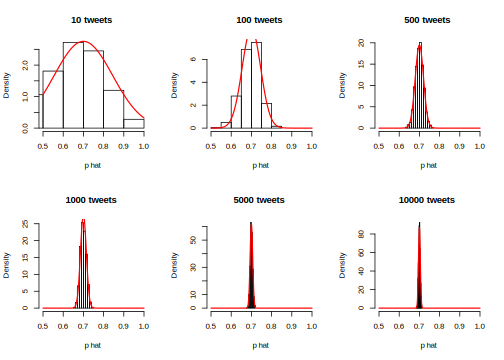
\includegraphics{mtec_cadi_2017_files/figure-latex/unnamed-chunk-5-1.pdf}

Although we don't know for sure, since the source of our data does not
state this specifically, it looks like the domestic gross measurement is
inflation adjusted since average gross is stable across years.

\section{Manipulating the data}\label{manipulating-the-data}

Next, we combine the datasets we obtained to get closer to the data we
need to make the plot we want.

We combine the two datasets using the movie title, so that the end
result has the information in both tables for each movie.

\begin{tabular}{r|l|l|l|r|l|r|r|r}
\hline
RATING & TITLE & CREDIT & BOX OFFICE & YEAR & release\_date & production\_budget & domestic\_gross & worldwide\_gross\\
\hline
85 & Rogue One: A Star Wars Story & Captain Cassian Andor & \$532.2M & 2016 & 2016-12-16 & 200.0 & 532.17732 & 1050.98849\\
\hline
82 & The Book of Life & Manolo & — & 2014 & 2014-10-17 & 50.0 & 50.15154 & 97.65154\\
\hline
67 & Elysium & Julio & \$90.8M & 2013 & 2013-08-09 & 120.0 & 93.05012 & 286.19209\\
\hline
51 & Contraband & Gonzalo & \$66.5M & 2012 & 2012-01-13 & 25.0 & 66.52800 & 98.40685\\
\hline
94 & Milk & Jack Lira & \$31.8M & 2008 & 2008-11-26 & 20.0 & 31.84130 & 57.29337\\
\hline
69 & Criminal & Rodrigo & \$0.8M & 2004 & 2016-04-15 & 31.5 & 14.70870 & 38.77126\\
\hline
61 & The Terminal & Enrique Cruz & \$77.1M & 2004 & 2004-06-18 & 75.0 & 77.07396 & 218.67396\\
\hline
79 & Open Range & Button & \$58.3M & 2003 & 2003-08-15 & 26.0 & 58.33125 & 68.61399\\
\hline
76 & Frida & Alejandro Gomez & \$25.7M & 2002 & 2002-10-25 & 12.0 & 25.88500 & 56.13124\\
\hline
\end{tabular}

\section{Visualizing the data}\label{visualizing-the-data}

Now that we have the data we need, we can make a plot:

\begin{figure}
\centering
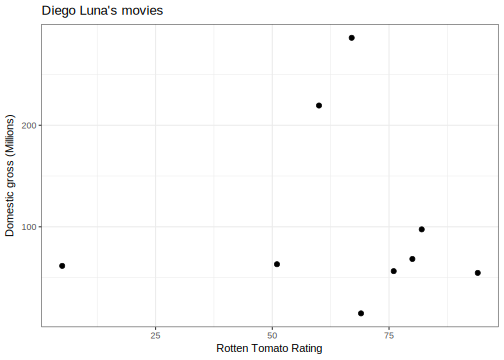
\includegraphics{mtec_cadi_2017_files/figure-latex/unnamed-chunk-8-1.pdf}
\caption{\label{fig:unnamed-chunk-8}Ratings and U.S. Domestic Gross of Diego
Luna's movies.}
\end{figure}

We see that there is one clear outlier in Diego Luna's movies, which
probably is the one Star Wars movie he acted in. The remaining movies
could potentially be grouped into two types of movies, those with higher
rating and those with lower ratings.

\section{Modeling data}\label{modeling-data}

We can use a clustering algorithm to partition Diego Luna's movies. We
can use the data we obtained so far and see if the k-means clustering
algorithm partitions these movies into three sensible groups using the
movie's rating and domestic gross.

Let's see how the movies are grouped:

\begin{tabular}{l|r|r|l}
\hline
TITLE & RATING & domestic\_gross & cluster\\
\hline
The Book of Life & 82 & 50.15154 & 1\\
\hline
Milk & 94 & 31.84130 & 1\\
\hline
Criminal & 69 & 14.70870 & 1\\
\hline
Frida & 76 & 25.88500 & 1\\
\hline
Rogue One: A Star Wars Story & 85 & 532.17732 & 2\\
\hline
Elysium & 67 & 93.05012 & 3\\
\hline
Contraband & 51 & 66.52800 & 3\\
\hline
The Terminal & 61 & 77.07396 & 3\\
\hline
Open Range & 79 & 58.33125 & 3\\
\hline
\end{tabular}

\section{Visualizing model result}\label{visualizing-model-result}

Let's remake the same plot as before, but use color to indicate each
movie's cluster assignment given by the k-means algorithm.

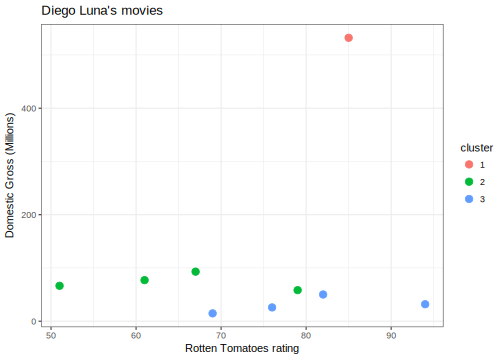
\includegraphics{mtec_cadi_2017_files/figure-latex/unnamed-chunk-11-1.pdf}

The algorithm did make the Star Wars movie it's own group since it's so
different that the other movies. The grouping of the remaining movies is
not as clean.

To make the plot and clustering more interpretable, let's annotate the
graph with some movie titles. In the k-means algorithm, each group of
movies is represented by an average rating and an average domestic
gross. What we can do is find the movie in each group that is closest to
the average and use that movie title to annotate each group in the plot.

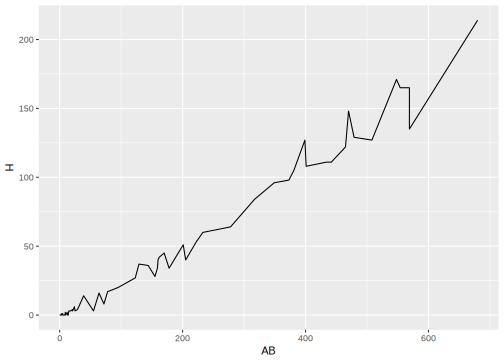
\includegraphics{mtec_cadi_2017_files/figure-latex/unnamed-chunk-13-1.pdf}

Roughly, movies are clustered into Star Wars and low vs.~high rated
movies. The latter seem to have some difference in domestic gross. For
example, movies like
\href{https://www.rottentomatoes.com/m/1133499_1133499_terminal}{``The
Terminal''} have lower rating but make slightly more money than movies
like \href{https://www.rottentomatoes.com/m/frida}{``Frida''}. We could
use statistical modeling to see if that's the case, but will skip that
for now. Do note also, that the clustering algorithm we used seems to be
assigning one of the movies incorrectly, which warrants further
investigation.

\section{Abstracting the analysis}\label{abstracting-the-analysis}

While not a tremendous success, we decide we want to carry on with this
analysis. We would like to do this for other actors' movies. One of the
big advantages of using R is that we can write a piece of code that
takes an actor's name as input, and reproduces the steps of this
analysis for that actor. We call these functions, we'll see them and use
them a lot in this course.

For our analysis, this function must do the following:

\begin{enumerate}
\def\labelenumi{\arabic{enumi}.}
\tightlist
\item
  Scrape movie ratings from Rotten Tomatoes
\item
  Clean up the scraped data
\item
  Join with the budget data we downloaded previously
\item
  Perform the clustering algorithm
\item
  Make the final plot
\end{enumerate}

With this in mind, we can write functions for each of these steps, and
then make one final function that puts all of these together.

For instance, let's write the scraping function. It will take an actor's
name and output the scraped data.

Let's test it with Gael García Bernal:

\begin{tabular}{l|l|l|l|r}
\hline
RATING & TITLE & CREDIT & BOX OFFICE & YEAR\\
\hline
No Score Yet & Viva - A vida é uma festa & Hector & — & 2017\\
\hline
97\% & Coco & Hector & \$192M & 2017\\
\hline
31\% & Salt and Fire & Dr. Fabio Cavani & — & 2017\\
\hline
\end{tabular}

Good start. We can then write functions for each of the steps we did
with Diego Luna before.

Then put all of these steps into one function that calls our new
functions to put all of our analysis together:

We can test this with Gael García Bernal

\begin{Shaded}
\begin{Highlighting}[]
\KeywordTok{analyze_actor}\NormalTok{(}\StringTok{"Gael Garcia Bernal"}\NormalTok{)}
\end{Highlighting}
\end{Shaded}

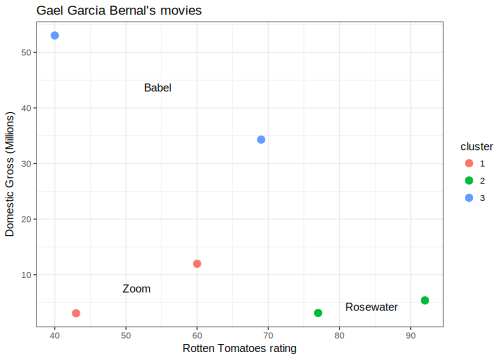
\includegraphics{mtec_cadi_2017_files/figure-latex/test_bbg-1.pdf}

\section{Making analyses accessible}\label{making-analyses-accessible}

Now that we have written a function to analyze an actor's movies, we can
make these analyses easier to produce by creating an interactive
application that wraps our new function. The \texttt{shiny} R package
makes creating this type of application easy.

\begin{center}\href{https://hcorrada.shinyapps.io/movie_app/}{\includegraphics{mtec_cadi_2017_files/figure-latex/movie_app-1} }\end{center}

\section{Summary}\label{summary}

In this analysis we saw examples of the common steps and operations in a
data analysis:

\begin{enumerate}
\def\labelenumi{\arabic{enumi})}
\item
  Data ingestion: we scraped and cleaned data from publicly accessible
  sites
\item
  Data manipulation: we integrated data from multiple sources to prepare
  our analysis
\item
  Data visualization: we made plots to explore patterns in our data
\item
  Data modeling: we made a model to capture the grouping patterns in
  data automatically, using visualization to explore the results of this
  modeling
\item
  Publishing: we abstracted our analysis into an application that allows
  us and others to perform this analysis over more datasets and explore
  the result of modeling using a variety of parameters
\end{enumerate}

\chapter{Setting up R}\label{setting-up-r}

Here we setup R, RStudio and anything else we will use in the course.

\section{Setting up R}\label{setting-up-r-1}

R is a free, open source, environment for data analysis. It is available
as a free binary download for Mac, Linux and Windows. For the more
adventorous, it can also be compiled from source. To install R in your
computer go to \url{https://cran.r-project.org/index.html} and download
and install the appropriate binary file.

\begin{figure}
\centering
\includegraphics{img/cran.png}
\caption{}
\end{figure}

This will install the base R system: the R programming language, a few
packages for common data analyses and a development environment.

\section{Setting up Rstudio}\label{setting-up-rstudio}

We will actually use Rstudio to interact with R. Rstudio is a very
powerful application to make data analysis with R easier to do. To
install go to \url{https://www.rstudio.com/products/rstudio/download/}
and download the appropriate version of Rstudio.

\begin{figure}
\centering
\includegraphics{img/rstudio.png}
\caption{}
\end{figure}

\section{A first look at Rstudio}\label{a-first-look-at-rstudio}

Let's take a first look at Rstudio. The first thing you will notice is
that Rstudio is divided into panes. Let's take a look first at the
\emph{Console}.

\subsection{Interactive Console}\label{interactive-console}

The most immediate way to interact with R is through the interactive
console. Here we can write R instructions to perform our data analyses.
We want to start using data so the first instructions we will look at
deal with loading data.

When you installed R, a few illustrative datasets were installed as
well. Let's take a look at the list of datasets you now have access to.
Write the following command in the console

\begin{figure}
\centering
\includegraphics{img/rstudio_data.png}
\caption{}
\end{figure}

This will list names and descriptions of datasets available in your R
installation. Let's try to find out more information about these
datasets. In R, the first attempt to get help with something is to use
the \texttt{?} operation. So, to get help about the \texttt{swiss}
dataset we can enter the following in the console

This will make the documentation for the \texttt{swiss} dataset open in
another pane.

\begin{figure}
\centering
\includegraphics{img/rstudio_swiss.png}
\caption{}
\end{figure}

\textbf{On your own:} Find more information about a different dataset
using the \texttt{?} operator.

\subsection{Data Viewer}\label{data-viewer}

According to the documentation we just saw for \texttt{swiss}, this is a
\texttt{data.frame} with 47 observations and 6 variables. The
\texttt{data.frame} is the basic structure we will use to represent data
throughout the course. We will see this again repeatedly, and use a
couple of other names (e.g., \texttt{tibble}) to refer to this.
Intuitively, you can think of the \texttt{data.frame} like a
spreadsheet, with rows representing observations, and columns
representing variables that describe those observations. Let's see what
the \texttt{swiss} data looks like using the Rstudio data viewer.

\begin{figure}
\centering
\includegraphics{img/rstudio_view_swiss.png}
\caption{}
\end{figure}

The Data Viewer lets you reorder data by the values in a column. It also
lets you filter rows of the data by values as well.

\textbf{On your own}: Use the Data Viewer to explore another of the
datasets you saw listed before.

\subsection{Names, values and
functions}\label{names-values-and-functions}

Let's make a very short pause to talk about something you may have
noticed. In the console, we've now written a few instructions, e.g.
\texttt{View(swiss)}. Let's take a closer look at how these instructions
are put together.

\emph{expressions}: first of all, we call these instructions
\emph{expressions}, which are just text that R can evaluate into a
value. \texttt{View(swiss)} is an expression.

\emph{values}: so, what's a value? They are numbers, strings, data
frames, etc. This is the data we will be working with. The number
\texttt{2} is a value. So is the string \texttt{"Hector"}.

So, what value is produced when R evaluates the expression
\texttt{View(swiss)}? Nothing, which we also treat as a value. That
wasn't very interesting, but it does have a side effect: it shows the
\texttt{swiss} dataset in the Data viewer.

How about a simpler expression: \texttt{swiss}, what value is produced
when R evaluates the expression \texttt{swiss}? The data.frame
containing that data. Try it out in the console.

\emph{names}: so if \texttt{swiss} isn't a value, what is it? It is a
\emph{name}. We use these to refer to values. So, when we write the
expression \texttt{swiss}, we tell R we want the \emph{value} referenced
by the name \texttt{swiss}, that is, the data itself!

\begin{figure}
\centering
\includegraphics{img/names_values.png}
\caption{}
\end{figure}

\emph{functions}: Besides numbers, strings, data frames, etc. another
important type of value is the \emph{function}. Functions are a series
of instructions that take some input value and produce a different
value. The name \texttt{View} refers to the function that takes a data
frame as input, and displays it in the Data viewer. Functions are called
using the parentheses we saw before: \texttt{View(swiss)}, the
parentheses say that you are passing input \texttt{swiss} to the
function \texttt{View}. We'll see later how we can write our own
functions.

\subsection{Plotting}\label{plotting}

Next, I want to show the \emph{Plots} pane in Rstudio. Let's make a plot
using the \texttt{swiss} dataset:

\begin{figure}
\centering
\includegraphics{img/rstudio_plot_swiss.png}
\caption{}
\end{figure}

It's not pretty, but it was very easy to produce. There's a couple of
things going on here\ldots{}

\begin{itemize}
\item
  \texttt{plot} is a function, it takes two inputs, the data to put in
  the x and y axes, evaluates to nothing, but creates a plot of the data
\item
  \texttt{swiss\$Education} is how we refer to the \texttt{Education}
  column in the \texttt{swiss} data frame.
\end{itemize}

\textbf{On your own}: Make a plot using other variables in the
\texttt{swiss} dataset.

\subsection{Editor}\label{editor}

So far, we've made some good progress: we know how to write expressions
on the R console so that they are evaluated, we are starting to get a
basic understanding of how these expressions are constructed, we can use
the Data viewer to explore data frames, and made one plot that was
displayed in the Plots pane. To finish this quick tour, I want to look
at two more Rstudio panes: the file editor, and the File viewer.

As you have noticed, everytime we want to evaluate an expression on the
console, we have to write it in. For example, if we want to change the
plot we made above to include a different variable, we have to write the
whole thing again. Also, what if I forgot what expression I used to make
a specific plot? Even better, what if I wanted somebody else to make the
plot I just made?

By far, one of the biggest advantages of using R over Excel or other
similar programs, is that we can write expressions in scripts that are
easy to share with others, making analyses easier to reproduce. Let's
write a script that we can use to make the same plot we just made.

In the Rstudio menu select
\texttt{File\textgreater{}New\ File\textgreater{}R\ Script}

\begin{figure}
\centering
\includegraphics{img/rstudio_new_script.png}
\caption{}
\end{figure}

This will open a tab in the File editor in which we can write
expressions:

\begin{figure}
\centering
\includegraphics{img/rstudio_file.png}
\caption{}
\end{figure}

We can then evaluate the expressions in the file one at a time, or all
at the same time.

We can then save these expressions in a script. In the Rstudio menu
select \texttt{File\textgreater{}Save} and save as a text file. The
convention is to use the \texttt{.R} or \texttt{.r} file extension,
e.g., \texttt{swiss\_plot.r}.

\textbf{On your own:} Add expressions for additional plots to the script
and save again. Run the new expressions.

\subsection{Files viewer}\label{files-viewer}

Rstudio includes a Files viewer that you can use to find and load files.
You can find the Files near the Plots viewer

\begin{figure}
\centering
\includegraphics{img/rstudio_files.png}
\caption{}
\end{figure}

\section{R packages}\label{r-packages}

Another of R's advantages for data analysis is that it has attracted a
large number of extremely useful additions provided by users worldwide.
These are housed in
\href{https://cran.r-project.org/web/packages/index.html}{CRAN}.

In this course we will make a lot of use of a set of packages bundled
together into the \texttt{tidyverse} by Hadley Wickham and others. These
packages make preparing, modeling and visualizing certain kinds data
(which covers the vast majority of use cases) quite fun and pleasent.
There is a webpage for the general tidyverse project:
\url{http://tidyverse.org}, which includes pages for each of the
packages included there.

Let's install the \texttt{tidyverse} into your R environment. There are
two ways of installing packages. In the console, you can use the
expression:

In Rstudio, you can use the \emph{Packages} tab:

\begin{figure}
\centering
\includegraphics{img/rstudio_install_packages.png}
\caption{}
\end{figure}

\textbf{On your own:} Install the following additional packages which we
will use later on: \texttt{rvest}, \texttt{stringr},
\texttt{nycflights13} and \texttt{broom}.

\section{Finishing your setup}\label{finishing-your-setup}

Go to the Google form as instructed and complete your exit ticket.

\chapter{R Principles}\label{r-principles}

Now that we have our tools ready, let's start doing some analysis.
First, let's go over some principles of R as a data analysis
environment. R is a computational environment for data analysis. It is
designed around a \emph{functional} language, as opposed to
\emph{procedural} languages like Java or C, that has desirable
properties for the type of operations and workflows that are frequently
performed in the course of analyzing datasets. In this exercise we will
start learning some of those desirable properties while performing an
analysis of a real dataset.

\section{Some history}\label{some-history}

R is an offspring of S, a language created in AT\&T Labs by John
Chambers (now at Stanford) and others in 1976 with the goal of creating
an environment for statistical computing and data analysis. The standard
for the language in current use was settled in 1998. That same year,
``S'' won the ACM Software System award, awarded to software systems
``that have a lasting influence, reflected in contributions to concepts,
in commercial acceptance, or both''.

In 1991, Robert Gentleman and Ross Ihaka created R to provide an open
source implementation of the S language and environment. They also
redesigned the language to enforce lexical scoping rules. It has been
maintained by the R core group since 1997, and in 2015 an R consortium,
including Microsoft, Google, and others, was created.

Along with Python it is one of the most popular environments for data
analysis (e.g., figure below from
\href{http://www.kdnuggets.com/2016/06/r-python-top-analytics-data-mining-data-science-software.html}{KDNuggets
2016 software survey})

\begin{figure}
\centering
\includegraphics{img/kdnuggets-2016.jpg}
\caption{}
\end{figure}

We use it for this class because we find that besides it being a
state-of-the-art data analysis environment, it provides a clean
end-to-end platform for teaching material across the data
management-modeling-communication spectrum that we study in class.

\section{Additional R resources}\label{additional-r-resources}

Resources for learning and reading about R are listed in our
\href{http://www.hcbravo.org/IntroDataScience/resources/}{here}. Of note
are the \href{http://swirlstats.com/}{swirl project} and DataCamp's
{[}introduction to R{]} course.

One of the biggest strengths of the R ecosystem is the variety and
quality of packages for data analysis available. R uses a package system
(like Python and Ruby for instance). Packages are divided into two
classes: \textbf{base} which are packages installed when R is installed,
includes packages for basic statistics, computing with probability
distributions, plotting and graphics, matrix manipulations and other),
all other packages are available in
\href{http://cran.r-project.org}{CRAN}. We will be using a fair number
of these packages through the course of the semester.

\section{Literate Programming}\label{literate-programming}

One last note before we get started. R has great support for
\href{http://en.wikipedia.org/wiki/Literate_programming}{literate
programming}, where source code that contains both code, the result of
evaluating that code, and text explaining that code co-exist in a single
document. This is extremely valuable in data analysis, as many choices
made by data analysts are worth explaning in text, and interpretation of
the results of analyses can co-exist with the computations used in that
analysis. This document you are reading contains both text and code. In
class, we will use \href{http://rmarkdown.rstudio.com/}{Rmarkdown} for
this purpose.

\section{A data analysis to get us
going}\label{a-data-analysis-to-get-us-going}

I'm going to do a very simple analysis of Baltimore crime to show off R.
We'll use data downloaded from Baltimore City's awesome open data site
(this was downloaded a couple of years ago so if you download now, you
will get different results).

The repository for this particular data is here.
\url{https://data.baltimorecity.gov/Crime/BPD-Arrests/3i3v-ibrt}

\section{Getting data}\label{getting-data}

We've prepared the data previously into a comma-separated value file
(\texttt{.csv} file). In this format, each line contains
\emph{attribute} values (separated by commas) for one \emph{entity} in
our dataset. Which we can download and load into our R environment.

The \texttt{read\_csv} command is part of the \texttt{readr} R package
and allows you to read a dataset stored in a csv file. This function is
extremely versatile, and you can read more about it by using the
standard help system in R: \texttt{?read\_csv}. Now, the result of
running calling this function is the data itself, so, by running the
function in the console, the result of the function is printed.

\section{Variables and Value}\label{variables-and-value}

To make use of this dataset we want to assign the result of calling
\texttt{read.csv} (i.e., the dataset) to a variable:

\begin{Shaded}
\begin{Highlighting}[]
\KeywordTok{library}\NormalTok{(tidyverse)}
\NormalTok{arrest_tab <-}\StringTok{ }\KeywordTok{read_csv}\NormalTok{(}\StringTok{"data/BPD_Arrests.csv"}\NormalTok{)}
\end{Highlighting}
\end{Shaded}

\begin{verbatim}
## Parsed with column specification:
## cols(
##   arrest = col_integer(),
##   age = col_integer(),
##   sex = col_character(),
##   race = col_character(),
##   arrestDate = col_character(),
##   arrestTime = col_time(format = ""),
##   arrestLocation = col_character(),
##   incidentOffense = col_character(),
##   incidentLocation = col_character(),
##   charge = col_character(),
##   chargeDescription = col_character(),
##   district = col_character(),
##   post = col_integer(),
##   neighborhood = col_character(),
##   `Location 1` = col_character()
## )
\end{verbatim}

Now we can ask what \emph{type} of value is stored in the
\texttt{arrest\_tab} variable:

\begin{Shaded}
\begin{Highlighting}[]
\KeywordTok{class}\NormalTok{(arrest_tab)}
\end{Highlighting}
\end{Shaded}

\begin{verbatim}
## [1] "tbl_df"     "tbl"        "data.frame"
\end{verbatim}

The \texttt{data.frame} is a workhorse data structure in R. It
encapsulates the idea of \emph{entities} (in rows) and \emph{attribute
values} (in columns). We can ask other features of this dataset:

\begin{Shaded}
\begin{Highlighting}[]
\CommentTok{# This is a comment in R, by the way}

\CommentTok{# How many rows (entities) does this dataset contain?}
\KeywordTok{nrow}\NormalTok{(arrest_tab)}
\end{Highlighting}
\end{Shaded}

\begin{verbatim}
## [1] 104528
\end{verbatim}

\begin{Shaded}
\begin{Highlighting}[]
\CommentTok{# How many columns (attributes)?}
\KeywordTok{ncol}\NormalTok{(arrest_tab)}
\end{Highlighting}
\end{Shaded}

\begin{verbatim}
## [1] 15
\end{verbatim}

\begin{Shaded}
\begin{Highlighting}[]
\CommentTok{# What are the names of those columns?}
\KeywordTok{colnames}\NormalTok{(arrest_tab)}
\end{Highlighting}
\end{Shaded}

\begin{verbatim}
##  [1] "arrest"            "age"               "sex"              
##  [4] "race"              "arrestDate"        "arrestTime"       
##  [7] "arrestLocation"    "incidentOffense"   "incidentLocation" 
## [10] "charge"            "chargeDescription" "district"         
## [13] "post"              "neighborhood"      "Location 1"
\end{verbatim}

Now, in Rstudio you can view the data frame using
\texttt{View(arrest\_tab)}.

\section{Indexing}\label{indexing}

A basic operation in data analysis is selecting subsets of a dataset.
For that we can use a few alternative options for \emph{indexing} into
datasets.

\begin{Shaded}
\begin{Highlighting}[]
\CommentTok{# to obtain the value in the first row, fifth column:}
\NormalTok{arrest_tab[}\DecValTok{1}\NormalTok{,}\DecValTok{5}\NormalTok{]}
\end{Highlighting}
\end{Shaded}

\begin{verbatim}
## # A tibble: 1 x 1
##   arrestDate
##   <chr>     
## 1 01/01/2011
\end{verbatim}

\begin{Shaded}
\begin{Highlighting}[]
\CommentTok{# note that indexing in R is 1-based, not 0-based, so the first row is indexed by 1}

\CommentTok{# now we want to do a bit more, so let's say we want the value in the fifth column of our dataset for the first 10 rows. For that we can use slice notation:}
\NormalTok{arrest_tab[}\DecValTok{1}\OperatorTok{:}\DecValTok{10}\NormalTok{,}\DecValTok{5}\NormalTok{]}
\end{Highlighting}
\end{Shaded}

\begin{verbatim}
## # A tibble: 10 x 1
##    arrestDate
##    <chr>     
##  1 01/01/2011
##  2 01/01/2011
##  3 01/01/2011
##  4 01/01/2011
##  5 01/01/2011
##  6 01/01/2011
##  7 01/01/2011
##  8 01/01/2011
##  9 01/01/2011
## 10 01/01/2011
\end{verbatim}

\begin{Shaded}
\begin{Highlighting}[]
\CommentTok{# similarly, to obtain the value in the first five columns of the first row}
\NormalTok{arrest_tab[}\DecValTok{1}\NormalTok{,}\DecValTok{1}\OperatorTok{:}\DecValTok{5}\NormalTok{]}
\end{Highlighting}
\end{Shaded}

\begin{verbatim}
## # A tibble: 1 x 5
##     arrest   age sex   race  arrestDate
##      <int> <int> <fct> <fct> <chr>     
## 1 11126858    23 B     M     01/01/2011
\end{verbatim}

\begin{Shaded}
\begin{Highlighting}[]
\CommentTok{# what is the class of the value when we subset a single column?}
\KeywordTok{class}\NormalTok{(arrest_tab[}\DecValTok{1}\OperatorTok{:}\DecValTok{10}\NormalTok{,}\DecValTok{5}\NormalTok{])}
\end{Highlighting}
\end{Shaded}

\begin{verbatim}
## [1] "tbl_df"     "tbl"        "data.frame"
\end{verbatim}

\begin{Shaded}
\begin{Highlighting}[]
\CommentTok{# what is the class of the value when we subset a single row?}
\KeywordTok{class}\NormalTok{(arrest_tab[}\DecValTok{1}\NormalTok{,}\DecValTok{1}\OperatorTok{:}\DecValTok{5}\NormalTok{])}
\end{Highlighting}
\end{Shaded}

\begin{verbatim}
## [1] "tbl_df"     "tbl"        "data.frame"
\end{verbatim}

\begin{Shaded}
\begin{Highlighting}[]
\CommentTok{# what do we get with this indexing?}
\NormalTok{arrest_tab[}\DecValTok{1}\OperatorTok{:}\DecValTok{10}\NormalTok{,}\DecValTok{1}\OperatorTok{:}\DecValTok{5}\NormalTok{]}
\end{Highlighting}
\end{Shaded}

\begin{verbatim}
## # A tibble: 10 x 5
##      arrest   age sex   race  arrestDate
##       <int> <int> <fct> <fct> <chr>     
##  1 11126858    23 B     M     01/01/2011
##  2 11127013    37 B     M     01/01/2011
##  3 11126887    46 B     M     01/01/2011
##  4 11126873    50 B     M     01/01/2011
##  5 11126968    33 B     M     01/01/2011
##  6 11127041    41 B     M     01/01/2011
##  7 11126932    29 B     M     01/01/2011
##  8 11126940    20 W     M     01/01/2011
##  9 11127051    24 B     M     01/01/2011
## 10 11127018    53 B     M     01/01/2011
\end{verbatim}

We can index any set of rows or columns by constructing \emph{vectors}
of integers. In fact, the slice notation \texttt{:} is essentially doing
that for a sequence of consecutive indices. You should think of vectors
as lists of values with the same class.

If we want non-consecutive indices we have other options (e.g., the
\texttt{c} function, for ``concatenate'')

\begin{Shaded}
\begin{Highlighting}[]
\CommentTok{# non-consecutive indices using c}
\NormalTok{arrest_tab[}\KeywordTok{c}\NormalTok{(}\DecValTok{2}\NormalTok{,}\DecValTok{4}\NormalTok{,}\DecValTok{7}\NormalTok{,}\DecValTok{10}\NormalTok{), }\DecValTok{1}\OperatorTok{:}\DecValTok{5}\NormalTok{]}
\end{Highlighting}
\end{Shaded}

\begin{verbatim}
## # A tibble: 4 x 5
##     arrest   age sex   race  arrestDate
##      <int> <int> <fct> <fct> <chr>     
## 1 11127013    37 B     M     01/01/2011
## 2 11126873    50 B     M     01/01/2011
## 3 11126932    29 B     M     01/01/2011
## 4 11127018    53 B     M     01/01/2011
\end{verbatim}

\begin{Shaded}
\begin{Highlighting}[]
\CommentTok{# here's a fun one, when we call columns for a subset of rows}
\NormalTok{arrest_tab[}\KeywordTok{c}\NormalTok{(}\DecValTok{2}\NormalTok{,}\DecValTok{4}\NormalTok{,}\DecValTok{7}\NormalTok{,}\DecValTok{10}\NormalTok{), ]}
\end{Highlighting}
\end{Shaded}

\begin{verbatim}
## # A tibble: 4 x 15
##     arrest   age sex   race  arrestDate arrestTime arrestLocation   
##      <int> <int> <fct> <fct> <chr>      <time>     <chr>            
## 1 11127013    37 B     M     01/01/2011 01'00"     2000 Wilkens Ave 
## 2 11126873    50 B     M     01/01/2011 04'00"     2100 Ashburton St
## 3 11126932    29 B     M     01/01/2011 05'00"     800 N Monroe St  
## 4 11127018    53 B     M     01/01/2011 15'00"     3300 Woodland Ave
## # ... with 8 more variables: incidentOffense <fct>, incidentLocation
## #   <chr>, charge <chr>, chargeDescription <chr>, district <chr>, post
## #   <int>, neighborhood <chr>, `Location 1` <chr>
\end{verbatim}

\begin{Shaded}
\begin{Highlighting}[]
\CommentTok{# there is also the `seq` function, to create sequences}
\NormalTok{arrest_tab[}\KeywordTok{seq}\NormalTok{(}\DataTypeTok{from=}\DecValTok{1}\NormalTok{,}\DataTypeTok{to=}\DecValTok{10}\NormalTok{), }\KeywordTok{seq}\NormalTok{(}\DecValTok{1}\NormalTok{,}\DecValTok{10}\NormalTok{)]}
\end{Highlighting}
\end{Shaded}

\begin{verbatim}
## # A tibble: 10 x 10
##      arrest   age sex   race  arrestDate arrestTime arrestLocation      
##       <int> <int> <fct> <fct> <chr>      <time>     <chr>               
##  1 11126858    23 B     M     01/01/2011 00'00"     <NA>                
##  2 11127013    37 B     M     01/01/2011 01'00"     2000 Wilkens Ave    
##  3 11126887    46 B     M     01/01/2011 01'00"     2800 Mayfield Ave   
##  4 11126873    50 B     M     01/01/2011 04'00"     2100 Ashburton St   
##  5 11126968    33 B     M     01/01/2011 05'00"     4000 Wilsby Ave     
##  6 11127041    41 B     M     01/01/2011 05'00"     2900 Spellman Rd    
##  7 11126932    29 B     M     01/01/2011 05'00"     800 N Monroe St     
##  8 11126940    20 W     M     01/01/2011 05'00"     5200 Moravia Rd     
##  9 11127051    24 B     M     01/01/2011 07'00"     2400 Gainsdbourgh Ct
## 10 11127018    53 B     M     01/01/2011 15'00"     3300 Woodland Ave   
## # ... with 3 more variables: incidentOffense <fct>, incidentLocation
## #   <chr>, charge <chr>
\end{verbatim}

\begin{Shaded}
\begin{Highlighting}[]
\CommentTok{# that is equivalent to }
\NormalTok{arrest_tab[}\DecValTok{1}\OperatorTok{:}\DecValTok{10}\NormalTok{,}\DecValTok{1}\OperatorTok{:}\DecValTok{10}\NormalTok{]}
\end{Highlighting}
\end{Shaded}

\begin{verbatim}
## # A tibble: 10 x 10
##      arrest   age sex   race  arrestDate arrestTime arrestLocation      
##       <int> <int> <fct> <fct> <chr>      <time>     <chr>               
##  1 11126858    23 B     M     01/01/2011 00'00"     <NA>                
##  2 11127013    37 B     M     01/01/2011 01'00"     2000 Wilkens Ave    
##  3 11126887    46 B     M     01/01/2011 01'00"     2800 Mayfield Ave   
##  4 11126873    50 B     M     01/01/2011 04'00"     2100 Ashburton St   
##  5 11126968    33 B     M     01/01/2011 05'00"     4000 Wilsby Ave     
##  6 11127041    41 B     M     01/01/2011 05'00"     2900 Spellman Rd    
##  7 11126932    29 B     M     01/01/2011 05'00"     800 N Monroe St     
##  8 11126940    20 W     M     01/01/2011 05'00"     5200 Moravia Rd     
##  9 11127051    24 B     M     01/01/2011 07'00"     2400 Gainsdbourgh Ct
## 10 11127018    53 B     M     01/01/2011 15'00"     3300 Woodland Ave   
## # ... with 3 more variables: incidentOffense <fct>, incidentLocation
## #   <chr>, charge <chr>
\end{verbatim}

\begin{Shaded}
\begin{Highlighting}[]
\CommentTok{# with the `seq` function you can do more sophisticated things like select only entries in odd rows (1,3,5,7...)}
\KeywordTok{head}\NormalTok{(arrest_tab[}\KeywordTok{seq}\NormalTok{(}\DataTypeTok{from=}\DecValTok{1}\NormalTok{,}\DataTypeTok{to=}\KeywordTok{nrow}\NormalTok{(arrest_tab),}\DataTypeTok{by=}\DecValTok{2}\NormalTok{), ])}
\end{Highlighting}
\end{Shaded}

\begin{verbatim}
## # A tibble: 6 x 15
##     arrest   age sex   race  arrestDate arrestTime arrestLocation      
##      <int> <int> <fct> <fct> <chr>      <time>     <chr>               
## 1 11126858    23 B     M     01/01/2011 00'00"     <NA>                
## 2 11126887    46 B     M     01/01/2011 01'00"     2800 Mayfield Ave   
## 3 11126968    33 B     M     01/01/2011 05'00"     4000 Wilsby Ave     
## 4 11126932    29 B     M     01/01/2011 05'00"     800 N Monroe St     
## 5 11127051    24 B     M     01/01/2011 07'00"     2400 Gainsdbourgh Ct
## 6 11127057    28 B     M     01/01/2011 15'00"     3300 Woodland Ave   
## # ... with 8 more variables: incidentOffense <fct>, incidentLocation
## #   <chr>, charge <chr>, chargeDescription <chr>, district <chr>, post
## #   <int>, neighborhood <chr>, `Location 1` <chr>
\end{verbatim}

Now, since columns have names, we can also use strings (and vectors of
strings) to index data frames.

\begin{Shaded}
\begin{Highlighting}[]
\CommentTok{# single column}
\NormalTok{arrest_tab[}\DecValTok{1}\OperatorTok{:}\DecValTok{10}\NormalTok{, }\StringTok{"age"}\NormalTok{]}
\end{Highlighting}
\end{Shaded}

\begin{verbatim}
## # A tibble: 10 x 1
##      age
##    <int>
##  1    23
##  2    37
##  3    46
##  4    50
##  5    33
##  6    41
##  7    29
##  8    20
##  9    24
## 10    53
\end{verbatim}

\begin{Shaded}
\begin{Highlighting}[]
\CommentTok{# multiple columns}
\NormalTok{arrest_tab[}\DecValTok{1}\OperatorTok{:}\DecValTok{10}\NormalTok{, }\KeywordTok{c}\NormalTok{(}\StringTok{"age"}\NormalTok{, }\StringTok{"sex"}\NormalTok{, }\StringTok{"race"}\NormalTok{)]}
\end{Highlighting}
\end{Shaded}

\begin{verbatim}
## # A tibble: 10 x 3
##      age sex   race 
##    <int> <fct> <fct>
##  1    23 B     M    
##  2    37 B     M    
##  3    46 B     M    
##  4    50 B     M    
##  5    33 B     M    
##  6    41 B     M    
##  7    29 B     M    
##  8    20 W     M    
##  9    24 B     M    
## 10    53 B     M
\end{verbatim}

If we wanted a single named column from a data frame there's a special
operator \texttt{\$} to index:

\begin{Shaded}
\begin{Highlighting}[]
\CommentTok{# first ten values of the age column}
\NormalTok{arrest_tab}\OperatorTok{$}\NormalTok{age[}\DecValTok{1}\OperatorTok{:}\DecValTok{10}\NormalTok{]}
\end{Highlighting}
\end{Shaded}

\begin{verbatim}
##  [1] 23 37 46 50 33 41 29 20 24 53
\end{verbatim}

\begin{Shaded}
\begin{Highlighting}[]
\CommentTok{# EXERCISE}
\CommentTok{# try using three different ways of selecting rows 20 to 30 # of the "sex" column}
\end{Highlighting}
\end{Shaded}

In addition to integer indices or names, we can use vectors of logical
values for indexing.

\begin{Shaded}
\begin{Highlighting}[]
\CommentTok{# rows 2,4,7 and 10 using logical indices}
\NormalTok{arrest_tab[}\KeywordTok{c}\NormalTok{(}\OtherTok{FALSE}\NormalTok{,}\OtherTok{TRUE}\NormalTok{,}\OtherTok{FALSE}\NormalTok{,}\OtherTok{TRUE}\NormalTok{,}\OtherTok{FALSE}\NormalTok{,}\OtherTok{FALSE}\NormalTok{,}\OtherTok{TRUE}\NormalTok{,}\OtherTok{FALSE}\NormalTok{,}\OtherTok{FALSE}\NormalTok{,}\OtherTok{TRUE}\NormalTok{,}\KeywordTok{rep}\NormalTok{(}\OtherTok{FALSE}\NormalTok{,}\KeywordTok{nrow}\NormalTok{(arrest_tab)}\OperatorTok{-}\DecValTok{10}\NormalTok{)),]}
\end{Highlighting}
\end{Shaded}

\begin{verbatim}
## # A tibble: 4 x 15
##     arrest   age sex   race  arrestDate arrestTime arrestLocation   
##      <int> <int> <fct> <fct> <chr>      <time>     <chr>            
## 1 11127013    37 B     M     01/01/2011 01'00"     2000 Wilkens Ave 
## 2 11126873    50 B     M     01/01/2011 04'00"     2100 Ashburton St
## 3 11126932    29 B     M     01/01/2011 05'00"     800 N Monroe St  
## 4 11127018    53 B     M     01/01/2011 15'00"     3300 Woodland Ave
## # ... with 8 more variables: incidentOffense <fct>, incidentLocation
## #   <chr>, charge <chr>, chargeDescription <chr>, district <chr>, post
## #   <int>, neighborhood <chr>, `Location 1` <chr>
\end{verbatim}

\begin{Shaded}
\begin{Highlighting}[]
\CommentTok{# now here's a fun one, if we only wanted odd rows}
\KeywordTok{head}\NormalTok{(arrest_tab[}\KeywordTok{c}\NormalTok{(}\OtherTok{TRUE}\NormalTok{,}\OtherTok{FALSE}\NormalTok{),])}
\end{Highlighting}
\end{Shaded}

\begin{verbatim}
## Warning: Length of logical index must be 1 or 104528, not 2
\end{verbatim}

\begin{verbatim}
## # A tibble: 6 x 15
##     arrest   age sex   race  arrestDate arrestTime arrestLocation      
##      <int> <int> <fct> <fct> <chr>      <time>     <chr>               
## 1 11126858    23 B     M     01/01/2011 00'00"     <NA>                
## 2 11126887    46 B     M     01/01/2011 01'00"     2800 Mayfield Ave   
## 3 11126968    33 B     M     01/01/2011 05'00"     4000 Wilsby Ave     
## 4 11126932    29 B     M     01/01/2011 05'00"     800 N Monroe St     
## 5 11127051    24 B     M     01/01/2011 07'00"     2400 Gainsdbourgh Ct
## 6 11127057    28 B     M     01/01/2011 15'00"     3300 Woodland Ave   
## # ... with 8 more variables: incidentOffense <fct>, incidentLocation
## #   <chr>, charge <chr>, chargeDescription <chr>, district <chr>, post
## #   <int>, neighborhood <chr>, `Location 1` <chr>
\end{verbatim}

The last example shows one of the most common gotchas in R. Indices are
recycled. For instance if selecting rows, if you pass a logical vector
that's shorter than the number of rows in the data frame, the vector
will be recycled as many times as necessary to match the number of rows
in the dataset. Now, why is this useful, because a pithy index vector
can let you select easily. Why is this bad, because errors in code can
go easily unnoticed. So in this case, the price of ease of use is paid
by the programmer by having to think a lot more carefully about their
code (this is a theme in R programming\ldots{})

The utility of logical indexing is that now we can select rows based on
a property of its values for a given column

\begin{Shaded}
\begin{Highlighting}[]
\CommentTok{# select rows for entities younger than 21 years old}
\KeywordTok{head}\NormalTok{(arrest_tab[arrest_tab}\OperatorTok{$}\NormalTok{age }\OperatorTok{<}\StringTok{ }\DecValTok{21}\NormalTok{, ])}
\end{Highlighting}
\end{Shaded}

\begin{verbatim}
## # A tibble: 6 x 15
##     arrest   age sex   race  arrestDate arrestTime arrestLocation    
##      <int> <int> <fct> <fct> <chr>      <time>     <chr>             
## 1 11126940    20 W     M     01/01/2011 00:05      5200 Moravia Rd   
## 2 11126942    20 B     M     01/01/2011 01:22      1900 Ashburton Ave
## 3 11126941    20 W     M     01/01/2011 02:00      300 S Bentalou St 
## 4 11126955    20 B     M     01/01/2011 02:20      900 Myrtle Ave    
## 5 11127139    19 W     M     01/01/2011 02:22      4500 Erdman Ave   
## 6 11127003    20 B     F     01/01/2011 02:49      2400 Brentwood St 
## # ... with 8 more variables: incidentOffense <fct>, incidentLocation
## #   <chr>, charge <chr>, chargeDescription <chr>, district <chr>, post
## #   <int>, neighborhood <chr>, `Location 1` <chr>
\end{verbatim}

\begin{Shaded}
\begin{Highlighting}[]
\CommentTok{# notice that the value of expression `arrest_tab$age < 21` # is a logical vector}

\CommentTok{# select entities (arrests) occuring in Mount Washington,}
\CommentTok{# a specific neighborhood in Baltimore}
\KeywordTok{head}\NormalTok{(arrest_tab[arrest_tab}\OperatorTok{$}\NormalTok{neighborhood }\OperatorTok{==}\StringTok{ "Mount Washington"}\NormalTok{,])}
\end{Highlighting}
\end{Shaded}

\begin{verbatim}
## # A tibble: 6 x 15
##   arrest   age sex   race  arrestDate arrestTime arrestLocation
##    <int> <int> <fct> <fct> <chr>      <time>     <chr>         
## 1     NA    NA <NA>  <NA>  <NA>          NA      <NA>          
## 2     NA    NA <NA>  <NA>  <NA>          NA      <NA>          
## 3     NA    NA <NA>  <NA>  <NA>          NA      <NA>          
## 4     NA    NA <NA>  <NA>  <NA>          NA      <NA>          
## 5     NA    NA <NA>  <NA>  <NA>          NA      <NA>          
## 6     NA    NA <NA>  <NA>  <NA>          NA      <NA>          
## # ... with 8 more variables: incidentOffense <fct>, incidentLocation
## #   <chr>, charge <chr>, chargeDescription <chr>, district <chr>, post
## #   <int>, neighborhood <chr>, `Location 1` <chr>
\end{verbatim}

\begin{Shaded}
\begin{Highlighting}[]
\CommentTok{# how about arrests where subjects are under 21 in Mount  Washington? }
\CommentTok{# use a logical `and` operator}
\NormalTok{indices <-}\StringTok{ }\NormalTok{arrest_tab}\OperatorTok{$}\NormalTok{age }\OperatorTok{<}\StringTok{ }\DecValTok{21} \OperatorTok{&}\StringTok{ }\NormalTok{arrest_tab}\OperatorTok{$}\NormalTok{neighborhood }\OperatorTok{==}\StringTok{ "Mount Washington"}
\end{Highlighting}
\end{Shaded}

\section{Exploration}\label{exploration}

R has built-in functions that help easily obtain summary information
about datasets. For instance:

\begin{Shaded}
\begin{Highlighting}[]
\KeywordTok{summary}\NormalTok{(arrest_tab}\OperatorTok{$}\NormalTok{sex)}
\end{Highlighting}
\end{Shaded}

\begin{verbatim}
##     A     B     H     I     U     W  NA's 
##   242 87268     1   218  1749 15048     2
\end{verbatim}

\begin{Shaded}
\begin{Highlighting}[]
\KeywordTok{summary}\NormalTok{(arrest_tab}\OperatorTok{$}\NormalTok{race)}
\end{Highlighting}
\end{Shaded}

\begin{verbatim}
##     F     M  NA's 
## 19431 85095     2
\end{verbatim}

\begin{Shaded}
\begin{Highlighting}[]
\CommentTok{# well that seems problematic}
\CommentTok{# let's rename columns to correct that}
\KeywordTok{colnames}\NormalTok{(arrest_tab)[}\DecValTok{3}\OperatorTok{:}\DecValTok{4}\NormalTok{] <-}\StringTok{ }\KeywordTok{c}\NormalTok{(}\StringTok{"race"}\NormalTok{, }\StringTok{"sex"}\NormalTok{)}
\end{Highlighting}
\end{Shaded}

We can also ask other useful type of summaries

\begin{Shaded}
\begin{Highlighting}[]
\CommentTok{# What is the average age in arrests?}
\KeywordTok{mean}\NormalTok{(arrest_tab}\OperatorTok{$}\NormalTok{age)}
\end{Highlighting}
\end{Shaded}

\begin{verbatim}
## [1] 33.19639
\end{verbatim}

\begin{Shaded}
\begin{Highlighting}[]
\CommentTok{# Median age?}
\KeywordTok{median}\NormalTok{(arrest_tab}\OperatorTok{$}\NormalTok{age)}
\end{Highlighting}
\end{Shaded}

\begin{verbatim}
## [1] 30
\end{verbatim}

\begin{Shaded}
\begin{Highlighting}[]
\CommentTok{# what types of offenses are there}
\KeywordTok{summary}\NormalTok{(arrest_tab}\OperatorTok{$}\NormalTok{incidentOffense)}
\end{Highlighting}
\end{Shaded}

\begin{verbatim}
##                   Unknown Offense                      87-Narcotics 
##                             38649                             24744 
##                 4E-Common Assault           87O-Narcotics (Outside) 
##                              6739                              6515 
##               97-Search & Seizure                          79-Other 
##                              3670                              3461 
##                  24-Towed Vehicle           6C-Larceny- Shoplifting 
##                              2994                              1849 
##              4C-Agg. Asslt.- Oth.                  55A-Prostitution 
##                              1556                              1398 
##               4B-Agg. Asslt.- Cut              55-Disorderly Person 
##                              1195                               923 
##                   115-Trespassing             5A-Burg. Res. (Force) 
##                               871                               847 
##          75-Destruct. Of Property              4D-Agg. Asslt.- Hand 
##                               686                               618 
##           61-Person Wanted On War              3B-Robb Highway (Ua) 
##                               482                               410 
##                   54-Armed Person                    7A-Stolen Auto 
##                               394                               392 
##               4A-Agg. Asslt.- Gun             6D-Larceny- From Auto 
##                               356                               336 
##                 6J-Larceny- Other              3AF-Robb Hwy-Firearm 
##                               312                               277 
##             49-Family Disturbance              26-Recovered Vehicle 
##                               253                               249 
##            6G-Larceny- From Bldg.                      20A-Followup 
##                               248                               246 
##                       78-Gambling             5D-Burg. Oth. (Force) 
##                               219                               196 
##                 3K-Robb Res. (Ua)              111-Protective Order 
##                               176                               152 
##              4F-Assault By Threat                     109-Loitering 
##                               152                               131 
##                           117-Fto           5C-Burg. Res. (Noforce) 
##                               130                               122 
##                3AK-Robb Hwy-Knife              5B-Burg. Res. (Att.) 
##                               102                               102 
##             81-Recovered Property     108-Liquor Law/Open Container 
##                                94                                92 
##                3D-Robb Comm. (Ua)                   2A-Rape (Force) 
##                                92                                89 
##              6E-Larceny- Auto Acc      112-Traffic Related Incident 
##                                85                                81 
##               23-Unauthorized Use                 88-Unfounded Call 
##                                81                                80 
##            3AO-Robb Hwy-Other Wpn              7C-Stolen Veh./Other 
##                                79                                78 
##                  2H-Indecent Exp.                         1A-Murder 
##                                72                                64 
##          71-Sex Offender Registry          48-Involuntary Detention 
##                                64                                57 
##                     114-Hindering         3AJF-Robb Carjack-Firearm 
##                                56                                56 
##                  2F-Placing Hands                 73-False Pretense 
##                                54                                54 
##          6B-Larceny- Purse Snatch                        95-Exparte 
##                                51                                51 
##             3CF-Robb Comm-Firearm        3JF-Robb Residence-Firearm 
##                                43                                43 
##                 56-Missing Person                  98-Child Neglect 
##                                41                                41 
##                3P-Robb Misc. (Ua)                 58-Injured Person 
##                                35                                35 
##                    85-Mental Case              3BJ-Robb Carjack(Ua) 
##                                34                                33 
##           5F-Burg. Oth. (Noforce)               6F-Larceny- Bicycle 
##                                31                                31 
##               2G-Sodomy/Perverson          3JK-Robb Residence-Knife 
##                                30                                30 
##               3CK-Robb Comm-Knife                  80-Lost Property 
##                                25                                25 
##                 2B-Rape (Attempt)           29-Driving While Intox. 
##                                21                                20 
##             3NF-Robb Misc-Firearm              5E-Burg. Oth. (Att.) 
##                                20                                18 
##                 2D-Statutory Rape      3JO-Robb Residence-Other Wpn 
##                                17                                17 
##           67-Child Abuse-Physical               103-Dead On Arrival 
##                                17                                15 
##           3CO-Robb Comm-Other Wpn               3NK-Robb Misc-Knife 
##                                15                                15 
##                     113-Littering                           39-Fire 
##                                14                                14 
##             76-Child Abuse-Sexual         8AO-Arson Sin Res Str-Occ 
##                                14                                14 
##                   96-Stop & Frisk 116-Public Urination / Defecation 
##                                14                                13 
##                110-Summons Served               20H-Traffic Control 
##                                12                                11 
##           3AJK-Robb Carjack-Knife       3GF-Robb Conv Store-Firearm 
##                                11                                11 
##               106-Custody Dispute                52A-Animal Cruelty 
##                                10                                10 
##                  70A-Ill. Dumping            83-Discharging Firearm 
##                                10                                10 
##           3H-Robb Conv. Stor.(Ua)           3NO-Robb Misc-Other Wpn 
##                                 9                                 8 
##              93-Abduction - Other                           (Other) 
##                                 8                               101
\end{verbatim}

\begin{Shaded}
\begin{Highlighting}[]
\CommentTok{# what does summary looks like for continuous attributes?}
\KeywordTok{summary}\NormalTok{(arrest_tab}\OperatorTok{$}\NormalTok{age)}
\end{Highlighting}
\end{Shaded}

\begin{verbatim}
##    Min. 1st Qu.  Median    Mean 3rd Qu.    Max. 
##     0.0    23.0    30.0    33.2    43.0    87.0
\end{verbatim}

Combining this type of summary with our indexing strategies we learned
previously we can ask more specific questions

\begin{Shaded}
\begin{Highlighting}[]
\CommentTok{# What is the average age for arrests in Mount Washington?}
\NormalTok{mount_washington_index <-}\StringTok{ }\NormalTok{arrest_tab}\OperatorTok{$}\NormalTok{neighborhood }\OperatorTok{==}\StringTok{ "Mount Washington"}

\KeywordTok{mean}\NormalTok{(arrest_tab}\OperatorTok{$}\NormalTok{age[mount_washington_index], }\DataTypeTok{na.rm=}\OtherTok{TRUE}\NormalTok{)}
\end{Highlighting}
\end{Shaded}

\begin{verbatim}
## [1] 31.10345
\end{verbatim}

\begin{Shaded}
\begin{Highlighting}[]
\CommentTok{# How about the number of arrests in Mount Washington _stratified_ by race and sex?}
\KeywordTok{table}\NormalTok{(arrest_tab}\OperatorTok{$}\NormalTok{race[mount_washington_index], arrest_tab}\OperatorTok{$}\NormalTok{sex[mount_washington_index])}
\end{Highlighting}
\end{Shaded}

\begin{verbatim}
##    
##      F  M
##   A  0  0
##   B  4 14
##   H  0  0
##   I  0  0
##   U  0  0
##   W  2  9
\end{verbatim}

\begin{Shaded}
\begin{Highlighting}[]
\CommentTok{# how about a graphical summary of arrest ages in Mount Washington?}
\CommentTok{# we'll use a boxplot}
\KeywordTok{boxplot}\NormalTok{(arrest_tab}\OperatorTok{$}\NormalTok{age[mount_washington_index])}
\end{Highlighting}
\end{Shaded}

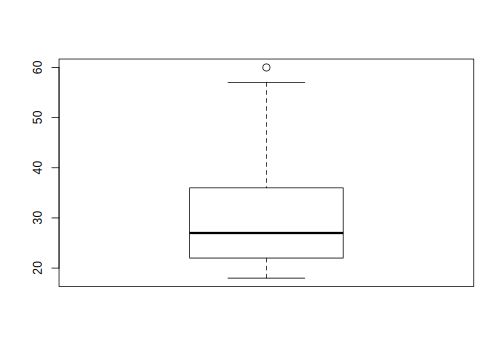
\includegraphics{mtec_cadi_2017_files/figure-latex/unnamed-chunk-38-1.pdf}

\begin{Shaded}
\begin{Highlighting}[]
\CommentTok{# can we do the same stratified by sex?}
\KeywordTok{boxplot}\NormalTok{(arrest_tab}\OperatorTok{$}\NormalTok{age[mount_washington_index]}\OperatorTok{~}\NormalTok{arrest_tab}\OperatorTok{$}\NormalTok{sex[mount_washington_index])}
\end{Highlighting}
\end{Shaded}

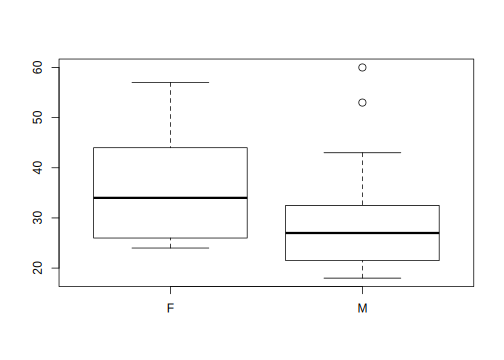
\includegraphics{mtec_cadi_2017_files/figure-latex/unnamed-chunk-38-2.pdf}

This used a very useful notation in R: the tilde,
\texttt{\textasciitilde{}} which we will encounter in a few different
places. One way of thinking about that abstractly is, do something with
this attribute, as a function (or depending on, stratified by,
conditioned on) this other attribute. For instance, ``plot \texttt{age}
as a function of sex'' in our example.

Let's write code that's a little cleaner for that last plot, and let's
also make the plot a bit more useful by adding a title and axis labels:

\begin{Shaded}
\begin{Highlighting}[]
\NormalTok{mount_washington_tab <-}\StringTok{ }\NormalTok{arrest_tab[mount_washington_index,]}
\KeywordTok{boxplot}\NormalTok{(mount_washington_tab}\OperatorTok{$}\NormalTok{age}\OperatorTok{~}\NormalTok{mount_washington_tab}\OperatorTok{$}\NormalTok{sex,}
        \DataTypeTok{main=}\StringTok{"Mt. Washington"}\NormalTok{, }
        \DataTypeTok{xlab=}\StringTok{"Sex"}\NormalTok{, }\DataTypeTok{ylab=}\StringTok{"Arrest Age"}\NormalTok{)}
\end{Highlighting}
\end{Shaded}

\includegraphics{mtec_cadi_2017_files/figure-latex/unnamed-chunk-39-1.pdf}

Here's one more useful plot:

\begin{Shaded}
\begin{Highlighting}[]
\KeywordTok{barplot}\NormalTok{(}\KeywordTok{table}\NormalTok{(mount_washington_tab}\OperatorTok{$}\NormalTok{race), }
        \DataTypeTok{xlab=}\StringTok{"Number of Arrests"}\NormalTok{,}
        \DataTypeTok{ylab=}\StringTok{"Race"}\NormalTok{)}
\end{Highlighting}
\end{Shaded}

\includegraphics{mtec_cadi_2017_files/figure-latex/unnamed-chunk-40-1.pdf}

\section{Functions}\label{functions}

Now suppose we wanted to do a similar analysis for other neighborhoods.
In that case we should encapsulate the summaries and plots we want to do
in a function:

\begin{Shaded}
\begin{Highlighting}[]
\NormalTok{analyze_neighborhood <-}\StringTok{ }\ControlFlowTok{function}\NormalTok{(neighborhood) \{}
\NormalTok{  neighborhood_index <-}\StringTok{ }\NormalTok{arrest_tab}\OperatorTok{$}\NormalTok{neighborhood }\OperatorTok{==}\StringTok{ }\NormalTok{neighborhood}
\NormalTok{  neighborhood_tab <-}\StringTok{ }\NormalTok{arrest_tab[neighborhood_index,]}
  
    \KeywordTok{boxplot}\NormalTok{(neighborhood_tab}\OperatorTok{$}\NormalTok{age}\OperatorTok{~}\NormalTok{neighborhood_tab}\OperatorTok{$}\NormalTok{sex,}
            \DataTypeTok{main =}\NormalTok{ neighborhood,}
            \DataTypeTok{xlab =} \StringTok{"Sex"}\NormalTok{, }\DataTypeTok{ylab=}\StringTok{"Arrest Age"}\NormalTok{)}
    
    \KeywordTok{barplot}\NormalTok{(}\KeywordTok{table}\NormalTok{(neighborhood_tab}\OperatorTok{$}\NormalTok{race),}
            \DataTypeTok{main =}\NormalTok{ neighborhood,}
            \DataTypeTok{xlab =} \StringTok{"Race"}\NormalTok{, }\DataTypeTok{ylab=}\StringTok{"Number of Arrests"}\NormalTok{)}
\NormalTok{\}}
\end{Highlighting}
\end{Shaded}

Now we can use that function to make our plots for specific
neighborhoods

\begin{Shaded}
\begin{Highlighting}[]
\KeywordTok{analyze_neighborhood}\NormalTok{(}\StringTok{"Mount Washington"}\NormalTok{)}
\end{Highlighting}
\end{Shaded}

\includegraphics{mtec_cadi_2017_files/figure-latex/unnamed-chunk-42-1.pdf}
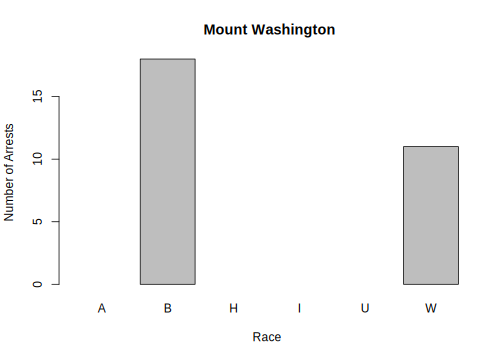
\includegraphics{mtec_cadi_2017_files/figure-latex/unnamed-chunk-42-2.pdf}

\begin{Shaded}
\begin{Highlighting}[]
\KeywordTok{analyze_neighborhood}\NormalTok{(}\StringTok{"Hampden"}\NormalTok{)}
\end{Highlighting}
\end{Shaded}

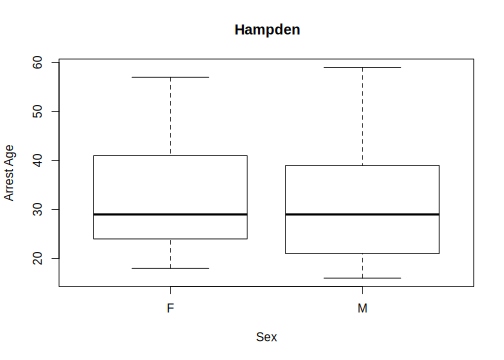
\includegraphics{mtec_cadi_2017_files/figure-latex/unnamed-chunk-42-3.pdf}
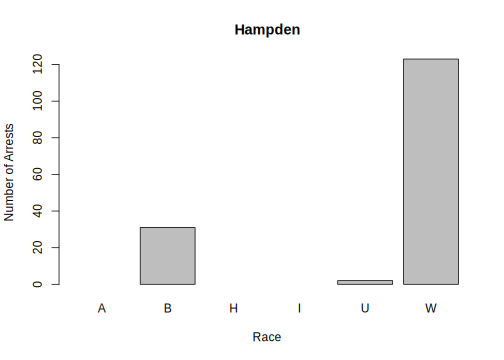
\includegraphics{mtec_cadi_2017_files/figure-latex/unnamed-chunk-42-4.pdf}

\section{A note on data types}\label{a-note-on-data-types}

This dataset contains data of types commonly found in data analyses

\begin{itemize}
\tightlist
\item
  Numeric (continuous): A numeric measurement (e.g., height)\\
\item
  Numeric (discrete): Usually obtained from counting, think only
  integers (e.g., \texttt{age} which is measured in years)\\
\item
  Categorical: One of a possible set of values (e.g., \texttt{sex})\\
\item
  Datetime: Date and time of some event or observation (e.g.,
  \texttt{arrestDate}, \texttt{arrestTime})\\
\item
  geolocation: Latitude and Longitude of some event or observation
  (e.g., \texttt{Location.})
\end{itemize}

The distinction between continuous and discrete is a bit tricky since
measurements that have finite precision must be discrete. So, the
difference really comes up when we build statistical models of datasets
for analysis. For now, think of discrete data as the result of counting,
and continuous data the result of some physical measurement.

We said that R is designed for data analysis. My favorite example of how
that manifests itself is the \texttt{factor} datatype. If you look at
your dataset now, \texttt{arrest\_tab\$sex} is a vector of strings:

\begin{Shaded}
\begin{Highlighting}[]
\KeywordTok{class}\NormalTok{(arrest_tab}\OperatorTok{$}\NormalTok{sex)}
\end{Highlighting}
\end{Shaded}

\begin{verbatim}
## [1] "factor"
\end{verbatim}

\begin{Shaded}
\begin{Highlighting}[]
\KeywordTok{summary}\NormalTok{(arrest_tab}\OperatorTok{$}\NormalTok{sex)}
\end{Highlighting}
\end{Shaded}

\begin{verbatim}
##     F     M  NA's 
## 19431 85095     2
\end{verbatim}

However, as a measurement, or attribute, it should only take one of two
values (or three depending on how you record missing, unknown or
unspecified). So, in R, that categorical data type is called a
\emph{factor}. Notice what the \texttt{summary} function does after
turning the \texttt{sex} attribute into a \emph{factor}:

\begin{Shaded}
\begin{Highlighting}[]
\NormalTok{arrest_tab}\OperatorTok{$}\NormalTok{sex <-}\StringTok{ }\KeywordTok{factor}\NormalTok{(arrest_tab}\OperatorTok{$}\NormalTok{sex)}
\KeywordTok{summary}\NormalTok{(arrest_tab}\OperatorTok{$}\NormalTok{sex)}
\end{Highlighting}
\end{Shaded}

\begin{verbatim}
##     F     M  NA's 
## 19431 85095     2
\end{verbatim}

This distinction shows up in many other places where functions have very
different behavior when called on a vector of strings and when called on
a factor (e.g., functions that make plots, or functions that learn
statistical models).

One last note, the possible values a \emph{factor} can take are called
\emph{levels}:

\begin{Shaded}
\begin{Highlighting}[]
\KeywordTok{levels}\NormalTok{(arrest_tab}\OperatorTok{$}\NormalTok{sex)}
\end{Highlighting}
\end{Shaded}

\begin{verbatim}
## [1] "F" "M"
\end{verbatim}

Exercise: you should transform the \texttt{race} attribute into a factor
as well. How many levels does it have?

\section{Thinking in vectors}\label{thinking-in-vectors}

In data analysis the \emph{vector} is probably the most fundamental data
type (other than basic numbers, strings, etc.). Why? Consider getting
data about one attribute, say height, for a group of people. What do you
get, an array of numbers, all in the same unit (say feet, inches or
centimeters). How about their name? Then you get an array of strings.
Abstractly, we think of vectors as arrays of values, all of the same
\emph{class} or datatype.

In our dataset, each column, corresponding to an attribute, is a vector:

\begin{Shaded}
\begin{Highlighting}[]
\CommentTok{# the 'str' function gives a bit more low-level information about objects}
\KeywordTok{str}\NormalTok{(arrest_tab}\OperatorTok{$}\NormalTok{Location)}
\end{Highlighting}
\end{Shaded}

\begin{verbatim}
## Warning: Unknown or uninitialised column: 'Location'.
\end{verbatim}

\begin{verbatim}
##  NULL
\end{verbatim}

R (and other data analysis languages) are designed to operate on vectors
easily. For example, frequently we want to do some kind of
transformation to a data attribute, say record age in months rather than
years. Then we would perform the \textbf{same operation} for every value
in the corresponding vector:

\begin{Shaded}
\begin{Highlighting}[]
\NormalTok{age_in_months <-}\StringTok{ }\NormalTok{arrest_tab}\OperatorTok{$}\NormalTok{age }\OperatorTok{*}\StringTok{ }\DecValTok{12}
\end{Highlighting}
\end{Shaded}

In a language that doesn't support this type of vectorized operation,
you would use a loop, or similar construct, to perform this operation.

Another type of transformation frequently done is to combine attributes
into a single attribute. Suppose we wanted to combine the
\texttt{arrestLocation} and \texttt{neighborhood} attributes into an
\texttt{address} attribute:

\begin{Shaded}
\begin{Highlighting}[]
\CommentTok{# remember you can always find out what a function does by using ?paste}
\KeywordTok{head}\NormalTok{(}\KeywordTok{paste}\NormalTok{(arrest_tab}\OperatorTok{$}\NormalTok{arrestLocation, arrest_tab}\OperatorTok{$}\NormalTok{neighborhood, }\DataTypeTok{sep=}\StringTok{", "}\NormalTok{))}
\end{Highlighting}
\end{Shaded}

\begin{verbatim}
## [1] "NA, NA"                                   
## [2] "2000 Wilkens Ave, Carrollton Ridge"       
## [3] "2800 Mayfield Ave, Belair-Edison"         
## [4] "2100 Ashburton St, Panway/Braddish Avenue"
## [5] "4000 Wilsby Ave, Pen Lucy"                
## [6] "2900 Spellman Rd, Cherry Hill"
\end{verbatim}

Here the \texttt{paste} function concatenates strings element-wise: the
first string in \texttt{arrestLocation} is concatenated with the first
string in \texttt{neighborhood}, etc.

Arithmetic operations have the same element-wise operation:

\begin{Shaded}
\begin{Highlighting}[]
\CommentTok{# add first 10 odd numbers to first 10 even numbers}
\KeywordTok{seq}\NormalTok{(}\DecValTok{1}\NormalTok{, }\DecValTok{20}\NormalTok{, }\DataTypeTok{by=}\DecValTok{2}\NormalTok{) }\OperatorTok{+}\StringTok{ }\KeywordTok{seq}\NormalTok{(}\DecValTok{2}\NormalTok{, }\DecValTok{20}\NormalTok{, }\DataTypeTok{by=}\DecValTok{2}\NormalTok{)}
\end{Highlighting}
\end{Shaded}

\begin{verbatim}
##  [1]  3  7 11 15 19 23 27 31 35 39
\end{verbatim}

\section{Lists vs.~vectors}\label{lists-vs.vectors}

We saw that vectors are arrays of values, all of the same \emph{class}.
R also allows arrays of values that have different \emph{class} or
datatype. These are called \emph{lists}. Here is a list containing a
string, and a couple of numbers:

\begin{Shaded}
\begin{Highlighting}[]
\NormalTok{my_list <-}\StringTok{ }\KeywordTok{list}\NormalTok{(}\StringTok{"Hector"}\NormalTok{, }\DecValTok{40}\NormalTok{, }\DecValTok{71}\NormalTok{)}
\NormalTok{my_list}
\end{Highlighting}
\end{Shaded}

\begin{verbatim}
## [[1]]
## [1] "Hector"
## 
## [[2]]
## [1] 40
## 
## [[3]]
## [1] 71
\end{verbatim}

Indexing in lists uses different syntax from the indexing we saw before.
To index an element in a list we would use a double-bracket
\texttt{{[}{[}}.

\begin{Shaded}
\begin{Highlighting}[]
\NormalTok{my_list[[}\DecValTok{1}\NormalTok{]]}
\end{Highlighting}
\end{Shaded}

\begin{verbatim}
## [1] "Hector"
\end{verbatim}

In contrast, the single bracket \texttt{{[}} indexes a \emph{part} of
the list, and thus returns another list.

\begin{Shaded}
\begin{Highlighting}[]
\NormalTok{my_list[}\DecValTok{1}\NormalTok{]}
\end{Highlighting}
\end{Shaded}

\begin{verbatim}
## [[1]]
## [1] "Hector"
\end{verbatim}

That way we can use slice notation and other operations we saw when
indexing vectors as before, but we get lists as results.

\begin{Shaded}
\begin{Highlighting}[]
\NormalTok{my_list[}\DecValTok{1}\OperatorTok{:}\DecValTok{2}\NormalTok{]}
\end{Highlighting}
\end{Shaded}

\begin{verbatim}
## [[1]]
## [1] "Hector"
## 
## [[2]]
## [1] 40
\end{verbatim}

List elements can have names as well:

\begin{Shaded}
\begin{Highlighting}[]
\NormalTok{named_list <-}\StringTok{ }\KeywordTok{list}\NormalTok{(}\DataTypeTok{person=}\StringTok{"Hector"}\NormalTok{, }\DataTypeTok{age=}\DecValTok{40}\NormalTok{, }\DataTypeTok{height=}\DecValTok{71}\NormalTok{)}
\NormalTok{named_list}
\end{Highlighting}
\end{Shaded}

\begin{verbatim}
## $person
## [1] "Hector"
## 
## $age
## [1] 40
## 
## $height
## [1] 71
\end{verbatim}

Which we can use to index elements as well (both with \texttt{{[}{[}}
and \texttt{\$})

\begin{Shaded}
\begin{Highlighting}[]
\NormalTok{named_list[[}\StringTok{"person"}\NormalTok{]]}
\end{Highlighting}
\end{Shaded}

\begin{verbatim}
## [1] "Hector"
\end{verbatim}

\begin{Shaded}
\begin{Highlighting}[]
\NormalTok{named_list}\OperatorTok{$}\NormalTok{person}
\end{Highlighting}
\end{Shaded}

\begin{verbatim}
## [1] "Hector"
\end{verbatim}

Lists can hold arbitrary objects as elements. For example you can have a
vector of strings as an element in a list

\begin{Shaded}
\begin{Highlighting}[]
\NormalTok{my_list <-}\StringTok{ }\KeywordTok{list}\NormalTok{(}\DataTypeTok{person=}\KeywordTok{c}\NormalTok{(}\StringTok{"Hector"}\NormalTok{, }\StringTok{"Ringo"}\NormalTok{, }\StringTok{"Paul"}\NormalTok{, }\StringTok{"John"}\NormalTok{), }\DecValTok{40}\NormalTok{, }\DecValTok{71}\NormalTok{)}
\NormalTok{my_list}
\end{Highlighting}
\end{Shaded}

\begin{verbatim}
## $person
## [1] "Hector" "Ringo"  "Paul"   "John"  
## 
## [[2]]
## [1] 40
## 
## [[3]]
## [1] 71
\end{verbatim}

Now, we come to a momentous occassion in understanding R.
\texttt{data.frame}s are special instances of \emph{lists}! But, in this
case, every element in the list is a vector, and all vectors have
exactly the same length. So \texttt{arrest\_tab\$age} indexes the named
element \texttt{age} in the list \texttt{arrest\_tab}!

The pattern of \emph{applying} functions to entries in vectors also
holds for elements in lists. So, if we want to calculate smallest value
for every attribute in our dataset, we could do something like this:

\begin{Shaded}
\begin{Highlighting}[]
\KeywordTok{sapply}\NormalTok{(arrest_tab, }\ControlFlowTok{function}\NormalTok{(v) }\KeywordTok{sort}\NormalTok{(v)[}\DecValTok{1}\NormalTok{])}
\end{Highlighting}
\end{Shaded}

\begin{verbatim}
##                                           arrest 
##                                       "11126858" 
##                                              age 
##                                              "0" 
##                                             race 
##                                              "1" 
##                                              sex 
##                                              "1" 
##                                       arrestDate 
##                                     "01/01/2011" 
##                                       arrestTime 
##                                              "0" 
##                                   arrestLocation 
##                                      "0 20Th St" 
##                                  incidentOffense 
##                                              "1" 
##                                 incidentLocation 
##                        "*** District Detail ***" 
##                                           charge 
##                                         "1 0002" 
##                                chargeDescription 
## "Abduct Child Under 12 || Abduct Child Under 12" 
##                                         district 
##                                        "CENTRAL" 
##                                             post 
##                                            "111" 
##                                     neighborhood 
##                                          "Abell" 
##                                       Location 1 
##                "(39.2000327685, -76.5555163146)"
\end{verbatim}

\section{Making the process explicit with
pipes}\label{making-the-process-explicit-with-pipes}

We've discussed the idea of thinking about data analysis work in terms
of ``pipelines'', where we start from data of a certain shape (e.g., a
\texttt{data.frame}) and apply transformations (functions) to obtain
data that contains the computation we want. Consider the following
example seen in class:

\emph{What is the mean age of males arrested in the SOUTHERN district?}

We can frame the answer to this question as a series of data
transformations to get the answer we are looking for:

\begin{Shaded}
\begin{Highlighting}[]
\CommentTok{# filter data to observations we need}
\NormalTok{index_vector <-}\StringTok{ }\NormalTok{arrest_tab}\OperatorTok{$}\NormalTok{sex }\OperatorTok{==}\StringTok{ "M"} \OperatorTok{&}\StringTok{ }\NormalTok{arrest_tab}\OperatorTok{$}\NormalTok{district }\OperatorTok{==}\StringTok{ "SOUTHERN"}
\NormalTok{tmp <-}\StringTok{ }\NormalTok{arrest_tab[index_vector,]}

\CommentTok{# select the attribute/column we need}
\NormalTok{tmp <-}\StringTok{ }\NormalTok{tmp[[}\StringTok{"age"}\NormalTok{]]}

\CommentTok{# compute statistic required}
\KeywordTok{mean}\NormalTok{(tmp, }\DataTypeTok{na.rm=}\OtherTok{TRUE}\NormalTok{)}
\end{Highlighting}
\end{Shaded}

\begin{verbatim}
## [1] 32.28481
\end{verbatim}

Let's rewrite this using functions to illustrate the point

\begin{Shaded}
\begin{Highlighting}[]
\NormalTok{filter_data <-}\StringTok{ }\ControlFlowTok{function}\NormalTok{(data) \{}
\NormalTok{  index_vector <-}\StringTok{ }\NormalTok{data}\OperatorTok{$}\NormalTok{sex }\OperatorTok{==}\StringTok{ "M"} \OperatorTok{&}\StringTok{ }\NormalTok{data}\OperatorTok{$}\NormalTok{district }\OperatorTok{==}\StringTok{ "SOUTHERN"}
\NormalTok{  data[index_vector,]}
\NormalTok{\}}

\NormalTok{select_column <-}\StringTok{ }\ControlFlowTok{function}\NormalTok{(data, column) \{}
\NormalTok{  data[[column]]}
\NormalTok{\}}

\NormalTok{tmp <-}\StringTok{ }\KeywordTok{filter_data}\NormalTok{(arrest_tab)}
\NormalTok{tmp <-}\StringTok{ }\KeywordTok{select_column}\NormalTok{(tmp, }\StringTok{"age"}\NormalTok{)}
\KeywordTok{mean}\NormalTok{(tmp, }\DataTypeTok{na.rm=}\OtherTok{TRUE}\NormalTok{)}
\end{Highlighting}
\end{Shaded}

\begin{verbatim}
## [1] 32.28481
\end{verbatim}

So, this pattern of
\emph{data--\textgreater{}transform--\textgreater{}data} becomes clearer
when written that way.

The \texttt{dplyr} package introduces \emph{syntactic sugar} to make
this explicit. We can write the above snippet using the ``pipe''
operator \texttt{\%\textgreater{}\%}:

\begin{Shaded}
\begin{Highlighting}[]
\NormalTok{arrest_tab }\OperatorTok
\StringTok{  }\KeywordTok{filter_data}\NormalTok{() }\OperatorTok
\StringTok{  }\KeywordTok{select_column}\NormalTok{(}\StringTok{"age"}\NormalTok{) }\OperatorTok
\StringTok{  }\KeywordTok{mean}\NormalTok{(}\DataTypeTok{na.rm=}\OtherTok{TRUE}\NormalTok{)}
\end{Highlighting}
\end{Shaded}

\begin{verbatim}
## [1] 32.28481
\end{verbatim}

The \texttt{\%\textgreater{}\%} binary operator takes the value to its
\textbf{left} and inserts it as the first argument of the function call
to its \textbf{right}. So the expression
\texttt{LHS\ \%\textgreater{}\%\ f(another\_argument)} is
\textbf{equivalent} to the expression
\texttt{f(LHS,\ another\_argument)}. We will see this pattern
extensively in class because it explicitly presents the way we want to
organize many of our data analysis tasks.

\chapter{Ingesting data}\label{ingesting-data}

Now that we have a better understanding of the R data analysis language,
we turn to the first significant challenge in data analysis, getting
data into R in a shape that we can use to start our analysis. We will
look at two types of data ingestion: \emph{structured ingestion}, where
we read data that is already structured, like a comma separated value
(CSV) file, and \emph{scraping} where we obtain data from text, usually
in websites.

\section{Structured ingestion}\label{structured-ingestion}

\subsection{CSV files (and similar)}\label{csv-files-and-similar}

We saw in a previous chapter how we can use the \texttt{read\_csv} file
to read data from a CSV file into a data frame. Comma separated value
(CSV) files are structured in a somewhat regular way, so reading into a
data frame is straightforward. Each line in the CSV file corresponds to
an observation (a row in a data frame). Each line contains values
separated by a comma (\texttt{,}), corresponding to the variables of
each observation.

This ideal principle of how a CSV file is constructed is frequently
violated by data contained in CSV files. To get a sense of how to deal
with these cases look at the documentation of the \texttt{read\_csv}
function. For instance:

\begin{itemize}
\item
  the first line of the file may or may not contain the names of
  variables for the data frame (\texttt{col\_names} argument).
\item
  strings are quoted using \texttt{\textquotesingle{}} instead of
  \texttt{"} (\texttt{quote} argument)
\item
  missing data is encoded with a non-standard code, e.g., \texttt{-}
  (\texttt{na} argument)
\item
  values are separated by a character other than \texttt{,}
  (\texttt{read\_delim} function)
\item
  file may contain header information before the actual data so we have
  to skip some lines when loading the data (\texttt{skip} argument)
\end{itemize}

You should read the documentation of the \texttt{read\_csv} function to
appreciate the complexities it can maneuver when reading data from
structured text files.

\begin{Shaded}
\begin{Highlighting}[]
\NormalTok{?read_csv}
\end{Highlighting}
\end{Shaded}

\subsection{Excel spreadsheets}\label{excel-spreadsheets}

Often you will need to ingest data that is stored in an Excel
spreadsheet. The \texttt{readxl} package is used to do this. The main
function for this package is the \texttt{read\_excel} function. It
contains similar arguments to the \texttt{read\_csv} function we saw
above.

\textbf{On your own:} Use the \texttt{read\_excel} function to parse
migration data from the 2009 INEGI national survey contained in file
\texttt{data/Migracion\_interna\_eua.xls}.

\section{Scraping}\label{scraping}

Often, data we want to use is hosted as part of HTML files in webpages.
The markup structure of HTML allows to parse data into tables we can use
for analysis. Let's use the Rotten Tomatoes ratings webpage for Diego
Luna as an example:

\begin{figure}
\centering
\includegraphics{img/rt_diegoluna.png}
\caption{}
\end{figure}

We can scrape ratings for his movies from this page. To do this we need
to figure out how the HTML page's markup can help us write R expressions
to find this data in the page. Most web browsers have facilities to show
page markup. In Google Chrome, you can use
\texttt{View\textgreater{}Developer\textgreater{}Developer\ Tools}, and
inspect the page markdown to find where the data is contained. In this
example, we see that the data we want is in a
\texttt{\textless{}table\textgreater{}} element in the page, with id
\texttt{filmographyTbl}.

\begin{figure}
\centering
\includegraphics{img/rt_devtools.png}
\caption{}
\end{figure}

Now that we have that information, we can use the \texttt{rvest} package
to scrape this data:

\begin{Shaded}
\begin{Highlighting}[]
\KeywordTok{library}\NormalTok{(rvest)}

\NormalTok{url <-}\StringTok{ "https://www.rottentomatoes.com/celebrity/diego_luna"}

\NormalTok{dl_tab <-}\StringTok{ }\NormalTok{url }\OperatorTok
\StringTok{  }\KeywordTok{read_html}\NormalTok{() }\OperatorTok
\StringTok{  }\KeywordTok{html_node}\NormalTok{(}\StringTok{"#filmographyTbl"}\NormalTok{) }\OperatorTok
\StringTok{  }\KeywordTok{html_table}\NormalTok{()}

\KeywordTok{head}\NormalTok{(dl_tab)}
\end{Highlighting}
\end{Shaded}

\begin{verbatim}
##         RATING                        TITLE
## 1 No Score Yet                   Flatliners
## 2          85% Rogue One: A Star Wars Story
## 3          89%                 Blood Father
## 4          62%            Mr. Pig (Sr. Pig)
## 5          82%             The Book of Life
## 6          39%                 Cesar Chavez
##                                                                                                                                                                                                                                                                                                     CREDIT
## 1                                                                                                                                                                                                                                                                                                      Ray
## 2                                                                                                                                                                                                                                                                                    Captain Cassian Andor
## 3                                                                                                                                                                                                                                                                                                    Jonah
## 4 Producer\n                                                \n                                    \n                                            Screenwriter\n                                                \n                                    \n                                            Director
## 5                                                                                                                                                                                                                                                                                                   Manolo
## 6                                                                                                                                                   Producer\n                                                \n                                    \n                                            Director
##   BOX OFFICE YEAR
## 1          — 2017
## 2    $532.2M 2016
## 3          — 2016
## 4          — 2016
## 5          — 2014
## 6      $5.6M 2014
\end{verbatim}

The main two functions we used here are \texttt{html\_node} and
\texttt{html\_table}. \texttt{html\_node} finds elements in the HTML
page according to some selection criteria. Since we want the element
with \texttt{id=filmographyTbl} we use the \texttt{\#} selection
operation since that corresponds to selection by id. Once the desired
element in the page is selected, we can use the \texttt{html\_table}
function to parse the element's text into a data frame.

\textbf{On your own:} If you wanted to extract the TV filmography from
the page, how would you change this call?

\textbf{On your own:} We can get movie budget and gross information from
this page: \url{http://www.the-numbers.com/movie/budgets/all}. Write R
code to scrape the budget data from that page.

\chapter{Tidying data}\label{tidying-data}

This section is concerned with common problems in data preparation,
namely use cases commonly found in raw datasets that need to be
addressed to turn messy data into tidy data. These would be operations
that you would perform on data obtained as a csv file from a
collaborator or data repository, or as the result of scraping data from
webpages or other sources. We derive many of our ideas from the paper
\href{http://www.jstatsoft.org/v59/i10/paper}{Tidy Data} by Hadley
Wickham. Associated with that paper we will use two very powerful R
libraries \texttt{tidyr} and \texttt{dplyr} which are extremely useful
in writing scripts for data cleaning, preparation and summarization. A
basic design principle behind these libraries is trying to effectively
and efficiently capture very common use cases and operations performed
in data cleaning. The paper frames these use cases and operations which
are them implemented in software.

\section{Tidy Data}\label{tidy-data}

Here we assume we are working with a data model based on rectangular
data structures where

\begin{enumerate}
\def\labelenumi{\arabic{enumi}.}
\tightlist
\item
  Each attribute (or variable) forms a column\\
\item
  Each entity (or observation) forms a row\\
\item
  Each type of entity (observational unit) forms a table
\end{enumerate}

Here is an example of a tidy dataset:

\begin{Shaded}
\begin{Highlighting}[]
\KeywordTok{library}\NormalTok{(nycflights13)}
\KeywordTok{head}\NormalTok{(flights)}
\end{Highlighting}
\end{Shaded}

\begin{verbatim}
## # A tibble: 6 x 19
##    year month   day dep_time sched_dep_time dep_delay arr_time
##   <int> <int> <int>    <int>          <int>     <dbl>    <int>
## 1  2013     1     1      517            515      2.00      830
## 2  2013     1     1      533            529      4.00      850
## 3  2013     1     1      542            540      2.00      923
## 4  2013     1     1      544            545     -1.00     1004
## 5  2013     1     1      554            600     -6.00      812
## 6  2013     1     1      554            558     -4.00      740
## # ... with 12 more variables: sched_arr_time <int>, arr_delay <dbl>,
## #   carrier <chr>, flight <int>, tailnum <chr>, origin <chr>, dest <chr>,
## #   air_time <dbl>, distance <dbl>, hour <dbl>, minute <dbl>, time_hour
## #   <dttm>
\end{verbatim}

it has one observation per row, a single variable per column. Notice
only information about flights are included here (e.g., no airport
information other than the name) in these observations.

\section{Common problems in messy
data}\label{common-problems-in-messy-data}

The set of common operations we will study are based on these common
problems found in datasets. We will see each one in detail:

\begin{itemize}
\tightlist
\item
  Column headers are values, not variable names (gather)\\
\item
  Multiple variables stored in one column (split)\\
\item
  Variables stored in both rows and column (rotate)\\
\item
  Multiple types of observational units are stored in the same table
  (normalize)\\
\item
  Single observational unit stored in multiple tables (join)
\end{itemize}

We are using data from Hadley's paper found in
\href{https://github.com/hadley/tidyr}{github}. It's included directory
\texttt{data}:

\begin{Shaded}
\begin{Highlighting}[]
\NormalTok{data_dir <-}\StringTok{ "data"}
\end{Highlighting}
\end{Shaded}

\subsection{Headers as values}\label{headers-as-values}

The first problem we'll see is the case where a table header contains
values. At this point we will introduce the \texttt{dplyr} package,
which we'll use extensively in this course. It is an extremely powerful
and efficient way of manipulating tidy data. It will serve as the core
of our data manipulation knowledge after this course.

\texttt{dplyr} defines a slightly different way of using data.frames.
The \texttt{tbl\_df} function converts a standard R data.frame into a
\texttt{tbl\_df} defined by \texttt{dplyr}. One nice thing it does, for
example, is print tables in a much friendlier way.

\begin{Shaded}
\begin{Highlighting}[]
\KeywordTok{library}\NormalTok{(tidyr)}
\KeywordTok{library}\NormalTok{(dplyr)}
\KeywordTok{library}\NormalTok{(readr)}

\NormalTok{pew <-}\StringTok{ }\KeywordTok{read_csv}\NormalTok{(}\KeywordTok{file.path}\NormalTok{(data_dir, }\StringTok{"pew.csv"}\NormalTok{))}
\end{Highlighting}
\end{Shaded}

\begin{verbatim}
## Parsed with column specification:
## cols(
##   religion = col_character(),
##   `<$10k` = col_integer(),
##   `$10-20k` = col_integer(),
##   `$20-30k` = col_integer(),
##   `$30-40k` = col_integer(),
##   `$40-50k` = col_integer(),
##   `$50-75k` = col_integer(),
##   `$75-100k` = col_integer(),
##   `$100-150k` = col_integer(),
##   `>150k` = col_integer(),
##   `Don't know/refused` = col_integer()
## )
\end{verbatim}

\begin{Shaded}
\begin{Highlighting}[]
\NormalTok{pew}
\end{Highlighting}
\end{Shaded}

\begin{verbatim}
## # A tibble: 18 x 11
##    religion      `<$10k` `$10-20k` `$20-30k` `$30-40k` `$40-50k` `$50-75k`
##    <chr>           <int>     <int>     <int>     <int>     <int>     <int>
##  1 Agnostic           27        34        60        81        76       137
##  2 Atheist            12        27        37        52        35        70
##  3 Buddhist           27        21        30        34        33        58
##  4 Catholic          418       617       732       670       638      1116
##  5 Don’t know/r~      15        14        15        11        10        35
##  6 Evangelical ~     575       869      1064       982       881      1486
##  7 Hindu               1         9         7         9        11        34
##  8 Historically~     228       244       236       238       197       223
##  9 Jehovah's Wi~      20        27        24        24        21        30
## 10 Jewish             19        19        25        25        30        95
## 11 Mainline Prot     289       495       619       655       651      1107
## 12 Mormon             29        40        48        51        56       112
## 13 Muslim              6         7         9        10         9        23
## 14 Orthodox           13        17        23        32        32        47
## 15 Other Christ~       9         7        11        13        13        14
## 16 Other Faiths       20        33        40        46        49        63
## 17 Other World ~       5         2         3         4         2         7
## 18 Unaffiliated      217       299       374       365       341       528
## # ... with 4 more variables: `$75-100k` <int>, `$100-150k` <int>, `>150k`
## #   <int>, `Don't know/refused` <int>
\end{verbatim}

This table has the number of survey respondents of a specific religion
that report their income within some range. A tidy version of this table
would consider the \emph{variables} of each observation to be
\texttt{religion,\ income,\ frequency} where \texttt{frequency} has the
number of respondents for each religion and income range. The function
to use in the \texttt{tidyr} package is \texttt{gather}:

\begin{Shaded}
\begin{Highlighting}[]
\NormalTok{tidy_pew <-}\StringTok{ }\KeywordTok{gather}\NormalTok{(pew, income, frequency, }\OperatorTok{-}\NormalTok{religion)}
\NormalTok{tidy_pew}
\end{Highlighting}
\end{Shaded}

\begin{verbatim}
## # A tibble: 180 x 3
##    religion                income frequency
##    <chr>                   <chr>      <int>
##  1 Agnostic                <$10k         27
##  2 Atheist                 <$10k         12
##  3 Buddhist                <$10k         27
##  4 Catholic                <$10k        418
##  5 Don’t know/refused      <$10k         15
##  6 Evangelical Prot        <$10k        575
##  7 Hindu                   <$10k          1
##  8 Historically Black Prot <$10k        228
##  9 Jehovah's Witness       <$10k         20
## 10 Jewish                  <$10k         19
## # ... with 170 more rows
\end{verbatim}

This says: gather all the columns from the \texttt{pew} (except
\texttt{religion}) into key-value columns \texttt{income} and
\texttt{frequency}. This table is much easier to use in other analyses.

Another example: this table has a row for each song appearing in the
billboard top 100. It contains track information, and the date it
entered the top 100. It then shows the rank in each of the next 76
weeks.

\begin{Shaded}
\begin{Highlighting}[]
\NormalTok{billboard <-}\StringTok{ }\KeywordTok{read_csv}\NormalTok{(}\KeywordTok{file.path}\NormalTok{(data_dir, }\StringTok{"billboard.csv"}\NormalTok{))}
\end{Highlighting}
\end{Shaded}

\begin{verbatim}
## Parsed with column specification:
## cols(
##   .default = col_integer(),
##   artist = col_character(),
##   track = col_character(),
##   time = col_time(format = ""),
##   date.entered = col_date(format = ""),
##   wk66 = col_character(),
##   wk67 = col_character(),
##   wk68 = col_character(),
##   wk69 = col_character(),
##   wk70 = col_character(),
##   wk71 = col_character(),
##   wk72 = col_character(),
##   wk73 = col_character(),
##   wk74 = col_character(),
##   wk75 = col_character(),
##   wk76 = col_character()
## )
\end{verbatim}

\begin{verbatim}
## See spec(...) for full column specifications.
\end{verbatim}

\begin{Shaded}
\begin{Highlighting}[]
\NormalTok{billboard}
\end{Highlighting}
\end{Shaded}

\begin{verbatim}
## # A tibble: 317 x 81
##     year artist   track   time  date.entered   wk1   wk2   wk3   wk4   wk5
##    <int> <chr>    <chr>   <tim> <date>       <int> <int> <int> <int> <int>
##  1  2000 2 Pac    Baby D~ 04:22 2000-02-26      87    82    72    77    87
##  2  2000 2Ge+her  The Ha~ 03:15 2000-09-02      91    87    92    NA    NA
##  3  2000 3 Doors~ Krypto~ 03:53 2000-04-08      81    70    68    67    66
##  4  2000 3 Doors~ Loser   04:24 2000-10-21      76    76    72    69    67
##  5  2000 504 Boyz Wobble~ 03:35 2000-04-15      57    34    25    17    17
##  6  2000 98^0     Give M~ 03:24 2000-08-19      51    39    34    26    26
##  7  2000 A*Teens  Dancin~ 03:44 2000-07-08      97    97    96    95   100
##  8  2000 Aaliyah  I Don'~ 04:15 2000-01-29      84    62    51    41    38
##  9  2000 Aaliyah  Try Ag~ 04:03 2000-03-18      59    53    38    28    21
## 10  2000 Adams, ~ Open M~ 05:30 2000-08-26      76    76    74    69    68
## # ... with 307 more rows, and 71 more variables: wk6 <int>, wk7 <int>, wk8
## #   <int>, wk9 <int>, wk10 <int>, wk11 <int>, wk12 <int>, wk13 <int>, wk14
## #   <int>, wk15 <int>, wk16 <int>, wk17 <int>, wk18 <int>, wk19 <int>,
## #   wk20 <int>, wk21 <int>, wk22 <int>, wk23 <int>, wk24 <int>, wk25
## #   <int>, wk26 <int>, wk27 <int>, wk28 <int>, wk29 <int>, wk30 <int>,
## #   wk31 <int>, wk32 <int>, wk33 <int>, wk34 <int>, wk35 <int>, wk36
## #   <int>, wk37 <int>, wk38 <int>, wk39 <int>, wk40 <int>, wk41 <int>,
## #   wk42 <int>, wk43 <int>, wk44 <int>, wk45 <int>, wk46 <int>, wk47
## #   <int>, wk48 <int>, wk49 <int>, wk50 <int>, wk51 <int>, wk52 <int>,
## #   wk53 <int>, wk54 <int>, wk55 <int>, wk56 <int>, wk57 <int>, wk58
## #   <int>, wk59 <int>, wk60 <int>, wk61 <int>, wk62 <int>, wk63 <int>,
## #   wk64 <int>, wk65 <int>, wk66 <chr>, wk67 <chr>, wk68 <chr>, wk69
## #   <chr>, wk70 <chr>, wk71 <chr>, wk72 <chr>, wk73 <chr>, wk74 <chr>,
## #   wk75 <chr>, wk76 <chr>
\end{verbatim}

Challenge: This dataset has values as column names. Which column names
are values? How do we tidy this dataset?

\subsection{Multiple variables in one
column}\label{multiple-variables-in-one-column}

The next problem we'll see is the case when we see multiple variables in
a single column. Consider the following dataset of tuberculosis cases:

\begin{Shaded}
\begin{Highlighting}[]
\NormalTok{tb <-}\StringTok{ }\KeywordTok{read_csv}\NormalTok{(}\KeywordTok{file.path}\NormalTok{(data_dir, }\StringTok{"tb.csv"}\NormalTok{))}
\end{Highlighting}
\end{Shaded}

\begin{verbatim}
## Parsed with column specification:
## cols(
##   .default = col_integer(),
##   iso2 = col_character()
## )
\end{verbatim}

\begin{verbatim}
## See spec(...) for full column specifications.
\end{verbatim}

\begin{Shaded}
\begin{Highlighting}[]
\NormalTok{tb}
\end{Highlighting}
\end{Shaded}

\begin{verbatim}
## # A tibble: 5,769 x 22
##    iso2   year   m04  m514  m014 m1524 m2534 m3544 m4554 m5564   m65    mu
##    <chr> <int> <int> <int> <int> <int> <int> <int> <int> <int> <int> <int>
##  1 AD     1989    NA    NA    NA    NA    NA    NA    NA    NA    NA    NA
##  2 AD     1990    NA    NA    NA    NA    NA    NA    NA    NA    NA    NA
##  3 AD     1991    NA    NA    NA    NA    NA    NA    NA    NA    NA    NA
##  4 AD     1992    NA    NA    NA    NA    NA    NA    NA    NA    NA    NA
##  5 AD     1993    NA    NA    NA    NA    NA    NA    NA    NA    NA    NA
##  6 AD     1994    NA    NA    NA    NA    NA    NA    NA    NA    NA    NA
##  7 AD     1996    NA    NA     0     0     0     4     1     0     0    NA
##  8 AD     1997    NA    NA     0     0     1     2     2     1     6    NA
##  9 AD     1998    NA    NA     0     0     0     1     0     0     0    NA
## 10 AD     1999    NA    NA     0     0     0     1     1     0     0    NA
## # ... with 5,759 more rows, and 10 more variables: f04 <int>, f514 <int>,
## #   f014 <int>, f1524 <int>, f2534 <int>, f3544 <int>, f4554 <int>, f5564
## #   <int>, f65 <int>, fu <int>
\end{verbatim}

This table has a row for each year and strain of tuberculosis (given by
the first two columns). The remaining columns state the number of cases
for a given demographic. For example, \texttt{m1524} corresponds to
males between 15 and 24 years old, and \texttt{f1524} are females age
15-24. As you can see each of these columns has two variables:
\texttt{sex} and \texttt{age}.

Challenge: what else is untidy about this dataset?

So, we have to do two operations to tidy this table, first we need to
use \texttt{gather} the tabulation columns into a \texttt{demo} and
\texttt{n} columns (for demographic and number of cases):

\begin{Shaded}
\begin{Highlighting}[]
\NormalTok{tidy_tb <-}\StringTok{ }\KeywordTok{gather}\NormalTok{(tb, demo, n, }\OperatorTok{-}\NormalTok{iso2, }\OperatorTok{-}\NormalTok{year)}
\NormalTok{tidy_tb}
\end{Highlighting}
\end{Shaded}

\begin{verbatim}
## # A tibble: 115,380 x 4
##    iso2   year demo      n
##    <chr> <int> <chr> <int>
##  1 AD     1989 m04      NA
##  2 AD     1990 m04      NA
##  3 AD     1991 m04      NA
##  4 AD     1992 m04      NA
##  5 AD     1993 m04      NA
##  6 AD     1994 m04      NA
##  7 AD     1996 m04      NA
##  8 AD     1997 m04      NA
##  9 AD     1998 m04      NA
## 10 AD     1999 m04      NA
## # ... with 115,370 more rows
\end{verbatim}

Next, we need to \texttt{separate} the values in the \texttt{demo}
column into two variables \texttt{sex} and \texttt{age}

\begin{Shaded}
\begin{Highlighting}[]
\NormalTok{tidy_tb <-}\StringTok{ }\KeywordTok{separate}\NormalTok{(tidy_tb, demo, }\KeywordTok{c}\NormalTok{(}\StringTok{"sex"}\NormalTok{, }\StringTok{"age"}\NormalTok{), }\DataTypeTok{sep=}\DecValTok{1}\NormalTok{)}
\NormalTok{tidy_tb}
\end{Highlighting}
\end{Shaded}

\begin{verbatim}
## # A tibble: 115,380 x 5
##    iso2   year sex   age       n
##  * <chr> <int> <chr> <chr> <int>
##  1 AD     1989 m     04       NA
##  2 AD     1990 m     04       NA
##  3 AD     1991 m     04       NA
##  4 AD     1992 m     04       NA
##  5 AD     1993 m     04       NA
##  6 AD     1994 m     04       NA
##  7 AD     1996 m     04       NA
##  8 AD     1997 m     04       NA
##  9 AD     1998 m     04       NA
## 10 AD     1999 m     04       NA
## # ... with 115,370 more rows
\end{verbatim}

This calls the \texttt{separate} function on table \texttt{tidy\_db},
separating the \texttt{demo} variable into variables \texttt{sex} and
\texttt{age} by separating each value after the first character (that's
the \texttt{sep} argument).

We can put these two commands together in a pipeline:

\begin{Shaded}
\begin{Highlighting}[]
\NormalTok{tidy_tb <-}\StringTok{ }\NormalTok{tb }\OperatorTok\StringTok{ }
\StringTok{  }\KeywordTok{gather}\NormalTok{(demo, n, }\OperatorTok{-}\NormalTok{iso2, }\OperatorTok{-}\NormalTok{year)  }\OperatorTok
\StringTok{  }\KeywordTok{separate}\NormalTok{(demo, }\KeywordTok{c}\NormalTok{(}\StringTok{"sex"}\NormalTok{, }\StringTok{"age"}\NormalTok{), }\DataTypeTok{sep=}\DecValTok{1}\NormalTok{)}
\NormalTok{tidy_tb}
\end{Highlighting}
\end{Shaded}

\begin{verbatim}
## # A tibble: 115,380 x 5
##    iso2   year sex   age       n
##  * <chr> <int> <chr> <chr> <int>
##  1 AD     1989 m     04       NA
##  2 AD     1990 m     04       NA
##  3 AD     1991 m     04       NA
##  4 AD     1992 m     04       NA
##  5 AD     1993 m     04       NA
##  6 AD     1994 m     04       NA
##  7 AD     1996 m     04       NA
##  8 AD     1997 m     04       NA
##  9 AD     1998 m     04       NA
## 10 AD     1999 m     04       NA
## # ... with 115,370 more rows
\end{verbatim}

\subsection{Variables stored in both rows and
columns}\label{variables-stored-in-both-rows-and-columns}

This is the messiest, commonly found type of data. Let's take a look at
an example, this is daily weather data from for one weather station in
Mexico in 2010.

\begin{Shaded}
\begin{Highlighting}[]
\NormalTok{weather <-}\StringTok{ }\KeywordTok{read_csv}\NormalTok{(}\KeywordTok{file.path}\NormalTok{(data_dir, }\StringTok{"weather.csv"}\NormalTok{))}
\end{Highlighting}
\end{Shaded}

\begin{verbatim}
## Parsed with column specification:
## cols(
##   .default = col_double(),
##   id = col_character(),
##   year = col_integer(),
##   month = col_integer(),
##   element = col_character(),
##   d9 = col_character(),
##   d12 = col_character(),
##   d18 = col_character(),
##   d19 = col_character(),
##   d20 = col_character(),
##   d21 = col_character(),
##   d22 = col_character(),
##   d24 = col_character()
## )
\end{verbatim}

\begin{verbatim}
## See spec(...) for full column specifications.
\end{verbatim}

\begin{Shaded}
\begin{Highlighting}[]
\NormalTok{weather}
\end{Highlighting}
\end{Shaded}

\begin{verbatim}
## # A tibble: 22 x 35
##    id       year month element    d1    d2    d3    d4    d5    d6    d7
##    <chr>   <int> <int> <chr>   <dbl> <dbl> <dbl> <dbl> <dbl> <dbl> <dbl>
##  1 MX17004  2010     1 tmax       NA  NA    NA      NA  NA      NA    NA
##  2 MX17004  2010     1 tmin       NA  NA    NA      NA  NA      NA    NA
##  3 MX17004  2010     2 tmax       NA  27.3  24.1    NA  NA      NA    NA
##  4 MX17004  2010     2 tmin       NA  14.4  14.4    NA  NA      NA    NA
##  5 MX17004  2010     3 tmax       NA  NA    NA      NA  32.1    NA    NA
##  6 MX17004  2010     3 tmin       NA  NA    NA      NA  14.2    NA    NA
##  7 MX17004  2010     4 tmax       NA  NA    NA      NA  NA      NA    NA
##  8 MX17004  2010     4 tmin       NA  NA    NA      NA  NA      NA    NA
##  9 MX17004  2010     5 tmax       NA  NA    NA      NA  NA      NA    NA
## 10 MX17004  2010     5 tmin       NA  NA    NA      NA  NA      NA    NA
## # ... with 12 more rows, and 24 more variables: d8 <dbl>, d9 <chr>, d10
## #   <dbl>, d11 <dbl>, d12 <chr>, d13 <dbl>, d14 <dbl>, d15 <dbl>, d16
## #   <dbl>, d17 <dbl>, d18 <chr>, d19 <chr>, d20 <chr>, d21 <chr>, d22
## #   <chr>, d23 <dbl>, d24 <chr>, d25 <dbl>, d26 <dbl>, d27 <dbl>, d28
## #   <dbl>, d29 <dbl>, d30 <dbl>, d31 <dbl>
\end{verbatim}

So, we have two rows for each month, one with maximum daily temperature,
one with minimum daily temperature, the columns starting with \texttt{d}
correspond to the day in the where the measurements were made.

Challenge: How would a tidy version of this data look like?

\begin{Shaded}
\begin{Highlighting}[]
\NormalTok{weather }\OperatorTok
\StringTok{  }\KeywordTok{gather}\NormalTok{(day, value, d1}\OperatorTok{:}\NormalTok{d31, }\DataTypeTok{na.rm=}\OtherTok{TRUE}\NormalTok{) }\OperatorTok
\StringTok{  }\KeywordTok{spread}\NormalTok{(element, value)}
\end{Highlighting}
\end{Shaded}

\begin{verbatim}
## # A tibble: 33 x 6
##    id       year month day   tmax  tmin 
##  * <chr>   <int> <int> <chr> <chr> <chr>
##  1 MX17004  2010     1 d30   27.8  14.5 
##  2 MX17004  2010     2 d11   29.7  13.4 
##  3 MX17004  2010     2 d2    27.3  14.4 
##  4 MX17004  2010     2 d23   29.9  10.7 
##  5 MX17004  2010     2 d3    24.1  14.4 
##  6 MX17004  2010     3 d10   34.5  16.8 
##  7 MX17004  2010     3 d16   31.1  17.6 
##  8 MX17004  2010     3 d5    32.1  14.2 
##  9 MX17004  2010     4 d27   36.3  16.7 
## 10 MX17004  2010     5 d27   33.2  18.2 
## # ... with 23 more rows
\end{verbatim}

The new function we've used here is \texttt{spread}. It does the inverse
of \texttt{gather} it spreads columns \texttt{element} and
\texttt{value} into separate columns.

\subsection{Multiple types in one
table}\label{multiple-types-in-one-table}

Remember that an important aspect of tidy data is that it contains
exactly one kind of observation in a single table. Let's see the
billboard example again after the \texttt{gather} operation we did
before:

\begin{Shaded}
\begin{Highlighting}[]
\NormalTok{tidy_billboard <-}\StringTok{ }\NormalTok{billboard }\OperatorTok
\StringTok{  }\KeywordTok{gather}\NormalTok{(week, rank, wk1}\OperatorTok{:}\NormalTok{wk76, }\DataTypeTok{na.rm=}\OtherTok{TRUE}\NormalTok{)}
\NormalTok{tidy_billboard}
\end{Highlighting}
\end{Shaded}

\begin{verbatim}
## # A tibble: 5,307 x 7
##     year artist         track               time  date.entered week  rank 
##  * <int> <chr>          <chr>               <tim> <date>       <chr> <chr>
##  1  2000 2 Pac          Baby Don't Cry (Ke~ 04:22 2000-02-26   wk1   87   
##  2  2000 2Ge+her        The Hardest Part O~ 03:15 2000-09-02   wk1   91   
##  3  2000 3 Doors Down   Kryptonite          03:53 2000-04-08   wk1   81   
##  4  2000 3 Doors Down   Loser               04:24 2000-10-21   wk1   76   
##  5  2000 504 Boyz       Wobble Wobble       03:35 2000-04-15   wk1   57   
##  6  2000 98^0           Give Me Just One N~ 03:24 2000-08-19   wk1   51   
##  7  2000 A*Teens        Dancing Queen       03:44 2000-07-08   wk1   97   
##  8  2000 Aaliyah        I Don't Wanna       04:15 2000-01-29   wk1   84   
##  9  2000 Aaliyah        Try Again           04:03 2000-03-18   wk1   59   
## 10  2000 Adams, Yolanda Open My Heart       05:30 2000-08-26   wk1   76   
## # ... with 5,297 more rows
\end{verbatim}

Let's sort this table by track to see a problem with this table:

\begin{Shaded}
\begin{Highlighting}[]
\NormalTok{tidy_billboard <-}\StringTok{ }\NormalTok{tidy_billboard }\OperatorTok
\StringTok{  }\KeywordTok{arrange}\NormalTok{(track)}
\NormalTok{tidy_billboard}
\end{Highlighting}
\end{Shaded}

\begin{verbatim}
## # A tibble: 5,307 x 7
##     year artist track                   time   date.entered week  rank 
##    <int> <chr>  <chr>                   <time> <date>       <chr> <chr>
##  1  2000 Nelly  (Hot S**t) Country G... 04:17  2000-04-29   wk1   100  
##  2  2000 Nelly  (Hot S**t) Country G... 04:17  2000-04-29   wk2   99   
##  3  2000 Nelly  (Hot S**t) Country G... 04:17  2000-04-29   wk3   96   
##  4  2000 Nelly  (Hot S**t) Country G... 04:17  2000-04-29   wk4   76   
##  5  2000 Nelly  (Hot S**t) Country G... 04:17  2000-04-29   wk5   55   
##  6  2000 Nelly  (Hot S**t) Country G... 04:17  2000-04-29   wk6   37   
##  7  2000 Nelly  (Hot S**t) Country G... 04:17  2000-04-29   wk7   24   
##  8  2000 Nelly  (Hot S**t) Country G... 04:17  2000-04-29   wk8   24   
##  9  2000 Nelly  (Hot S**t) Country G... 04:17  2000-04-29   wk9   30   
## 10  2000 Nelly  (Hot S**t) Country G... 04:17  2000-04-29   wk10  36   
## # ... with 5,297 more rows
\end{verbatim}

We have a lot of repeated information in many of these rows (the artist,
track name, year, title and date entered). The problem is that this
table contains information about both tracks and rank in billboard.
That's two different kinds of observations that should belong in two
different tables in a tidy dataset.

Let's make a song table that only includes information about songs:

\begin{Shaded}
\begin{Highlighting}[]
\NormalTok{song <-}\StringTok{ }\NormalTok{tidy_billboard }\OperatorTok
\StringTok{  }\KeywordTok{select}\NormalTok{(artist, track, year, time, date.entered) }\OperatorTok
\StringTok{  }\KeywordTok{unique}\NormalTok{()}
\NormalTok{song}
\end{Highlighting}
\end{Shaded}

\begin{verbatim}
## # A tibble: 317 x 5
##    artist        track                    year time   date.entered
##    <chr>         <chr>                   <int> <time> <date>      
##  1 Nelly         (Hot S**t) Country G...  2000 04:17  2000-04-29  
##  2 Nu Flavor     3 Little Words           2000 03:54  2000-06-03  
##  3 Jean, Wyclef  911                      2000 04:00  2000-10-07  
##  4 Brock, Chad   A Country Boy Can Su...  2000 03:54  2000-01-01  
##  5 Clark, Terri  A Little Gasoline        2000 03:07  2000-12-16  
##  6 Son By Four   A Puro Dolor (Purest...  2000 03:30  2000-04-08  
##  7 Carter, Aaron Aaron's Party (Come ...  2000 03:23  2000-08-26  
##  8 Nine Days     Absolutely (Story Of...  2000 03:09  2000-05-06  
##  9 De La Soul    All Good?                2000 05:02  2000-12-23  
## 10 Blink-182     All The Small Things     2000 02:52  1999-12-04  
## # ... with 307 more rows
\end{verbatim}

The \texttt{unique} function removes any duplicate rows in a table.
That's how we have a single row for each song.

Next, we would like to remove all the song information from the rank
table. But we need to do it in a way that still remembers which song
each ranking observation corresponds to. To do that, let's first give
each song an identifier that we can use to link songs and rankings. So,
we can produce the final version of our song table like this:

\begin{Shaded}
\begin{Highlighting}[]
\NormalTok{song <-}\StringTok{ }\NormalTok{tidy_billboard }\OperatorTok
\StringTok{  }\KeywordTok{select}\NormalTok{(artist, track, year, time, date.entered) }\OperatorTok\StringTok{ }
\StringTok{  }\KeywordTok{unique}\NormalTok{() }\OperatorTok
\StringTok{  }\KeywordTok{mutate}\NormalTok{(}\DataTypeTok{song_id =} \KeywordTok{row_number}\NormalTok{())}
\NormalTok{song}
\end{Highlighting}
\end{Shaded}

\begin{verbatim}
## # A tibble: 317 x 6
##    artist        track                    year time   date.entered song_id
##    <chr>         <chr>                   <int> <time> <date>         <int>
##  1 Nelly         (Hot S**t) Country G...  2000 04:17  2000-04-29         1
##  2 Nu Flavor     3 Little Words           2000 03:54  2000-06-03         2
##  3 Jean, Wyclef  911                      2000 04:00  2000-10-07         3
##  4 Brock, Chad   A Country Boy Can Su...  2000 03:54  2000-01-01         4
##  5 Clark, Terri  A Little Gasoline        2000 03:07  2000-12-16         5
##  6 Son By Four   A Puro Dolor (Purest...  2000 03:30  2000-04-08         6
##  7 Carter, Aaron Aaron's Party (Come ...  2000 03:23  2000-08-26         7
##  8 Nine Days     Absolutely (Story Of...  2000 03:09  2000-05-06         8
##  9 De La Soul    All Good?                2000 05:02  2000-12-23         9
## 10 Blink-182     All The Small Things     2000 02:52  1999-12-04        10
## # ... with 307 more rows
\end{verbatim}

The \texttt{mutate} function adds a new column to the table, in this
case with column name \texttt{song\_id} and value the row number the
song appears in the table (from the \texttt{row\_number} column).

Now we can make a rank table, we combine the tidy billboard table with
our new song table using a \texttt{join} (we'll learn all about joins
later). It checks the values on each row of the billboard table and
looks for rows in the song table that have the exact same values, and
makes a new row that combines the information from both tables.

\begin{Shaded}
\begin{Highlighting}[]
\NormalTok{tidy_billboard }\OperatorTok
\StringTok{  }\KeywordTok{left_join}\NormalTok{(song, }\KeywordTok{c}\NormalTok{(}\StringTok{"artist"}\NormalTok{, }\StringTok{"year"}\NormalTok{, }\StringTok{"track"}\NormalTok{, }\StringTok{"time"}\NormalTok{, }\StringTok{"date.entered"}\NormalTok{))}
\end{Highlighting}
\end{Shaded}

\begin{verbatim}
## # A tibble: 5,307 x 8
##     year artist track               time  date.entered week  rank  song_id
##    <int> <chr>  <chr>               <tim> <date>       <chr> <chr>   <int>
##  1  2000 Nelly  (Hot S**t) Country~ 04:17 2000-04-29   wk1   100         1
##  2  2000 Nelly  (Hot S**t) Country~ 04:17 2000-04-29   wk2   99          1
##  3  2000 Nelly  (Hot S**t) Country~ 04:17 2000-04-29   wk3   96          1
##  4  2000 Nelly  (Hot S**t) Country~ 04:17 2000-04-29   wk4   76          1
##  5  2000 Nelly  (Hot S**t) Country~ 04:17 2000-04-29   wk5   55          1
##  6  2000 Nelly  (Hot S**t) Country~ 04:17 2000-04-29   wk6   37          1
##  7  2000 Nelly  (Hot S**t) Country~ 04:17 2000-04-29   wk7   24          1
##  8  2000 Nelly  (Hot S**t) Country~ 04:17 2000-04-29   wk8   24          1
##  9  2000 Nelly  (Hot S**t) Country~ 04:17 2000-04-29   wk9   30          1
## 10  2000 Nelly  (Hot S**t) Country~ 04:17 2000-04-29   wk10  36          1
## # ... with 5,297 more rows
\end{verbatim}

That adds the \texttt{song\_id} variable to the \texttt{tidy\_billboard}
table. So now we can remove the song information and only keep ranking
information and the \texttt{song\_id}.

\begin{Shaded}
\begin{Highlighting}[]
\NormalTok{rank <-}\StringTok{ }\NormalTok{tidy_billboard }\OperatorTok
\StringTok{  }\KeywordTok{left_join}\NormalTok{(song, }\KeywordTok{c}\NormalTok{(}\StringTok{"artist"}\NormalTok{, }\StringTok{"year"}\NormalTok{, }\StringTok{"track"}\NormalTok{, }\StringTok{"time"}\NormalTok{, }\StringTok{"date.entered"}\NormalTok{)) }\OperatorTok
\StringTok{  }\KeywordTok{select}\NormalTok{(song_id, week, rank)}
\NormalTok{rank}
\end{Highlighting}
\end{Shaded}

\begin{verbatim}
## # A tibble: 5,307 x 3
##    song_id week  rank 
##      <int> <chr> <chr>
##  1       1 wk1   100  
##  2       1 wk2   99   
##  3       1 wk3   96   
##  4       1 wk4   76   
##  5       1 wk5   55   
##  6       1 wk6   37   
##  7       1 wk7   24   
##  8       1 wk8   24   
##  9       1 wk9   30   
## 10       1 wk10  36   
## # ... with 5,297 more rows
\end{verbatim}

Challenge: Let's do a little better job at tidying the billboard
dataset:

\begin{enumerate}
\def\labelenumi{\arabic{enumi}.}
\tightlist
\item
  When using \texttt{gather} to make the \texttt{week} and \texttt{rank}
  columns, remove any weeks where the song does not appear in the top
  100. This is coded as missing (\texttt{NA}). See the \texttt{na.rm}
  argument to \texttt{gather}.\\
\item
  Make \texttt{week} a numeric variable (i.e., remove \texttt{wk}). See
  what the \texttt{extract\_numeric} function does.\\
\item
  Instead of \texttt{date.entered} add a \texttt{date} column that
  states the actual date of each ranking. See how R deals with dates
  \texttt{?Date} and how you can turn a string into a \texttt{Date}
  using \texttt{as.Date}.\\
\item
  Sort the resulting table by date and rank.
\item
  Make new \texttt{song} and \texttt{rank} tables. \texttt{song} will
  now not have the \texttt{date.entered} column, and \texttt{rank} will
  have the new \texttt{date} column you have just created.
\end{enumerate}

\section{\texorpdfstring{Data wrangling with
\texttt{dplyr}}{Data wrangling with dplyr}}\label{data-wrangling-with-dplyr}

In previous lectures we discussed the \texttt{data.frame} to introduced
the structure we usually see in a dataset before we start analysis:

\begin{enumerate}
\def\labelenumi{\arabic{enumi}.}
\tightlist
\item
  Each attribute/variable forms a column
\item
  Each entity/(observational unit) forms a row
\item
  Each type of entity/(observation unit) forms a table
\end{enumerate}

Although we did not explicitly mentioned number 3, in more complex
datasets we want to make sure we divide different entity types into
their respective table. We will discuss this in more detail when we see
data models (in the database sense) later on. We will refer to data
organized in this fashion as \emph{tidy data}.

In this section we introduce operations and manipulations that commonly
arise in analyses. We center our discussion around the idea that we are
operating over tidy data, and we want to ensure that the operations we
apply also generate tidy data as a result.

\subsection{\texorpdfstring{\texttt{dplyr}}{dplyr}}\label{dplyr}

We will use the \texttt{dplyr} package to introduce these oprations. I
think it is one of the most beautiful tools created for data analysis.
It clearly defines and efficiently implements most common data
manipulation operations (verbs) one comes across in data analysis. It is
built around tidy data principles. It also presents uniform treatment of
multiple kinds of data sources (in memory files, partially loaded files,
databases). It works best when used in conjuction with the non-standard
\emph{pipe} operator (\texttt{\%\textgreater{}\%}) first introduced by
the \texttt{magrittr} package.

A complete introduction to \texttt{dplyr} is found here:
\url{http://cran.rstudio.com/web/packages/dplyr/vignettes/introduction.html}

We will use a dataset of inbound and outbound flights to New York City
as an example:

\begin{Shaded}
\begin{Highlighting}[]
\KeywordTok{library}\NormalTok{(nycflights13)}
\KeywordTok{data}\NormalTok{(flights)}
\end{Highlighting}
\end{Shaded}

\section{Single-table manipulation}\label{single-table-manipulation}

We will first look at operations that work over a single table at a
time.

Single table verbs:

\begin{itemize}
\tightlist
\item
  \texttt{filter()} and \texttt{slice()}: subset observations
  (entities)\\
\item
  \texttt{arrange()}: sort observations (entities)\\
\item
  \texttt{select()} and \texttt{rename()}: subset variables
  (attributes)\\
\item
  \texttt{distinct()}: make entities unique\\
\item
  \texttt{mutate()} and \texttt{transmutate()}: add a new variable
  (attribute)\\
\item
  \texttt{summarize()}: compute a summary statistics for one or more
  variables\\
\item
  \texttt{sample\_n()} and \texttt{sample\_frac()}: sample observations
  from a data table
\end{itemize}

\subsection{Subsetting Observations}\label{subsetting-observations}

The first fundamental operation we learned about early in this course is
subsetting, or filtering, observations (entities, rows) in a dataset.
Recall that we could subset by a set of indices (say, all even rows,
this is used when splitting datasets to train and test statistical
models). Much more useful is the ability to filter observations based on
attribute values.

\begin{figure}
\centering
\includegraphics{img/subset.png}
\caption{}
\end{figure}

\begin{Shaded}
\begin{Highlighting}[]
\CommentTok{# include only flights on United Airlines}
\NormalTok{flights }\OperatorTok\StringTok{ }\KeywordTok{filter}\NormalTok{(carrier }\OperatorTok{==}\StringTok{ "UA"}\NormalTok{)}

\CommentTok{# select even samples, note function `n` defined by dplyr}
\NormalTok{flights }\OperatorTok\StringTok{ }\KeywordTok{slice}\NormalTok{(}\KeywordTok{seq}\NormalTok{(}\DecValTok{1}\NormalTok{, }\KeywordTok{n}\NormalTok{(), }\DataTypeTok{by=}\DecValTok{2}\NormalTok{))}
\end{Highlighting}
\end{Shaded}

\subsection{Subsetting Variables}\label{subsetting-variables}

Frequently, we may want to restrict a data analysis to a subset of
variables (attributes, columns) to improve efficiency or
interpretability.

\begin{figure}
\centering
\includegraphics{img/select.png}
\caption{}
\end{figure}

\begin{Shaded}
\begin{Highlighting}[]
\CommentTok{# select only month carrier and origin variables}
\NormalTok{flights }\OperatorTok\StringTok{ }\KeywordTok{select}\NormalTok{(month, carrier, origin)}
\end{Highlighting}
\end{Shaded}

On large, complex, datasets the ability to perform this selection based
on properties of column/attribute names is very powerful. For instance,
in the \texttt{billboard} dataset we saw in a previous unit, we can
select columns using partial string matching:

\begin{Shaded}
\begin{Highlighting}[]
\NormalTok{billboard }\OperatorTok
\StringTok{  }\KeywordTok{select}\NormalTok{(}\KeywordTok{starts_with}\NormalTok{(}\StringTok{"wk"}\NormalTok{))}
\end{Highlighting}
\end{Shaded}

\subsection{Creating New Variables}\label{creating-new-variables}

One of the most common operations in data analysis is to create new
variables (attributes), based on other existing attributes.

\begin{figure}
\centering
\includegraphics{img/mutate.png}
\caption{}
\end{figure}

These manipulations are used for transformations of existing single
variables, for example, squaring a given varaible
(\texttt{x\ -\textgreater{}\ x\^{}2}), to make visualization or other
downstream analysis more effective. In other cases, we may want to
compute functions of existing variables to improve analysis or
interpretation of a dataset.

Here is an example creating a new variable as a function of two existing
variables

\begin{Shaded}
\begin{Highlighting}[]
\CommentTok{# add new variable with total delay}
\NormalTok{flights }\OperatorTok\StringTok{ }\KeywordTok{mutate}\NormalTok{(}\DataTypeTok{delay=}\NormalTok{dep_delay }\OperatorTok{+}\StringTok{ }\NormalTok{arr_delay)}
\end{Highlighting}
\end{Shaded}

\subsection{Summarizing Data}\label{summarizing-data}

Much of statistical analysis, modeling and visualization is based on
computing summaries (refered to as summary statistics) for variables
(attributes), or other data features, of datasets. The
\texttt{summarize} operation summarizes one variable (columns) over
multiple observations (rowss) into a single value.

\begin{figure}
\centering
\includegraphics{img/summarize.png}
\caption{}
\end{figure}

\begin{Shaded}
\begin{Highlighting}[]
\CommentTok{# compute mean total delay across all flights}
\NormalTok{flights }\OperatorTok\StringTok{ }
\StringTok{  }\KeywordTok{mutate}\NormalTok{(}\DataTypeTok{delay =}\NormalTok{ dep_delay }\OperatorTok{+}\StringTok{ }\NormalTok{arr_delay) }\OperatorTok
\StringTok{  }\KeywordTok{summarize}\NormalTok{(}\DataTypeTok{mean_delay =} \KeywordTok{mean}\NormalTok{(delay, }\DataTypeTok{na.rm=}\OtherTok{TRUE}\NormalTok{),}
            \DataTypeTok{min_delay =} \KeywordTok{min}\NormalTok{(delay, }\DataTypeTok{na.rm=}\OtherTok{TRUE}\NormalTok{),}
            \DataTypeTok{max_delay =} \KeywordTok{max}\NormalTok{(delay, }\DataTypeTok{na.rm=}\OtherTok{TRUE}\NormalTok{))}
\end{Highlighting}
\end{Shaded}

\subsection{Grouping Data}\label{grouping-data}

Aggregation and summarization also go hand in hand with data grouping,
where aggregates, or even variable transformations are performed
\emph{conditioned} on other variables. The notion of \emph{conditioning}
is fundamental and we will see it very frequently through the course. It
is the basis of statistical analysis and Machine Learning models for
regression and prediction, and it is essential in understanding the
design of effective visualizations.

\begin{figure}
\centering
\includegraphics{img/groupby.png}
\caption{}
\end{figure}

So the goal is to group observations (rows) with the same value of one
or more variables (columns). In the \texttt{dplyr} implementation, the
\texttt{group\_by} function in essence annotates the rows of a data
table as belonging to a specific group. When \texttt{summarize} is the
applied onto this annotated data table, summaries are computed for each
group, rather than the whole table.

\begin{Shaded}
\begin{Highlighting}[]
\CommentTok{# compute mean total delay per carrier}
\NormalTok{flights }\OperatorTok
\StringTok{  }\KeywordTok{mutate}\NormalTok{(}\DataTypeTok{delay =}\NormalTok{ dep_delay }\OperatorTok{+}\StringTok{ }\NormalTok{arr_delay) }\OperatorTok
\StringTok{  }\KeywordTok{group_by}\NormalTok{(carrier) }\OperatorTok
\StringTok{  }\KeywordTok{summarize}\NormalTok{(}\DataTypeTok{delay=}\KeywordTok{mean}\NormalTok{(delay, }\DataTypeTok{na.rm=}\OtherTok{TRUE}\NormalTok{))}
\end{Highlighting}
\end{Shaded}

\section{Two-table manipulation}\label{two-table-manipulation}

We saw above manipulations defined over single tables. In this section
we look at efficient methods to combine data from multiple tables. The
fundamental operation here is the \texttt{join}, which is a workhorse of
database system design and impementation. The \texttt{join} operation
combines rows from two tables to create a new single table, based on
matching criteria specified over attributes of each of the two tables.

Consider the example of joining the \texttt{flights} and
\texttt{airlines} table:

\begin{Shaded}
\begin{Highlighting}[]
\KeywordTok{head}\NormalTok{(flights)}
\end{Highlighting}
\end{Shaded}

\begin{verbatim}
## # A tibble: 6 x 19
##    year month   day dep_time sched_dep_time dep_delay arr_time
##   <int> <int> <int>    <int>          <int>     <dbl>    <int>
## 1  2013     1     1      517            515      2.00      830
## 2  2013     1     1      533            529      4.00      850
## 3  2013     1     1      542            540      2.00      923
## 4  2013     1     1      544            545     -1.00     1004
## 5  2013     1     1      554            600     -6.00      812
## 6  2013     1     1      554            558     -4.00      740
## # ... with 12 more variables: sched_arr_time <int>, arr_delay <dbl>,
## #   carrier <chr>, flight <int>, tailnum <chr>, origin <chr>, dest <chr>,
## #   air_time <dbl>, distance <dbl>, hour <dbl>, minute <dbl>, time_hour
## #   <dttm>
\end{verbatim}

\begin{Shaded}
\begin{Highlighting}[]
\KeywordTok{head}\NormalTok{(airlines)}
\end{Highlighting}
\end{Shaded}

\begin{verbatim}
## # A tibble: 6 x 2
##   carrier name                    
##   <chr>   <chr>                   
## 1 9E      Endeavor Air Inc.       
## 2 AA      American Airlines Inc.  
## 3 AS      Alaska Airlines Inc.    
## 4 B6      JetBlue Airways         
## 5 DL      Delta Air Lines Inc.    
## 6 EV      ExpressJet Airlines Inc.
\end{verbatim}

Here, we want to add airline information to each flight. We can do so by
joining the attributes of the respective airline from the
\texttt{airlines} table with the \texttt{flights} table based on the
values of attributes \texttt{flights\$carrier} and
\texttt{airlines\$carrier}. Specifically, every row of \texttt{flights}
with a specific value for \texttt{flights\$carrier}, is joined with the
the corresponding row in \texttt{airlines} with the same value for
\texttt{airlines\$carrier}. We will see four different ways of
performing this operation that differ on how non-matching observations
are handled.

\subsection{Left Join}\label{left-join}

In this case, all observations on left operand (LHS) are retained:

\includegraphics{img/join_lhs.png} \includegraphics{img/left_join.png}

\begin{Shaded}
\begin{Highlighting}[]
\NormalTok{flights }\OperatorTok
\StringTok{  }\KeywordTok{left_join}\NormalTok{(airlines, }\DataTypeTok{by=}\StringTok{"carrier"}\NormalTok{)}
\end{Highlighting}
\end{Shaded}

RHS variables for LHS observations with no matching RHS observations are
coded as \texttt{NA}.

\subsubsection{Right Join}\label{right-join}

All observations on right operand (RHS) are retained:

\includegraphics{img/join_lhs.png} \includegraphics{img/right_join.png}

\begin{Shaded}
\begin{Highlighting}[]
\NormalTok{flights }\OperatorTok
\StringTok{  }\KeywordTok{right_join}\NormalTok{(airlines, }\DataTypeTok{by=}\StringTok{"carrier"}\NormalTok{)}
\end{Highlighting}
\end{Shaded}

LHS variables for RHS observations with no matching LHS observations are
coded as \texttt{NA}.

\subsubsection{Inner Join}\label{inner-join}

Only observations matching on both tables are retained

\includegraphics{img/join_lhs.png} \includegraphics{img/inner_join.png}

\begin{Shaded}
\begin{Highlighting}[]
\NormalTok{flights }\OperatorTok
\StringTok{  }\KeywordTok{inner_join}\NormalTok{(airlines, }\DataTypeTok{by=}\StringTok{"carrier"}\NormalTok{)}
\end{Highlighting}
\end{Shaded}

\subsubsection{Full Join}\label{full-join}

All observations are retained, regardless of matching condition

\includegraphics{img/join_lhs.png} \includegraphics{img/full_join.png}

\begin{Shaded}
\begin{Highlighting}[]
\NormalTok{flights }\OperatorTok
\StringTok{  }\KeywordTok{full_join}\NormalTok{(airlines, }\DataTypeTok{by=}\StringTok{"carrier"}\NormalTok{)}
\end{Highlighting}
\end{Shaded}

All values coded as \texttt{NA} for non-matching observations as
appropriate.

\subsection{Join conditions}\label{join-conditions}

All join operations are based on a matching condition:

\begin{Shaded}
\begin{Highlighting}[]
\NormalTok{flights }\OperatorTok
\StringTok{  }\KeywordTok{left_join}\NormalTok{(airlines, }\DataTypeTok{by=}\StringTok{"carrier"}\NormalTok{)}
\end{Highlighting}
\end{Shaded}

specifies to join observations where \texttt{flights\$carrier} equals
\texttt{airlines\$carrier}.

In this case, where no conditions are specified using the \texttt{by}
argument:

\begin{Shaded}
\begin{Highlighting}[]
\NormalTok{flights }\OperatorTok
\StringTok{  }\KeywordTok{left_join}\NormalTok{(airlines)}
\end{Highlighting}
\end{Shaded}

a \emph{natural join} is perfomed. In this case all variables with the
same name in both tables are used in join condition.

You can also specify join conditions on arbitrary attributes using the
\texttt{by} argument.

\begin{Shaded}
\begin{Highlighting}[]
\NormalTok{flights }\OperatorTok
\StringTok{  }\KeywordTok{left_join}\NormalTok{(airlines, }\DataTypeTok{by=}\KeywordTok{c}\NormalTok{(}\StringTok{"carrier"}\NormalTok{ =}\StringTok{ "name"}\NormalTok{))}
\end{Highlighting}
\end{Shaded}

\subsection{Filtering Joins}\label{filtering-joins}

We've just seen \emph{mutating joins} that create new tables.
\emph{Filtering joins} use join conditions to filter a specific table.

\begin{Shaded}
\begin{Highlighting}[]
\NormalTok{flights }\OperatorTok\StringTok{ }\KeywordTok{anti_join}\NormalTok{(airlines, }\DataTypeTok{by=}\StringTok{"carrier"}\NormalTok{)}
\end{Highlighting}
\end{Shaded}

\begin{verbatim}
## # A tibble: 0 x 19
## # ... with 19 variables: year <int>, month <int>, day <int>, dep_time
## #   <int>, sched_dep_time <int>, dep_delay <dbl>, arr_time <int>,
## #   sched_arr_time <int>, arr_delay <dbl>, carrier <chr>, flight <int>,
## #   tailnum <chr>, origin <chr>, dest <chr>, air_time <dbl>, distance
## #   <dbl>, hour <dbl>, minute <dbl>, time_hour <dttm>
\end{verbatim}

Filters the \texttt{flights} table to only include flights from airlines
that \emph{are not} included in the \texttt{airlines} table.

\section{\texorpdfstring{Final note on
\texttt{dplyr}}{Final note on dplyr}}\label{final-note-on-dplyr}

\begin{itemize}
\tightlist
\item
  Very efficient implementation of these operations.
\item
  More info:
  \url{http://cran.rstudio.com/web/packages/dplyr/vignettes/introduction.html}
\item
  Cheatsheet:
  \url{http://www.rstudio.com/wp-content/uploads/2015/02/data-wrangling-cheatsheet.pdf}
\end{itemize}

\section{Exercise}\label{exercise}

\begin{enumerate}
\def\labelenumi{\arabic{enumi}.}
\tightlist
\item
  Clean up the Diego Luna ratings data scraped in the previous unit.
\end{enumerate}

\begin{itemize}
\tightlist
\item
  Only keep movies that have a rating and that Diego Luna acts in
\item
  Convert the rating to a numeric variable (use the
  \texttt{str\_replace} and \texttt{type\_convert} functions)
\end{itemize}

\begin{enumerate}
\def\labelenumi{\arabic{enumi}.}
\setcounter{enumi}{1}
\tightlist
\item
  Clean up the movie budget data scraped in the previous unit.
\end{enumerate}

\begin{itemize}
\tightlist
\item
  Remove rows with missing values
\item
  Make the budget and revenue columns numeric and expressed in millions
\end{itemize}

\begin{enumerate}
\def\labelenumi{\arabic{enumi}.}
\setcounter{enumi}{2}
\item
  Join the Diego Luna ratings and movie budget data using the movie
  title as the join variable
\item
  Think and implement ways of making the integration of these two
  datasets more robust.
\end{enumerate}

\chapter{Visualizing data}\label{visualizing-data}

We are now entering an important step of what we would want to do with a
dataset before starting modeling using statistics or Machine Learning.
We have seen manipulations and operations that prepare datasets into
tidy (or normal form), compute summaries, and join tables to obtain
organized, clean data tables that contain the observational units, or
entities, we want to model statistically.

At this point, we want to perform \emph{Exploratory Data Analysis} to
better understand the data at hand, and help us make decisions about
appropriate statistical or Machine Learning methods, or data
transformations that may be helpful to do. Moreover, there are many
instances where statistical data modeling is not required to tell a
clear and convincing story with data. Many times an effective
visualization can lead to convincing conclusions.

\subsection{EDA (Exploratory Data
Analysis)}\label{eda-exploratory-data-analysis}

The goal of EDA is to perform an initial exploration of
attributes/variables across entities/observations. In this section, we
will concentrate on exploration of single or pairs of variables. Later
on in the course we will see \emph{dimensionality reduction} methods
that are useful in exploration of more than two variables at a time.

Ultimately, the purpose of EDA is to spot problems in data (as part of
data wrangling) and understand variable properties like:

\begin{itemize}
\tightlist
\item
  central trends (mean)
\item
  spread (variance)
\item
  skew
\item
  suggest possible modeling strategies (e.g., probability distributions)
\end{itemize}

We also want to use EDA to understand relationships between pairs of
variables, e.g.~their correlation or covariance.

\section{Visualization of single
variables}\label{visualization-of-single-variables}

Let's begin by using R's basic graphics capabilities which are great for
creating quick plots especially for EDA. We will then see
\texttt{ggplot2} that requires you to be a bit more thoughtful on data
exploration that can lead to good ideas about analysis and modeling.

Let's start with a very simple visualization of the \texttt{dep\_delay}
variable in the flights dataset.

\begin{Shaded}
\begin{Highlighting}[]
\KeywordTok{library}\NormalTok{(dplyr)}
\KeywordTok{library}\NormalTok{(nycflights13)}

\KeywordTok{plot}\NormalTok{(flights}\OperatorTok{$}\NormalTok{dep_delay)}
\end{Highlighting}
\end{Shaded}

\includegraphics{mtec_cadi_2017_files/figure-latex/plot_delay-1.pdf}

That's not particularly informative since there is no structure to this
plot. Let's change the order of the points to depend on departure delay
and change the graphical representation to make easier to see.

\begin{Shaded}
\begin{Highlighting}[]
\KeywordTok{plot}\NormalTok{(}\KeywordTok{sort}\NormalTok{(flights}\OperatorTok{$}\NormalTok{dep_delay), }\DataTypeTok{type=}\StringTok{"h"}\NormalTok{, }\DataTypeTok{ylab=}\StringTok{"Departure Delay"}\NormalTok{)}
\end{Highlighting}
\end{Shaded}

\includegraphics{mtec_cadi_2017_files/figure-latex/plot_sorted_delay-1.pdf}

What can we make of that plot now? Start thinking of \emph{central
tendency}, \emph{spread} and \emph{skew} as you look at that plot.

Let's now create a graphical summary of that variable to incorporate
observations made from this initial plot. Let's start with a
\emph{histogram}: it divides the \emph{range} of the \texttt{dep\_delay}
variable into \textbf{equal-sized} bins, then plots the number of
observations within each bin. What additional information does this new
visualization gives us about this variable?

\begin{Shaded}
\begin{Highlighting}[]
\KeywordTok{hist}\NormalTok{(flights}\OperatorTok{$}\NormalTok{dep_delay, }\DataTypeTok{xlab=}\StringTok{"Departure Delay"}\NormalTok{)}
\end{Highlighting}
\end{Shaded}

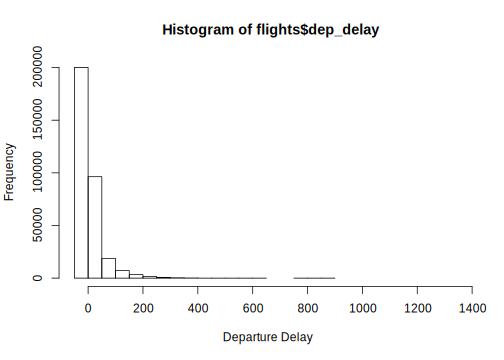
\includegraphics{mtec_cadi_2017_files/figure-latex/hist_delay-1.pdf}

The \texttt{nclass} parameter controls the number of bins into which the
\texttt{dep\_delay} range is divided. Try changing that parameter and
see what happens.

Now, we can (conceptually) make the bins as small as possible and get a
smooth curve that describes the \emph{distribution} of values of the
\texttt{dep\_delay} variable. We call this a \emph{density} plot:

\begin{Shaded}
\begin{Highlighting}[]
\KeywordTok{plot}\NormalTok{(}\KeywordTok{density}\NormalTok{(flights}\OperatorTok{$}\NormalTok{dep_delay, }\DataTypeTok{na.rm=}\OtherTok{TRUE}\NormalTok{), }\DataTypeTok{xlab=}\StringTok{"Departure Delay"}\NormalTok{)}
\end{Highlighting}
\end{Shaded}

\includegraphics{mtec_cadi_2017_files/figure-latex/density_delay-1.pdf}

Now, one more very useful way of succintly graphically summarizing the
distribution of a variable is using a \texttt{boxplot}.

\begin{Shaded}
\begin{Highlighting}[]
\KeywordTok{boxplot}\NormalTok{(flights}\OperatorTok{$}\NormalTok{dep_delay, }\DataTypeTok{ylab=}\StringTok{"Departure Delay"}\NormalTok{)}
\end{Highlighting}
\end{Shaded}

\includegraphics{mtec_cadi_2017_files/figure-latex/boxplot_delay-1.pdf}

That's not very clear to see, so let's do a transformation of this data
to see this better:

\begin{Shaded}
\begin{Highlighting}[]
\KeywordTok{boxplot}\NormalTok{(}\KeywordTok{log}\NormalTok{(flights}\OperatorTok{$}\NormalTok{dep_delay }\OperatorTok{-}\StringTok{ }
\StringTok{            }\KeywordTok{min}\NormalTok{(flights}\OperatorTok{$}\NormalTok{dep_delay,}\DataTypeTok{na.rm=}\OtherTok{TRUE}\NormalTok{)}
            \OperatorTok{+}\DecValTok{1}\NormalTok{), }\DataTypeTok{ylab=}\StringTok{"Departure Delay"}\NormalTok{)}
\end{Highlighting}
\end{Shaded}

\includegraphics{mtec_cadi_2017_files/figure-latex/boxplot_transformed_delay-1.pdf}

So what does this represent: (a) central tendency (using the median) is
represented by the black line within the box, (b) spread (using
inter-quartile range) is represented by the box and whiskers. (c)
outliers (data that is \emph{unusually} outside the spread of the data)

We will see more formal descriptions of these summary statistics in the
next section, but you can see what we are trying to capture with them
graphically.

\subsection{Visualization of pairs of
variables}\label{visualization-of-pairs-of-variables}

Now we can start looking at the relationship between pairs of variables.
Suppose we want to see the relationship between \texttt{dep\_delay}, a
\emph{numeric} variable, and \texttt{origin}, a \emph{categorical}
variable. The neat thing here is that we can start thinking about
conditioning as we saw before. Here is how we can see a plot of the
distribution of departure delays \emph{conditioned} on origin airport.

\begin{Shaded}
\begin{Highlighting}[]
\KeywordTok{boxplot}\NormalTok{(}\KeywordTok{log}\NormalTok{(flights}\OperatorTok{$}\NormalTok{dep_delay }\OperatorTok{-}\StringTok{ }\KeywordTok{min}\NormalTok{(flights}\OperatorTok{$}\NormalTok{dep_delay, }\DataTypeTok{na.rm=}\OtherTok{TRUE}\NormalTok{) }\OperatorTok{+}\StringTok{ }\DecValTok{1}\NormalTok{) }\OperatorTok{~}\StringTok{ }\NormalTok{flights}\OperatorTok{$}\NormalTok{origin,}
        \DataTypeTok{ylab=}\StringTok{"Departure Delay"}\NormalTok{, }\DataTypeTok{xlab=}\StringTok{"Airport of origin"}\NormalTok{)}
\end{Highlighting}
\end{Shaded}

\includegraphics{mtec_cadi_2017_files/figure-latex/delay_by_origin-1.pdf}

For pairs of continuous variables, the most useful visualization is the
scatter plot. This gives an idea of how one variable varies conditioned
on another variable.

\begin{Shaded}
\begin{Highlighting}[]
\KeywordTok{plot}\NormalTok{(flights}\OperatorTok{$}\NormalTok{dep_delay, flights}\OperatorTok{$}\NormalTok{arr_delay, }\DataTypeTok{xlab=}\StringTok{"Departure Delay"}\NormalTok{, }\DataTypeTok{ylab=}\StringTok{"Arrival Delay"}\NormalTok{)}
\end{Highlighting}
\end{Shaded}

\includegraphics{mtec_cadi_2017_files/figure-latex/delay_scatter-1.pdf}

\section{EDA with the grammar of
graphics}\label{eda-with-the-grammar-of-graphics}

While we have seen a basic repertoire of graphics it's easier to proceed
if we have a bit more formal way of thinking about graphics and plots.
Here is where we will use the \emph{grammar of graphics} implemented in
R by the package \texttt{ggplot2}.

The central premise is to characterize the building pieces behind plots:

\begin{enumerate}
\def\labelenumi{\arabic{enumi}.}
\tightlist
\item
  The data that goes into a plot, works best when data is tidy
\item
  The mapping between data and \emph{aesthetic} attributes
\item
  The \emph{geometric} representation of these attributes
\end{enumerate}

Let's start with a simple example:

\begin{Shaded}
\begin{Highlighting}[]
\KeywordTok{library}\NormalTok{(dplyr)}
\KeywordTok{library}\NormalTok{(ggplot2)}
\KeywordTok{library}\NormalTok{(Lahman)}
\NormalTok{batting <-}\StringTok{ }\KeywordTok{tbl_df}\NormalTok{(Batting)}

\CommentTok{# scatter plot of at bats vs. runs for 2010}
\NormalTok{batting }\OperatorTok\StringTok{ }
\StringTok{  }\KeywordTok{filter}\NormalTok{(yearID }\OperatorTok{==}\StringTok{ "2010"}\NormalTok{) }\OperatorTok
\StringTok{  }\KeywordTok{ggplot}\NormalTok{(}\KeywordTok{aes}\NormalTok{(}\DataTypeTok{x=}\NormalTok{AB, }\DataTypeTok{y=}\NormalTok{R)) }\OperatorTok{+}
\StringTok{    }\KeywordTok{geom_point}\NormalTok{()}
\end{Highlighting}
\end{Shaded}

\includegraphics{mtec_cadi_2017_files/figure-latex/unnamed-chunk-95-1.pdf}

\textbf{Data}: Batting table filtering for year\\
\textbf{Aesthetic attributes}: - x-axis mapped to variables \texttt{AB}
- y-axis mapped to variable \texttt{R}

\textbf{Geometric Representation}: points!

Now, you can cleanly distinguish the constituent parts of the plot.
E.g., change the geometric representation

\begin{Shaded}
\begin{Highlighting}[]
\CommentTok{# scatter plot of at bats vs. runs for 2010}
\NormalTok{batting }\OperatorTok\StringTok{ }
\StringTok{  }\KeywordTok{filter}\NormalTok{(yearID }\OperatorTok{==}\StringTok{ "2010"}\NormalTok{) }\OperatorTok
\StringTok{  }\KeywordTok{ggplot}\NormalTok{(}\KeywordTok{aes}\NormalTok{(}\DataTypeTok{x=}\NormalTok{AB, }\DataTypeTok{y=}\NormalTok{R, }\DataTypeTok{label=}\NormalTok{teamID)) }\OperatorTok{+}
\StringTok{    }\KeywordTok{geom_text}\NormalTok{() }\OperatorTok{+}
\StringTok{    }\KeywordTok{geom_point}\NormalTok{()}
\end{Highlighting}
\end{Shaded}

\includegraphics{mtec_cadi_2017_files/figure-latex/unnamed-chunk-96-1.pdf}

E.g., change the data.

\begin{Shaded}
\begin{Highlighting}[]
\CommentTok{# scatter plot of at bats vs. runs for 1995}
\NormalTok{batting }\OperatorTok\StringTok{ }
\StringTok{  }\KeywordTok{filter}\NormalTok{(yearID }\OperatorTok{==}\StringTok{ "1995"}\NormalTok{) }\OperatorTok
\StringTok{  }\KeywordTok{ggplot}\NormalTok{(}\KeywordTok{aes}\NormalTok{(}\DataTypeTok{x=}\NormalTok{AB, }\DataTypeTok{y=}\NormalTok{R)) }\OperatorTok{+}
\StringTok{    }\KeywordTok{geom_point}\NormalTok{()}
\end{Highlighting}
\end{Shaded}

\includegraphics{mtec_cadi_2017_files/figure-latex/unnamed-chunk-97-1.pdf}

E.g., change the aesthetic.

\begin{Shaded}
\begin{Highlighting}[]
\CommentTok{# scatter plot of at bats vs. hits for 2010}
\NormalTok{batting }\OperatorTok\StringTok{ }
\StringTok{  }\KeywordTok{filter}\NormalTok{(yearID }\OperatorTok{==}\StringTok{ "2010"}\NormalTok{) }\OperatorTok
\StringTok{  }\KeywordTok{ggplot}\NormalTok{(}\KeywordTok{aes}\NormalTok{(}\DataTypeTok{x=}\NormalTok{AB, }\DataTypeTok{y=}\NormalTok{H)) }\OperatorTok{+}
\StringTok{    }\KeywordTok{geom_point}\NormalTok{()}
\end{Highlighting}
\end{Shaded}

\includegraphics{mtec_cadi_2017_files/figure-latex/unnamed-chunk-98-1.pdf}

Let's make a line plot

What do we change? (data, aesthetic or geometry?)

\begin{Shaded}
\begin{Highlighting}[]
\NormalTok{batting }\OperatorTok
\StringTok{  }\KeywordTok{filter}\NormalTok{(yearID }\OperatorTok{==}\StringTok{ "2010"}\NormalTok{) }\OperatorTok
\StringTok{  }\KeywordTok{sample_n}\NormalTok{(}\DecValTok{100}\NormalTok{) }\OperatorTok
\StringTok{  }\KeywordTok{ggplot}\NormalTok{(}\KeywordTok{aes}\NormalTok{(}\DataTypeTok{x=}\NormalTok{AB, }\DataTypeTok{y=}\NormalTok{H)) }\OperatorTok{+}
\StringTok{  }\KeywordTok{geom_line}\NormalTok{()}
\end{Highlighting}
\end{Shaded}

\includegraphics{mtec_cadi_2017_files/figure-latex/unnamed-chunk-99-1.pdf}

Let's add a regression line

What do we add? (data, aesthetic or geometry?)

\begin{Shaded}
\begin{Highlighting}[]
\NormalTok{batting }\OperatorTok
\StringTok{  }\KeywordTok{filter}\NormalTok{(yearID }\OperatorTok{==}\StringTok{ "2010"}\NormalTok{) }\OperatorTok
\StringTok{  }\KeywordTok{ggplot}\NormalTok{(}\KeywordTok{aes}\NormalTok{(}\DataTypeTok{x=}\NormalTok{AB, }\DataTypeTok{y=}\NormalTok{H)) }\OperatorTok{+}
\StringTok{  }\KeywordTok{geom_point}\NormalTok{() }\OperatorTok{+}\StringTok{ }
\StringTok{  }\KeywordTok{geom_smooth}\NormalTok{(}\DataTypeTok{method=}\NormalTok{lm)}
\end{Highlighting}
\end{Shaded}

\includegraphics{mtec_cadi_2017_files/figure-latex/unnamed-chunk-100-1.pdf}

\subsection{Other aesthetics}\label{other-aesthetics}

Using other aesthetics we can incorporate information from other
variables.

Color: color by categorical variable

\begin{Shaded}
\begin{Highlighting}[]
\NormalTok{batting }\OperatorTok
\StringTok{  }\KeywordTok{filter}\NormalTok{(yearID }\OperatorTok{==}\StringTok{ "2010"}\NormalTok{) }\OperatorTok
\StringTok{  }\KeywordTok{ggplot}\NormalTok{(}\KeywordTok{aes}\NormalTok{(}\DataTypeTok{x=}\NormalTok{AB, }\DataTypeTok{y=}\NormalTok{H, }\DataTypeTok{color=}\NormalTok{lgID)) }\OperatorTok{+}
\StringTok{  }\KeywordTok{geom_point}\NormalTok{() }\OperatorTok{+}\StringTok{ }
\StringTok{  }\KeywordTok{geom_smooth}\NormalTok{(}\DataTypeTok{method=}\NormalTok{lm)}
\end{Highlighting}
\end{Shaded}

\includegraphics{mtec_cadi_2017_files/figure-latex/unnamed-chunk-101-1.pdf}

Size: size by (discrete) numeric variable

\begin{Shaded}
\begin{Highlighting}[]
\NormalTok{batting }\OperatorTok
\StringTok{  }\KeywordTok{filter}\NormalTok{(yearID }\OperatorTok{==}\StringTok{ "2010"}\NormalTok{) }\OperatorTok
\StringTok{  }\KeywordTok{ggplot}\NormalTok{(}\KeywordTok{aes}\NormalTok{(}\DataTypeTok{x=}\NormalTok{AB, }\DataTypeTok{y=}\NormalTok{R, }\DataTypeTok{size=}\NormalTok{HR)) }\OperatorTok{+}
\StringTok{  }\KeywordTok{geom_point}\NormalTok{() }\OperatorTok{+}\StringTok{ }
\StringTok{  }\KeywordTok{geom_smooth}\NormalTok{(}\DataTypeTok{method=}\NormalTok{lm)}
\end{Highlighting}
\end{Shaded}

\includegraphics{mtec_cadi_2017_files/figure-latex/unnamed-chunk-102-1.pdf}

\subsection{Faceting}\label{faceting}

The last major component of exploratory analysis called
\texttt{faceting} in visualization, corresponds to \texttt{conditioning}
in statistical modeling, we've seen it as the motivation of
\texttt{grouping} when wrangling data.

\begin{Shaded}
\begin{Highlighting}[]
\NormalTok{batting }\OperatorTok
\StringTok{  }\KeywordTok{filter}\NormalTok{(yearID }\OperatorTok\StringTok{ }\KeywordTok{c}\NormalTok{(}\StringTok{"1995"}\NormalTok{, }\StringTok{"2000"}\NormalTok{, }\StringTok{"2010"}\NormalTok{)) }\OperatorTok
\StringTok{  }\KeywordTok{ggplot}\NormalTok{(}\KeywordTok{aes}\NormalTok{(}\DataTypeTok{x=}\NormalTok{AB, }\DataTypeTok{y=}\NormalTok{R, }\DataTypeTok{size=}\NormalTok{HR)) }\OperatorTok{+}
\StringTok{  }\KeywordTok{facet_grid}\NormalTok{(lgID}\OperatorTok{~}\NormalTok{yearID) }\OperatorTok{+}
\StringTok{  }\KeywordTok{geom_point}\NormalTok{() }\OperatorTok{+}\StringTok{ }
\StringTok{  }\KeywordTok{geom_smooth}\NormalTok{(}\DataTypeTok{method=}\NormalTok{lm)}
\end{Highlighting}
\end{Shaded}

\includegraphics{mtec_cadi_2017_files/figure-latex/unnamed-chunk-103-1.pdf}

\section{Exercise}\label{exercise-1}

Use \texttt{ggplot2} to make a scatter plot of domestic gross revenue
vs.~Rotten Tomato rating for Diego Luna's movies.

\chapter{Capstone Project 1}\label{capstone-project-1}

\section{Project 1}\label{project-1}

\begin{itemize}
\item
  Write a script that includes all steps for scraping, cleaning,
  manipulating and making the Diego Luna movie analysis plot.
\item
  Write a set of functions to perform the same analysis given an actor's
  name
\end{itemize}

\section{Project 2}\label{project-2}

Download data from the ENADID and make a plot of internal vs.~external
migration patterns in Mexico from 1992 to 2014. Data for 2009 can be
found here:
\url{http://www.beta.inegi.org.mx/proyectos/enchogares/especiales/enadid/2009/default.html}.
Data for other years is also available there. Write your analysis in an
R script.

\chapter{Introduction to tidy regression
analysis}\label{introduction-to-tidy-regression-analysis}

Linear regression is a very elegant, simple, powerful and commonly used
technique for data analysis.

\section{Simple Regression}\label{simple-regression}

Let's start with the simplest linear model. The goal here is to analyze
the relationship between a \emph{continuous numerical} variable \(Y\)
and another (\emph{numerical} or \emph{categorical}) variable \(X\). We
assume that in our population of interest the relationship between the
two is given by a linear function:

\[
Y = \beta_0 + \beta_1 X
\]

Here is (simulated) data from an advertising campaign measuring sales
and the amount spent in advertising. We think that sales are related to
the amount of money spent on TV advertising:

\[
\mathtt{sales} \approx \beta_0 + \beta_1 \times \mathtt{TV}
\]

\begin{figure}
\centering
\includegraphics{img/regression_example.png}
\caption{}
\end{figure}

Given this data, we would say that we \emph{regress} \texttt{sales} on
\texttt{TV} when we perform this regression analysis. As before, given
data we would like to estimate what this relationship is in the
\emph{population} (what is the population in this case?). What do we
need to estimate in this case? Values for \(\beta_0\) and \(\beta_1\).

Let's take a look at some data. Here is data measuring characteristics
of cars, including horsepower, weight, displacement, miles per gallon.
Let's see how well a linear model captures the relationship between
miles per gallon and weight

\begin{Shaded}
\begin{Highlighting}[]
\KeywordTok{library}\NormalTok{(ISLR)}
\KeywordTok{library}\NormalTok{(dplyr)}
\KeywordTok{library}\NormalTok{(ggplot2)}
\KeywordTok{library}\NormalTok{(broom)}

\KeywordTok{data}\NormalTok{(Auto)}

\NormalTok{Auto }\OperatorTok
\StringTok{  }\KeywordTok{ggplot}\NormalTok{(}\KeywordTok{aes}\NormalTok{(}\DataTypeTok{x=}\NormalTok{weight, }\DataTypeTok{y=}\NormalTok{mpg)) }\OperatorTok{+}
\StringTok{    }\KeywordTok{geom_point}\NormalTok{() }\OperatorTok{+}\StringTok{ }
\StringTok{    }\KeywordTok{geom_smooth}\NormalTok{(}\DataTypeTok{method=}\NormalTok{lm) }\OperatorTok{+}\StringTok{ }
\StringTok{    }\KeywordTok{theme_minimal}\NormalTok{()}
\end{Highlighting}
\end{Shaded}

\includegraphics{mtec_cadi_2017_files/figure-latex/unnamed-chunk-104-1.pdf}

In R, linear models are built using the \texttt{lm} function

\begin{Shaded}
\begin{Highlighting}[]
\NormalTok{auto_fit <-}\StringTok{ }\KeywordTok{lm}\NormalTok{(mpg}\OperatorTok{~}\NormalTok{weight, }\DataTypeTok{data=}\NormalTok{Auto)}
\NormalTok{auto_fit}
\end{Highlighting}
\end{Shaded}

\begin{verbatim}
## 
## Call:
## lm(formula = mpg ~ weight, data = Auto)
## 
## Coefficients:
## (Intercept)       weight  
##   46.216525    -0.007647
\end{verbatim}

This states that for this dataset \(\hat{\beta}_0 = 46.2165245\) and
\(\hat{\beta}_1 = -0.0076473\). What's the interpretation? According to
this model, a weightless car \texttt{weight=0} would run
\(\approx 46.22\) \emph{miles per gallon} on average, and, on average, a
car would run \(\approx 0.008\) \emph{miles per gallon} fewer for every
extra \emph{pound} of weight. Note, that the units of the outcome \(Y\)
and the predictor \(X\) matter for the interpretation of these values.

\section{Inference}\label{inference}

Now that we have an estimate, we want to know how good of an estimate
this is. An important point to understand is that like the sample mean,
the regression line we learn from a specific dataset is an estimate. A
different sample from the same population would give us a different
estimate (regression line).

But, statistical theory tells us that, on average, we are close to
population regression line (I.e., close to \(\beta_0\) and \(\beta_1\)),
that the spread around \(\beta_0\) and \(\beta_1\) is well approximated
by a normal distribution and that the spread goes to zero as the sample
size increases.

\begin{figure}
\centering
\includegraphics{img/population_line.png}
\caption{}
\end{figure}

\subsection{Confidence Interval}\label{confidence-interval}

We can construct a confidence interval to say how precise we think our
estimates of the population regression line is. In particular, we want
to see how precise our estimate of \(\beta_1\) is, since that captures
the relationship between the two variables.

\begin{Shaded}
\begin{Highlighting}[]
\NormalTok{auto_fit_stats <-}\StringTok{ }\NormalTok{auto_fit }\OperatorTok
\StringTok{  }\KeywordTok{tidy}\NormalTok{() }\OperatorTok
\StringTok{  }\KeywordTok{select}\NormalTok{(term, estimate, std.error)}
\NormalTok{auto_fit_stats}
\end{Highlighting}
\end{Shaded}

\begin{verbatim}
##          term     estimate    std.error
## 1 (Intercept) 46.216524549 0.7986724633
## 2      weight -0.007647343 0.0002579633
\end{verbatim}

This \texttt{tidy} function is defined by the \texttt{broom} package,
which is very handy to manipulate the result of learning models in a
consistent manner. The \texttt{select} call removes some extra
information that we will discuss shortly.

Given the confidence interval, we would say, ``on average, a car runs
\(_{-0.0082} -0.0076_{-0.0071}\) \emph{miles per gallon} fewer per pound
of weight.

\subsection{\texorpdfstring{The \(t\)-statistic and the
\(t\)-distribution}{The t-statistic and the t-distribution}}\label{the-t-statistic-and-the-t-distribution}

We can also test a null hypothesis about this relationship: ``there is
no relationship between weight and miles per gallon'', which translates
to \(\beta_1=0\). According to the statistical theory if this hypothesis
is true then the distribution of \(\hat{\beta}_1\) is well approximated
by \(N(0,\mathrm{se}(\hat{\beta}_1))\), and if we observe the estimated
\(\hat{\beta}_1\) is \emph{too far} from 0 according to this
distribution then we \emph{reject} the hypothesis.

Now, there is a technicality here that is worth paying attention to. The
normal approximation is good as sample size increases, but what about
moderate sample sizes (say, less than 100)? The \(t\) distribution
provides a better approximation of the sampling distribution of these
estimates for moderate sample sizes, and it tends to the normal
distribution as sample size increases.

The \(t\) distribution is commonly used in this testing situation to
obtain the probability of rejecting the null hypothesis. It is based on
the \(t\)-statistic

\[
\frac{\hat{\beta}_1}{\mathrm{se}(\hat{\beta}_1)}
\]

You can think of this as a \emph{signal-to-noise} ratio, or a
standardizing transformation on the estimated parameter. Under the null
hypothesis, it was shown that the \(t\)-statistic is well approximated
by a \(t\)-distribution with \(n-2\) \emph{degrees of freedom} (we will
get back to \emph{degrees of freedom} shortly).

In our example, we get a \(t\) statistic and P-value as follows:

\begin{Shaded}
\begin{Highlighting}[]
\NormalTok{auto_fit_stats <-}\StringTok{ }\NormalTok{auto_fit }\OperatorTok
\StringTok{  }\KeywordTok{tidy}\NormalTok{()}
\NormalTok{auto_fit_stats}
\end{Highlighting}
\end{Shaded}

\begin{verbatim}
##          term     estimate    std.error statistic       p.value
## 1 (Intercept) 46.216524549 0.7986724633  57.86668 1.623069e-193
## 2      weight -0.007647343 0.0002579633 -29.64508 6.015296e-102
\end{verbatim}

We would say: ``We found a statistically significant relationship
between weight and miles per gallon. On average, a car runs
\(_{-0.0082} -0.0076_{-0.0071}\) \emph{miles per gallon} fewer per pound
of weight (\(t\)=-29.65, \(p\)-value \textless{}
\(6.02\times 10^{-102}\)).''

\subsection{Global Fit}\label{global-fit}

Now, notice that we can make \emph{predictions} based on our regression
model, and that prediction should be better than a prediction with a
simple average. We can use this comparison as a measure of how good of a
job we are doing using our model to fit this data: how much of the
variance of \(Y\) can we \emph{explain} with our model. To do this we
can calculate \emph{total sum of squares}:

\[
TSS = \sum_i (y_i - \overline{y})^2
\]

(this is the squared error of a prediction using the sample mean of
\(Y\))

and the \emph{residual sum of squares}:

\[
RSS = \sum_i (y_i - \hat{y}_i)^2
\]

(which is the squared error of a prediction using the linear model we
learned)

The commonly used \(R^2\) measure comparse these two quantities:

\[
R^2 = \frac{\mathrm{TSS}-\mathrm{RSS}}{\mathrm{TSS}} = 1 - \frac{\mathrm{RSS}}{\mathrm{TSS}}
\]

These types of global statistics for the linear model can be obtained
using the \texttt{glance} function in the \texttt{broom} package. In our
example

\begin{Shaded}
\begin{Highlighting}[]
\NormalTok{auto_fit }\OperatorTok
\StringTok{  }\KeywordTok{glance}\NormalTok{() }\OperatorTok
\StringTok{  }\KeywordTok{select}\NormalTok{(r.squared, sigma, statistic, df, p.value)}
\end{Highlighting}
\end{Shaded}

\begin{verbatim}
##   r.squared    sigma statistic df       p.value
## 1 0.6926304 4.332712  878.8309  2 6.015296e-102
\end{verbatim}

We will explain the the columns \texttt{statistic}, \texttt{df} and
\texttt{p.value} when we discuss regression using more than a single
predictor \(X\).

\section{Some important
technicalities}\label{some-important-technicalities}

We mentioned above that predictor \(X\) could be \emph{numeric} or
\emph{categorical}. However, this is not precisely true. We can use a
transformation to represent \emph{categorical} variables. Here is a
simple example:

Suppose we have a categorical variable \texttt{sex} with values
\texttt{female} and \texttt{male}, and we want to show the relationship
between, say \texttt{credit\ card\ balance} and \texttt{sex}. We can
create a dummy variable \(x\) as follows:

\[
x_i = \left\{
\begin{aligned}
1 & \textrm{ if female} \\
0 & \textrm{o.w.}
\end{aligned}
\right.
\]

and fit a model \(y = \beta_0 + \beta_1 x\). What is the conditional
expectation given by this model? If the person is male, then
\(y=\beta_0\), if the person is female, then \(y=\beta_0 + \beta_1\).
So, what is the interpretation of \(\beta_1\)? The average difference in
credit card balance between females and males.

We could do a different encoding:

\[
x_i = \left\{
\begin{aligned}
+1 & \textrm{ if female} \\
-1 & \textrm{o.w.}
\end{aligned}
\right.
\]

Then what is the interpretation of \(\beta_1\) in this case?

Note, that when we call the \texttt{lm(y\textasciitilde{}x)} function
and \texttt{x} is a factor with two levels, the first transformation is
used by default. What if there are more than 2 levels? We need multiple
regression, which we will see shortly.

\section{Issues with linear
regression}\label{issues-with-linear-regression}

There are some assumptions underlying the inferences and predictions we
make using linear regression that we should verify are met when we use
this framework. Let's start with four important ones that apply to
simple regression

\subsection{Non-linearity of outcome-predictor
relationship}\label{non-linearity-of-outcome-predictor-relationship}

What if the underlying relationship is not linear? We will see later
that we can capture non-linear relationships between variables, but for
now, let's concentrate on detecting if a linear relationship is a good
approximation. We can use exploratory visual analysis to do this for now
by plotting residuals \((y_i - \hat{y}_i)^2\) as a function of the
fitted values \(\hat{y}_i\).

The \texttt{broom} package uses the \texttt{augment} function to help
with this task. It augments the input data used to learn the linear
model with information of the fitted model for each observation

\begin{Shaded}
\begin{Highlighting}[]
\NormalTok{augmented_auto <-}\StringTok{ }\NormalTok{auto_fit }\OperatorTok
\StringTok{  }\KeywordTok{augment}\NormalTok{()}
\NormalTok{augmented_auto }\OperatorTok\StringTok{ }\KeywordTok{head}\NormalTok{()}
\end{Highlighting}
\end{Shaded}

\begin{verbatim}
##   .rownames mpg weight  .fitted   .se.fit    .resid        .hat   .sigma
## 1         1  18   3504 19.42024 0.2575448 -1.420236 0.003533343 4.337678
## 2         2  15   3693 17.97489 0.2862653 -2.974889 0.004365337 4.335643
## 3         3  18   3436 19.94026 0.2487426 -1.940256 0.003295950 4.337158
## 4         4  16   3433 19.96320 0.2483756 -3.963198 0.003286232 4.333606
## 5         5  17   3449 19.84084 0.2503543 -2.840840 0.003338799 4.335878
## 6         6  15   4341 13.01941 0.4142337  1.980589 0.009140525 4.337104
##        .cooksd .std.resid
## 1 0.0001911753 -0.3283745
## 2 0.0010380292 -0.6881147
## 3 0.0003326721 -0.4485553
## 4 0.0013838821 -0.9162219
## 5 0.0007225022 -0.6567698
## 6 0.0009727164  0.4592282
\end{verbatim}

With that we can make the plot we need to check for possible
non-linearity

\begin{Shaded}
\begin{Highlighting}[]
\NormalTok{augmented_auto }\OperatorTok
\StringTok{  }\KeywordTok{ggplot}\NormalTok{(}\KeywordTok{aes}\NormalTok{(}\DataTypeTok{x=}\NormalTok{.fitted,}\DataTypeTok{y=}\NormalTok{.resid)) }\OperatorTok{+}
\StringTok{    }\KeywordTok{geom_point}\NormalTok{() }\OperatorTok{+}\StringTok{ }
\StringTok{    }\KeywordTok{geom_smooth}\NormalTok{() }\OperatorTok{+}
\StringTok{    }\KeywordTok{labs}\NormalTok{(}\DataTypeTok{x=}\StringTok{"fitted"}\NormalTok{, }\DataTypeTok{y=}\StringTok{"residual"}\NormalTok{)}
\end{Highlighting}
\end{Shaded}

\begin{verbatim}
## `geom_smooth()` using method = 'loess'
\end{verbatim}

\includegraphics{mtec_cadi_2017_files/figure-latex/unnamed-chunk-111-1.pdf}

\subsection{Correlated Error}\label{correlated-error}

For our inferences to be valid, we need residuals to be independent and
identically distributed. We can spot non independence if we observe a
trend in residuals as a function of the predictor \(X\). Here is a
simulation to demonstrate this:

\begin{figure}
\centering
\includegraphics{img/correlated_error.png}
\caption{}
\end{figure}

In this case, our standard error estimates would be underestimated and
our confidence intervals and hypothesis testing results would be biased.

\subsection{Non-constant variance}\label{non-constant-variance}

Another violation of the iid assumption would be observed if the spread
of residuals is not independent of the fitted values. Here is an
illustration, and a possible fix using a log transformation on the
outcome \(Y\).

\begin{figure}
\centering
\includegraphics{img/residual_variance.png}
\caption{}
\end{figure}

\section{Multivariate Regression}\label{multivariate-regression}

Now that we've seen regression using a single predictor we'll move on to
regression using multiple predictors. In this case, we use models of
conditional expectation represented as linear functions of multiple
variables.

In the case of our advertising example, this would be a model:

\[
\mathtt{sales} = \beta_0 + \beta_1 \times \mathtt{TV} + \beta_2 \times \mathtt{newspaper} + \beta_3 \times \mathtt{facebook}
\]

These models let us make statements of the type: ``holding everything
else constant, sales increased on average by 1000 per dollar spent on
Facebook advertising'' (this would be given by parameter \(\beta_3\) in
the example model).

\subsection{Estimation in multivariate
regression}\label{estimation-in-multivariate-regression}

Continuing with our Auto example, we can build a model for miles per
gallon using multiple predictors:

\begin{Shaded}
\begin{Highlighting}[]
\NormalTok{auto_fit <-}\StringTok{ }\KeywordTok{lm}\NormalTok{(mpg}\OperatorTok{~}\DecValTok{1}\OperatorTok{+}\NormalTok{weight}\OperatorTok{+}\NormalTok{cylinders}\OperatorTok{+}\NormalTok{horsepower}\OperatorTok{+}\NormalTok{displacement}\OperatorTok{+}\NormalTok{year, }\DataTypeTok{data=}\NormalTok{Auto)}
\NormalTok{auto_fit}
\end{Highlighting}
\end{Shaded}

\begin{verbatim}
## 
## Call:
## lm(formula = mpg ~ 1 + weight + cylinders + horsepower + displacement + 
##     year, data = Auto)
## 
## Coefficients:
##  (Intercept)        weight     cylinders    horsepower  displacement  
##   -12.779493     -0.006524     -0.343690     -0.007715      0.006996  
##         year  
##     0.749924
\end{verbatim}

From this model we can make the statement: ``Holding everything else
constant, cars run 0.76 miles per gallon more each year on average''.

\subsection{Statistical statements
(cont'd)}\label{statistical-statements-contd}

Like simple linear regression, we can construct confidence intervals,
and test a null hypothesis of no relationship (\(\beta_j=0\)) for the
parameter corresponding to each predictor. This is again nicely managed
by the \texttt{broom} package:

\begin{Shaded}
\begin{Highlighting}[]
\NormalTok{auto_fit_stats <-}\StringTok{ }\NormalTok{auto_fit }\OperatorTok
\StringTok{  }\KeywordTok{tidy}\NormalTok{()}
\NormalTok{auto_fit_stats }\OperatorTok\StringTok{ }\NormalTok{knitr}\OperatorTok{::}\KeywordTok{kable}\NormalTok{()}
\end{Highlighting}
\end{Shaded}

\begin{tabular}{l|r|r|r|r}
\hline
term & estimate & std.error & statistic & p.value\\
\hline
(Intercept) & -12.7794934 & 4.2739387 & -2.9900975 & 0.0029676\\
\hline
weight & -0.0065245 & 0.0005866 & -11.1215621 & 0.0000000\\
\hline
cylinders & -0.3436900 & 0.3315619 & -1.0365786 & 0.3005812\\
\hline
horsepower & -0.0077149 & 0.0107036 & -0.7207702 & 0.4714872\\
\hline
displacement & 0.0069964 & 0.0073095 & 0.9571736 & 0.3390787\\
\hline
year & 0.7499243 & 0.0524361 & 14.3016700 & 0.0000000\\
\hline
\end{tabular}

In this case we would reject the null hypothesis of no relationship only
for predictors \texttt{weight} and \texttt{year}. We would write the
statement for year as follows:

``Holding everything else constant, cars run \({}_{0.65} 0.75_{0.85}\)
miles per gallon more each year on average (P-value\(<1e-16\))''.

\subsection{The F-test}\label{the-f-test}

We can make additional statements for multivariate regression: ``is
there a relationship between \emph{any} of the predictors and the
response?''. Mathematically, we write this as
\(\beta_1 = \beta_2 = \cdots = \beta_p = 0\).

Under the null, our model for \(y\) would be estimated by the sample
mean \(\overline{y}\), and the error for that estimate is by total sum
of squared error \(TSS\). As before, we can compare this to the residual
sum of squared error \(RSS\) using the \(F\) statistic:

\[
\frac{(\mathrm{TSS}-\mathrm{RSS})/p}{\mathrm{RSS}/(n-p-1)}
\]

If this statistic is greater (enough) than 1, then we reject hypothesis
that there is no relationship between response and predictors.

Back to our example, we use the \texttt{glance} function to compute this
type of summary:

\begin{Shaded}
\begin{Highlighting}[]
\NormalTok{auto_fit }\OperatorTok\StringTok{ }
\StringTok{  }\KeywordTok{glance}\NormalTok{() }\OperatorTok
\StringTok{  }\KeywordTok{select}\NormalTok{(r.squared, sigma, statistic, df, p.value) }\OperatorTok
\StringTok{  }\NormalTok{knitr}\OperatorTok{::}\KeywordTok{kable}\NormalTok{()}
\end{Highlighting}
\end{Shaded}

\begin{tabular}{r|r|r|r|r}
\hline
r.squared & sigma & statistic & df & p.value\\
\hline
0.8089093 & 3.433902 & 326.7965 & 6 & 0\\
\hline
\end{tabular}

In comparison with the linear model only using \texttt{weight}, this
multivariate model explains \emph{more of the variance} of \texttt{mpg},
but using more predictors. This is where the notion of \emph{degrees of
freedom} comes in: we now have a model with expanded
\emph{representational} ability.

However, the bigger the model, we are conditioning more and more, and
intuitively, given a fixed dataset, have fewer data points to estimate
conditional expectation for each value of the predictors. That means,
that are estimated conditional expectation is less \emph{precise}.

To capture this phenomenon, we want statistics that tradeoff how well
the model fits the data, and the ``complexity'' of the model. Now, we
can look at the full output of the \texttt{glance} function:

\begin{Shaded}
\begin{Highlighting}[]
\NormalTok{auto_fit }\OperatorTok
\StringTok{  }\KeywordTok{glance}\NormalTok{() }\OperatorTok
\StringTok{  }\NormalTok{knitr}\OperatorTok{::}\KeywordTok{kable}\NormalTok{()}
\end{Highlighting}
\end{Shaded}

\begin{tabular}{r|r|r|r|r|r|r|r|r|r|r}
\hline
r.squared & adj.r.squared & sigma & statistic & p.value & df & logLik & AIC & BIC & deviance & df.residual\\
\hline
0.8089093 & 0.806434 & 3.433902 & 326.7965 & 0 & 6 & -1036.81 & 2087.62 & 2115.419 & 4551.589 & 386\\
\hline
\end{tabular}

Columns \texttt{AIC} and \texttt{BIC} display statistics that penalize
model fit with model size. The smaller this value, the better. Let's now
compare a model only using \texttt{weight}, a model only using
\texttt{weight} and \texttt{year} and the full multiple regression model
we saw before.

\begin{Shaded}
\begin{Highlighting}[]
\KeywordTok{lm}\NormalTok{(mpg}\OperatorTok{~}\NormalTok{weight, }\DataTypeTok{data=}\NormalTok{Auto) }\OperatorTok
\StringTok{  }\KeywordTok{glance}\NormalTok{() }\OperatorTok
\StringTok{  }\NormalTok{knitr}\OperatorTok{::}\KeywordTok{kable}\NormalTok{()}
\end{Highlighting}
\end{Shaded}

\begin{tabular}{r|r|r|r|r|r|r|r|r|r|r}
\hline
r.squared & adj.r.squared & sigma & statistic & p.value & df & logLik & AIC & BIC & deviance & df.residual\\
\hline
0.6926304 & 0.6918423 & 4.332712 & 878.8309 & 0 & 2 & -1129.969 & 2265.939 & 2277.852 & 7321.234 & 390\\
\hline
\end{tabular}

\begin{Shaded}
\begin{Highlighting}[]
\KeywordTok{lm}\NormalTok{(mpg}\OperatorTok{~}\NormalTok{weight}\OperatorTok{+}\NormalTok{year, }\DataTypeTok{data=}\NormalTok{Auto) }\OperatorTok
\StringTok{  }\KeywordTok{glance}\NormalTok{() }\OperatorTok
\StringTok{  }\NormalTok{knitr}\OperatorTok{::}\KeywordTok{kable}\NormalTok{()}
\end{Highlighting}
\end{Shaded}

\begin{tabular}{r|r|r|r|r|r|r|r|r|r|r}
\hline
r.squared & adj.r.squared & sigma & statistic & p.value & df & logLik & AIC & BIC & deviance & df.residual\\
\hline
0.8081803 & 0.8071941 & 3.427153 & 819.473 & 0 & 3 & -1037.556 & 2083.113 & 2098.998 & 4568.952 & 389\\
\hline
\end{tabular}

In this case, using more predictors beyond \texttt{weight} and
\texttt{year} doesn't help.

\subsection{Categorical predictors
(cont'd)}\label{categorical-predictors-contd}

We saw transformations for categorical predictors with only two values,
and deferred our discussion of categorical predictors with more than two
values. In our example we have the \texttt{origin} predictor,
corresponding to where the car was manufactured, which has multiple
values

\begin{Shaded}
\begin{Highlighting}[]
\NormalTok{Auto <-}\StringTok{ }\NormalTok{Auto }\OperatorTok
\StringTok{  }\KeywordTok{mutate}\NormalTok{(}\DataTypeTok{origin=}\KeywordTok{factor}\NormalTok{(origin))}
\KeywordTok{levels}\NormalTok{(Auto}\OperatorTok{$}\NormalTok{origin)}
\end{Highlighting}
\end{Shaded}

\begin{verbatim}
## [1] "1" "2" "3"
\end{verbatim}

As before, we can only use numerical predictors in linear regression
models. The most common way of doing this is to create new dummy
predictors to \emph{encode} the value of the categorical predictor.
Let's take a categorical variable \texttt{major} that can take values
\texttt{CS}, \texttt{MATH}, \texttt{BUS}. We can encode these values
using variables \(x_1\) and \(x_2\)

\[
x_1 = \left\{
\begin{aligned}
1 & \textrm{ if MATH} \\
0 & \textrm{ o.w.}
\end{aligned}
\right.
\]

\[
x_2 = \left\{
\begin{aligned}
1 & \textrm{ if BUS} \\
0 & \textrm{ o.w.}
\end{aligned}
\right.
\]

Now let's build a model to capture the relationship between
\texttt{salary} and \texttt{major}:

\[
\mathtt{salary} = \beta_0 + \beta_1 x_1 + \beta_2 x_2
\]

What is the expected salary for a CS major? \(\beta_0\).\\
For a MATH major? \(\beta_0 + \beta_1\). For a BUS major?
\(\beta_0 + \beta_2\).

So, \(\beta_1\) is the average difference in salary between MATH and CS
majors. How can we calculate the average difference in salary between
MATH and BUS majors? \(\beta_1 - \beta_2\).

The \texttt{lm} function in R does this transformation by default when a
variable has class \texttt{factor}. We can see what the underlying
numerical predictors look like by using the \texttt{model\_matrix}
function and passing it the model formula we build:

\begin{Shaded}
\begin{Highlighting}[]
\NormalTok{extended_df <-}\StringTok{ }\KeywordTok{model.matrix}\NormalTok{(}\OperatorTok{~}\KeywordTok{factor}\NormalTok{(origin), }\DataTypeTok{data=}\NormalTok{Auto) }\OperatorTok\StringTok{ }
\StringTok{  }\KeywordTok{as.data.frame}\NormalTok{() }\OperatorTok
\StringTok{  }\KeywordTok{mutate}\NormalTok{(}\DataTypeTok{origin =} \KeywordTok{factor}\NormalTok{(Auto}\OperatorTok{$}\NormalTok{origin))}
\end{Highlighting}
\end{Shaded}

\begin{Shaded}
\begin{Highlighting}[]
\NormalTok{extended_df }\OperatorTok
\StringTok{  }\KeywordTok{filter}\NormalTok{(origin }\OperatorTok{==}\StringTok{ "1"}\NormalTok{) }\OperatorTok\StringTok{ }\KeywordTok{head}\NormalTok{()}
\end{Highlighting}
\end{Shaded}

\begin{verbatim}
##   (Intercept) factor(origin)2 factor(origin)3 origin
## 1           1               0               0      1
## 2           1               0               0      1
## 3           1               0               0      1
## 4           1               0               0      1
## 5           1               0               0      1
## 6           1               0               0      1
\end{verbatim}

\begin{Shaded}
\begin{Highlighting}[]
\NormalTok{extended_df }\OperatorTok\StringTok{ }
\StringTok{  }\KeywordTok{filter}\NormalTok{(origin }\OperatorTok{==}\StringTok{ "2"}\NormalTok{) }\OperatorTok\StringTok{ }\KeywordTok{head}\NormalTok{()}
\end{Highlighting}
\end{Shaded}

\begin{verbatim}
##   (Intercept) factor(origin)2 factor(origin)3 origin
## 1           1               1               0      2
## 2           1               1               0      2
## 3           1               1               0      2
## 4           1               1               0      2
## 5           1               1               0      2
## 6           1               1               0      2
\end{verbatim}

\begin{Shaded}
\begin{Highlighting}[]
\NormalTok{extended_df }\OperatorTok
\StringTok{  }\KeywordTok{filter}\NormalTok{(origin }\OperatorTok{==}\StringTok{ "3"}\NormalTok{) }\OperatorTok\StringTok{ }\KeywordTok{head}\NormalTok{()}
\end{Highlighting}
\end{Shaded}

\begin{verbatim}
##   (Intercept) factor(origin)2 factor(origin)3 origin
## 1           1               0               1      3
## 2           1               0               1      3
## 3           1               0               1      3
## 4           1               0               1      3
## 5           1               0               1      3
## 6           1               0               1      3
\end{verbatim}

\section{Interactions in linear
models}\label{interactions-in-linear-models}

The linear models so far include \emph{additive} terms for a single
predictor. That let us made statemnts of the type ``holding everything
else constant\ldots{}''. But what if we think that a pair of predictors
\emph{together} have a relationship with the outcome. We can add these
\emph{interaction} terms to our linear models as products:

Consider the advertising example:

\[
  \mathtt{sales} = \beta_0 + \beta_1 \times \mathtt{TV} + \beta_2 \times \mathtt{facebook} + \beta_3 \times (\mathtt{TV} \times \mathtt{facebook})
\]

If \(\beta_3\) is positive, then the effect of increasing TV advertising
money is increased if facebook advertising is also increased.

When using categorical variables, interactions have an elegant
interpretation. Consider our car example, and suppose we build a model
with an interaction between \texttt{weight} and \texttt{origin}. Let's
look at what the numerical predictors look like:

\begin{Shaded}
\begin{Highlighting}[]
\NormalTok{Auto}\OperatorTok{$}\NormalTok{origin <-}\StringTok{ }\KeywordTok{factor}\NormalTok{(Auto}\OperatorTok{$}\NormalTok{origin)}
\NormalTok{extended_df <-}\StringTok{ }\KeywordTok{model.matrix}\NormalTok{(}\OperatorTok{~}\NormalTok{weight}\OperatorTok{+}\NormalTok{origin}\OperatorTok{+}\NormalTok{weight}\OperatorTok{:}\NormalTok{origin, }\DataTypeTok{data=}\NormalTok{Auto) }\OperatorTok
\KeywordTok{as.data.frame}\NormalTok{() }\OperatorTok
\KeywordTok{mutate}\NormalTok{(}\DataTypeTok{origin =} \KeywordTok{factor}\NormalTok{(Auto}\OperatorTok{$}\NormalTok{origin))}

\NormalTok{extended_df }\OperatorTok
\KeywordTok{filter}\NormalTok{(origin }\OperatorTok{==}\StringTok{ "1"}\NormalTok{) }\OperatorTok\StringTok{ }\KeywordTok{head}\NormalTok{()}
\end{Highlighting}
\end{Shaded}

\begin{verbatim}
##   (Intercept) weight origin2 origin3 weight:origin2 weight:origin3 origin
## 1           1   3504       0       0              0              0      1
## 2           1   3693       0       0              0              0      1
## 3           1   3436       0       0              0              0      1
## 4           1   3433       0       0              0              0      1
## 5           1   3449       0       0              0              0      1
## 6           1   4341       0       0              0              0      1
\end{verbatim}

\begin{Shaded}
\begin{Highlighting}[]
\NormalTok{extended_df }\OperatorTok
\KeywordTok{filter}\NormalTok{(origin }\OperatorTok{==}\StringTok{ "2"}\NormalTok{) }\OperatorTok\StringTok{ }\KeywordTok{head}\NormalTok{()}
\end{Highlighting}
\end{Shaded}

\begin{verbatim}
##   (Intercept) weight origin2 origin3 weight:origin2 weight:origin3 origin
## 1           1   1835       1       0           1835              0      2
## 2           1   2672       1       0           2672              0      2
## 3           1   2430       1       0           2430              0      2
## 4           1   2375       1       0           2375              0      2
## 5           1   2234       1       0           2234              0      2
## 6           1   2123       1       0           2123              0      2
\end{verbatim}

\begin{Shaded}
\begin{Highlighting}[]
\NormalTok{extended_df }\OperatorTok
\KeywordTok{filter}\NormalTok{(origin }\OperatorTok{==}\StringTok{ "3"}\NormalTok{) }\OperatorTok\StringTok{ }\KeywordTok{head}\NormalTok{()}
\end{Highlighting}
\end{Shaded}

\begin{verbatim}
##   (Intercept) weight origin2 origin3 weight:origin2 weight:origin3 origin
## 1           1   2372       0       1              0           2372      3
## 2           1   2130       0       1              0           2130      3
## 3           1   2130       0       1              0           2130      3
## 4           1   2228       0       1              0           2228      3
## 5           1   1773       0       1              0           1773      3
## 6           1   1613       0       1              0           1613      3
\end{verbatim}

So what is the expected miles per gallon for a car with
\texttt{origin\ ==\ 1} as a function of weight?

\[
\mathtt{mpg} = \beta_0 + \beta_1 \times \mathtt{weight}
\]

Now how about a car with \texttt{origin\ ==\ 2}?

\[
\mathtt{mpg} = \beta_0 + \beta_1 \times \mathtt{weight} + \beta_2 + \beta_4 \times \mathtt{weight}
\]

Now think of the graphical representation of these lines. For
\texttt{origin\ ==\ 1} the intercept of the regression line is
\(\beta_0\) and its slope is \(\beta_1\). For \texttt{origin\ ==\ 2} the
intercept of the regression line is \(\beta_0 + \beta_2\) and its slope
is \(\beta_1+\beta_4\).

\texttt{ggplot} does this when we map a factor variable to a aesthetic,
say color, and use the \texttt{geom\_smooth} method:

\begin{Shaded}
\begin{Highlighting}[]
\NormalTok{Auto }\OperatorTok
\KeywordTok{ggplot}\NormalTok{(}\KeywordTok{aes}\NormalTok{(}\DataTypeTok{x=}\NormalTok{weight, }\DataTypeTok{y=}\NormalTok{mpg, }\DataTypeTok{color=}\NormalTok{origin)) }\OperatorTok{+}
\KeywordTok{geom_point}\NormalTok{() }\OperatorTok{+}
\KeywordTok{geom_smooth}\NormalTok{(}\DataTypeTok{method=}\NormalTok{lm)}
\end{Highlighting}
\end{Shaded}

\includegraphics{mtec_cadi_2017_files/figure-latex/unnamed-chunk-128-1.pdf}

The intercept of the three lines seem to be different, but the slope of
\texttt{origin\ ==\ 3} looks different (decreases faster) than the
slopes of \texttt{origin\ ==\ 1} and \texttt{origin\ ==\ 2} that look
very similar to each other.

Let's fit the model and see how much statistical confidence we can give
to those observations:

\begin{Shaded}
\begin{Highlighting}[]
\NormalTok{auto_fit <-}\StringTok{ }\KeywordTok{lm}\NormalTok{(mpg}\OperatorTok{~}\NormalTok{weight}\OperatorTok{*}\NormalTok{origin, }\DataTypeTok{data=}\NormalTok{Auto)}
\NormalTok{auto_fit_stats <-}\StringTok{ }\NormalTok{auto_fit }\OperatorTok
\StringTok{  }\KeywordTok{tidy}\NormalTok{() }
\NormalTok{auto_fit_stats }\OperatorTok\StringTok{ }\NormalTok{knitr}\OperatorTok{::}\KeywordTok{kable}\NormalTok{()}
\end{Highlighting}
\end{Shaded}

\begin{tabular}{l|r|r|r|r}
\hline
term & estimate & std.error & statistic & p.value\\
\hline
(Intercept) & 43.1484685 & 1.1861118 & 36.3780794 & 0.0000000\\
\hline
weight & -0.0068540 & 0.0003423 & -20.0204971 & 0.0000000\\
\hline
origin2 & 1.1247469 & 2.8780381 & 0.3908033 & 0.6961582\\
\hline
origin3 & 11.1116815 & 3.5743225 & 3.1087518 & 0.0020181\\
\hline
weight:origin2 & 0.0000036 & 0.0011106 & 0.0032191 & 0.9974332\\
\hline
weight:origin3 & -0.0038651 & 0.0015411 & -2.5079723 & 0.0125521\\
\hline
\end{tabular}

So we can say that for \texttt{origin\ ==\ 3} the relationship between
\texttt{mpg} and \texttt{weight} is different but not for the other two
values of \texttt{origin}. Now, there is still an issue here because
this could be the result of a poor fit from a linear model, it seems
none of these lines do a very good job of modeling the data we have. We
can again check this for this model:

\begin{Shaded}
\begin{Highlighting}[]
\NormalTok{auto_fit }\OperatorTok\StringTok{ }
\StringTok{  }\KeywordTok{augment}\NormalTok{() }\OperatorTok
\StringTok{  }\KeywordTok{ggplot}\NormalTok{(}\KeywordTok{aes}\NormalTok{(}\DataTypeTok{x=}\NormalTok{.fitted, }\DataTypeTok{y=}\NormalTok{.resid)) }\OperatorTok{+}
\StringTok{  }\KeywordTok{geom_point}\NormalTok{()}
\end{Highlighting}
\end{Shaded}

\includegraphics{mtec_cadi_2017_files/figure-latex/unnamed-chunk-130-1.pdf}

The fact that residuals are not centered around zero suggests that a
linear fit does not work well in this case.

\section{Additional issues with linear
regression}\label{additional-issues-with-linear-regression}

We saw previously some issues with linear regression that we should take
into account when using this method for modeling. Multiple linear
regression introduces an additional issue that is extremely important to
consider when interpreting the results of these analyses: collinearity.

\begin{figure}
\centering
\includegraphics{img/collinearity.png}
\caption{}
\end{figure}

In this example, you have two predictors that are very closely related.
In that case, the set of \(\beta\)'s that minimize RSS may not be
unique, and therefore our interpretation is invalid. You can identify
this potential problem by regressing predictors onto each other. The
usual solution is to fit models only including one of the colinear
variables.

\section{Exercise}\label{exercise-2}

Here you will practice and experiment with linear regression using data
from \href{http://gapminder.org}{gapminder.org}. I recommend spending a
little time looking at material there, it is quite an informative site.

We will use a subset of data provided by gapminder provided by
\href{http://www.stat.ubc.ca/~jenny/}{Jennifer Bryan} described in it's
\href{https://github.com/jennybc/gapminder}{github page}.

The following commands load the dataset

\begin{Shaded}
\begin{Highlighting}[]
\KeywordTok{library}\NormalTok{(gapminder)}
\KeywordTok{data}\NormalTok{(gapminder)}
\end{Highlighting}
\end{Shaded}

For this exercise you will explore how life expectancy has changed over
50 years across the world, and how economic measures like gross domestic
product (GDP) are related to it.

\textbf{Exercise 1}: \emph{Make a scatter plot of life expectancy across
time.}

\textbf{Question 1}: \emph{Is there a general trend (e.g., increasing or
decreasing) for life expectancy across time? Is this trend linear?
(answering this qualitatively from the plot, you will do a statistical
analysis of this question shortly)}

A slightly different way of making the same plot is looking at the
distribution of life expectancy across countries as it changes over
time:

\begin{Shaded}
\begin{Highlighting}[]
\KeywordTok{library}\NormalTok{(dplyr)}
\KeywordTok{library}\NormalTok{(ggplot2)}

\NormalTok{gapminder }\OperatorTok
\StringTok{  }\KeywordTok{ggplot}\NormalTok{(}\KeywordTok{aes}\NormalTok{(}\DataTypeTok{x=}\KeywordTok{factor}\NormalTok{(year), }\DataTypeTok{y=}\NormalTok{lifeExp)) }\OperatorTok{+}
\StringTok{    }\KeywordTok{geom_violin}\NormalTok{() }\OperatorTok{+}
\StringTok{    }\KeywordTok{labs}\NormalTok{(}\DataTypeTok{title=}\StringTok{"Life expectancy over time"}\NormalTok{,}
         \DataTypeTok{x =} \StringTok{"year"}\NormalTok{,}
         \DataTypeTok{y =} \StringTok{"life expectancy"}\NormalTok{)}
\end{Highlighting}
\end{Shaded}

\includegraphics{mtec_cadi_2017_files/figure-latex/unnamed-chunk-132-1.pdf}

This type of plot is called a \emph{violin plot}, and it displays the
distribution of the variable in the y-axis for each value of the
variable in the x-axis.

\textbf{Question 2}: \emph{How would you describe the distribution of
life expectancy across countries for individual years? Is it skewed, or
not? Unimodal or not? Symmetric around it's center?}

Based on this plot, consider the following questions.

\textbf{Question 3}: \emph{Suppose I fit a linear regression model of
life expectancy vs.~year (treating it as a continuous variable), and
test for a relationship between year and life expectancy, will you
reject the null hypothesis of no relationship? (do this without fitting
the model yet. I am testing your intuition.)}

\textbf{Question 4}: \emph{What would a violin plot of residuals from
the linear model in Question 3 vs.~year look like? (Again, don't do the
analysis yet, answer this intuitively)}

\textbf{Question 5}: \emph{According to the assumptions of the linear
regression model, what \textbf{should} that violin plot look like?}

\textbf{Exercise 2}: \emph{Fit a linear regression model using the
\texttt{lm} function for life expectancy vs.~year (as a continuous
variable). Use the \texttt{broom::tidy} to look at the resulting model.}

\textbf{Question 6}: \emph{On average, by how much does life expectancy
increase every year around the world?}

\textbf{Question 7}: \emph{Do you reject the null hypothesis of no
relationship between year and life expectancy? Why?}

\textbf{Exercise 3}: \emph{Make a violin plot of residuals vs.~year for
the linear model from Exercise 2 (use the \texttt{broom::augment}
function).}

\textbf{Question 8}: \emph{Does the plot of Excersize 3 match your
expectations (as you answered Question 4)?}

\textbf{Exercise 4}: \emph{Make a boxplot (or violin plot) of model
residuals vs.~continent.}

\textbf{Question 9}: \emph{Is there a dependence between model residual
and continent? If so, what would that suggest when performing a
regression analysis of life expectancy across time?}

\textbf{Exercise 5}: \emph{Use \texttt{geom\_smooth(method=lm)} in
ggplot as part of a scatter plot of life expectancy vs.~year, grouped by
continent (e.g., using the \texttt{color} aesthetic mapping).}

\textbf{Question 10}: \emph{Based on this plot, should your regression
model include an interaction term for continent \textbf{and} year? Why?}

\textbf{Exercise 6}: \emph{Fit a linear regression model for life
expectancy including a term for an interaction between continent and
year. Use the \texttt{broom::tidy} function to show the resulting
model.}

\textbf{Question 11}: \emph{Are all parameters in the model
significantly different from zero? If not, which are not significantly
different from zero?}

\textbf{Question 12}: \emph{On average, by how much does life expectancy
increase each year for each continent? (Provide code to answer this
question by extracting relevant estimates from model fit)}

\textbf{Exercise 7}: \emph{Use the \texttt{anova} function to perform an
F-test that compares how well two models fit your data: (a) the linear
regression models from Exercise 2 (only including year as a covariate)
and (b) Exercise 6 (including interaction between year and continent).}

\textbf{Question 13}: \emph{Is the interaction model significantly
better than the year-only model? Why?}

\textbf{Exercise 8}: \emph{Make a residuals vs.~year violin plot for the
interaction model. Comment on how well it matches assumptions of the
linear regression model. Do the same for a residuals vs.~fitted values
model.} (You should use the \texttt{broom::augment} function).

\chapter{Text analysis}\label{text-analysis}

In this section we will learn about text analysis using R and the tidy
data framework. We will be using the \texttt{tidytext} package, and
material from the excellent textbook ``Text Mining with R'':
\url{http://tidytextmining.com/tidytext.html}. Specifically, we will
work through the first two chapters of the book ``The tidy text format''
and ``Sentiment analysis with tidy data''. You can use the notes from
the link above.

\chapter{Capstone 2 Project}\label{capstone-2-project}

\begin{itemize}
\item
  Use the \texttt{kmeans} function to cluster movies by rating and
  domestic gross revenue. Use the \texttt{broom} package to tidy the
  result of using \texttt{kmeans} and incorprate this into your analysis
  script
\item
  Use ggplot2 to make the domestic gross vs.~rating scatter plot. Use
  color to encode the result of the kmeans algorithm.
\item
  Annotate the plot with movie titles
\item
  Add a regression analysis of revenue vs.~rating to address the
  question ``do movies with high ratings tend to have bigger revenues''?
\end{itemize}

\chapter{Publishing Analyses with R}\label{publishing-analyses-with-r}

Rstudio has created an impressive eco-system for publishing with R. It
has concentrated around two systems: Rmarkdown for creating documents
that include both text and data analysis code, publishable in multiple
formats, and shiny, a framework for creating interactive html
applications that allow users to explore data analyses.

\section{RMarkdown}\label{rmarkdown}

Rstudio has provided substantial tutorials and documentation for
Rmarkdown: \url{http://rmarkdown.rstudio.com/}

We will go over parts of the tutorial included there:
\url{http://rmarkdown.rstudio.com/lesson-1.html}

and create an HTML report of the movie analysis we have been working on.

\section{Shiny}\label{shiny}

Like RMarkdown, Rstudio provides great tutorials and documentation for
shiny: \url{https://shiny.rstudio.com/}

We will go over parts of the shiny tutorial:
\url{https://shiny.rstudio.com/tutorial/lesson1/}

We will create an application for our movie analysis as an example.

\chapter{Teaching with R}\label{teaching-with-r}

The publishing and sharing capabilities provided by R and Rstudio are
outstanding resources for teaching with and about R.

\section{Course materials}\label{course-materials}

Using Rmarkdown as the main authoring tool for course materials has
several advantages:

\begin{itemize}
\item
  Text discussing analyses, including plots and results, exists in the
  same document containing code to perform analysis.
\item
  Analyses are reproducible since documents are executable
\item
  Students can interact with teaching materials by downloading and
  re-executing or modifying analysis code
\item
  Can create lecture notes and slides, reusing code and text
\item
  Can use bookdown \url{https://bookdown.org/} to create lecture note
  collection publishable in different formats
\item
  Placing materials in github \url{https://github.com} makes it possible
  for students to download and modify materials. Can also incorporate
  feedback and modifications from others.
\end{itemize}

\section{Assignments}\label{assignments}

\begin{itemize}
\item
  Students can submit Rmarkdown (or rendered Rmarkdown) for assignments
  to include both code used in analysis and text discussing analyses.
\item
  Assignments can be handed out in Rmarkdown asking both conceptual and
  analysis questions. Students can write text (with mathematical
  notation if necessary) for the former, and R code for the latter.
\end{itemize}

\section{Free and open source}\label{free-and-open-source}

\begin{itemize}
\item
  R and Rstudio are free and open source and remain so after students
  are done with courses.
\item
  Many commercial products are free to use for student use, but must be
  purchased after students are done.
\item
  This can be limiting for many students, especially those working in
  subject areas where purchasing expensive software is not a priority
\end{itemize}

\section{Wide range of activities}\label{wide-range-of-activities}

\begin{itemize}
\item
  Besides allowing students to interact with code, using shiny as a
  teaching tool can be very powerful.
\item
  Students often find creating interactive applications rewarding
\item
  Wide range of analysis tools, covering many subject areas, or covering
  many technologies, allow students to carry out activities they find
  specifically motivating and interesting.
\end{itemize}

\chapter{Day 3 Capstone Project}\label{day-3-capstone-project}

Complete and publish a shiny application for our movie analysis.


\end{document}
